% LaTeX source for ``Modeling and Simulation in Python''
% Copyright 2017  Allen B. Downey.

% License: Creative Commons Attribution-NonCommercial 4.0 Unported License.
% https://creativecommons.org/licenses/by-nc/4.0/
%

\documentclass[12pt]{book}

\title{Modeling and Simulation in Python}
\author{Allen B. Downey}

\newcommand{\thetitle}{Modeling and Simulation in Python}
\newcommand{\thesubtitle}{}
\newcommand{\theauthors}{Allen B. Downey}
\newcommand{\theversion}{3.4.3}


%%%% Both LATEX and PLASTEX

\usepackage{graphicx}
\usepackage{hevea}
\usepackage{makeidx}
\usepackage{setspace}
\usepackage{upquote}
\usepackage{xcolor}
\usepackage[listings]{tcolorbox}


% to get siunitx
% sudo apt-get install texlive-science
\usepackage{siunitx}
\sisetup{per-mode=symbol}

\definecolor{light-gray}{gray}{0.95}

\newtcblisting{python}{
  skin=standard,
  boxrule=0.4pt,
  %colback=light-gray,
  listing only,
  top=0pt,
  bottom=0pt,
  left=0pt,
  right=0pt,
  boxsep=2pt,
  listing options={
    basicstyle=\ttfamily,
    language=python,
    showstringspaces=false,
  },
}
 
\newtcblisting{result}{
  skin=standard,
  boxrule=0.0pt,
  colback=white,
  listing only,
  top=0pt,
  bottom=0pt,
  left=0pt,
  right=0pt,
  boxsep=2pt,
  listing options={
    basicstyle=\ttfamily,
    language=python,
    showstringspaces=false,
  },
}
 
\makeindex

% automatically index glossary terms
\newcommand{\term}[1]{%
\item[#1:]\index{#1}}

\usepackage{amsmath}
\usepackage{amsthm}

% format end of chapter excercises
\newtheoremstyle{exercise}
  {12pt}        % space above
  {12pt}        % space below
  {}            % body font
  {}            % indent amount
  {\bfseries}   % head font
  {}            % punctuation
  {12pt}        % head space
  {}            % custom head
\theoremstyle{exercise}
\newtheorem{exercise}{Exercise}[chapter]

\usepackage{afterpage}

\newcommand\blankpage{%
    \null
    \thispagestyle{empty}%
    \addtocounter{page}{-1}%
    \newpage}

\newif\ifplastex
\plastexfalse

%%%% PLASTEX ONLY
\ifplastex

\usepackage{localdef}

\usepackage{url}

\newcount\anchorcnt
\newcommand*{\Anchor}[1]{%
  \@bsphack%
    \Hy@GlobalStepCount\anchorcnt%
    \edef\@currentHref{anchor.\the\anchorcnt}%
    \Hy@raisedlink{\hyper@anchorstart{\@currentHref}\hyper@anchorend}%
    \M@gettitle{}\label{#1}%
    \@esphack%
}

% code listing environments:
% we don't need these for plastex because they get replaced
% by preprocess.py
%\newenvironment{code}{\begin{code}}{\end{code}}
%\newenvironment{stdout}{\begin{code}}{\end{code}}

% inline syntax formatting
\newcommand{\py}{\verb}%}

%%%% LATEX ONLY
\else

\input{latexonly}

\fi

%%%% END OF PREAMBLE
\begin{document}

\frontmatter

%%%% PLASTEX ONLY
\ifplastex

\maketitle

%%%% LATEX ONLY
\else

\begin{latexonly}

%-half title--------------------------------------------------
%\thispagestyle{empty}
%
%\begin{flushright}
%\vspace*{2.0in}
%
%\begin{spacing}{3}
%{\huge \thetitle}
%\end{spacing}
%
%\vspace{0.25in}
%
%Version \theversion
%
%\vfill
%
%\end{flushright}

%--verso------------------------------------------------------

%\afterpage{\blankpage}

%\newpage
%\newpage
%\clearemptydoublepage
%\pagebreak
%\thispagestyle{empty}
%\vspace*{6in}

%--title page--------------------------------------------------
\pagebreak
\thispagestyle{empty}

\begin{flushright}
\vspace*{2.0in}

\begin{spacing}{3}
{\huge \thetitle}
\end{spacing}

\vspace{0.25in}

Version \theversion

\vspace{1in}


{\Large
\theauthors \\
}


\vspace{0.5in}

{\Large Green Tea Press}

{\small Needham, Massachusetts}

%\includegraphics[width=1in]{figs/logo1.eps}
\vfill

\end{flushright}



%--copyright--------------------------------------------------
\pagebreak
\thispagestyle{empty}

Copyright \copyright ~2017 \theauthors.



\vspace{0.2in}

\begin{flushleft}
Green Tea Press       \\
9 Washburn Ave \\
Needham MA 02492
\end{flushleft}

Permission is granted to copy, distribute, transmit and adapt this work under a Creative Commons Attribution-NonCommercial-ShareAlike 4.0 International License: \url{http://modsimpy.com/license}.

% TODO: get the shortened URLs working with https

If you are interested in distributing a commercial version of this
work, please contact the author.

The \LaTeX\ source and code for this book is available from

\begin{code}
https://github.com/AllenDowney/ModSimPy
\end{code}


Cover design by Tim Sauder.

%--table of contents------------------------------------------

\cleardoublepage
\setcounter{tocdepth}{1}
\tableofcontents

\end{latexonly}


% HTML title page------------------------------------------

\begin{htmlonly}

\vspace{1em}

{\Large \thetitle}

{\large \theauthors}

Version \theversion

\vspace{1em}

Copyright \copyright ~2017 \theauthors.

Permission is granted to copy, distribute, and/or modify this work
under the terms of the Creative Commons
Attribution-NonCommercial-ShareAlike 4.0 International License, which is
available at \url{http://modsimpy.com/license}.

\vspace{1em}

\setcounter{chapter}{-1}

\end{htmlonly}

% END OF THE PART WE SKIP FOR PLASTEX
\fi

\chapter{Preface}
\label{preface}


\section{Can modeling be taught?}

The essential skills of modeling --- abstraction, analysis, simulation, and validation --- are central in engineering, natural sciences, social sciences, medicine, and many other fields.  Some students learn these skills implicitly, but in most schools they are not taught explicitly, and students get little practice.  That's the problem this book is meant to address.

At Olin College, we use this book in a class called Modeling and Simulation, which all students take in their first semester.  My colleagues, John Geddes and Mark Somerville, and I developed this class and taught it for the first time in 2009.

It is based on our belief that modeling should be taught explicitly, early, and throughout the curriculum.  It is also based on our conviction that computation is an essential part of this process.

If students are limited to the mathematical analysis they can do by hand, they are restricted to a small number of simple physical systems, like a projectile moving in a vacuum or a block on a frictionless plane.

And they will only work with bad models; that is, models that are too simple for their intended purpose.  In nearly every mechanical system, air resistance and friction are essential features; if we ignore them, our predictions will be wrong and our designs won't work.

In most freshman physics classes, students don't make modeling decisions; sometimes they are not even aware of the decisions that have been made for them.  Our goal is to teach the entire modeling process and give students a chance to practice it.


\section{How much programming do I need?}

If you have never programmed before, you should be able to read this book, understand it, and do the exercises.  I will do my best to explain everything you need to know; in particular, I have chosen carefully the vocabulary I introduce, and I try to define each term the first time it is used.  If you find that I have used a term without defining it, let me know.

If you have programmed before, you will have an easier time getting started, but you might be uncomfortable in some places.  I take an approach to programming you have probably not seen before.

Most programming classes\footnote{Including many I have taught.} have two big problems:

\begin{enumerate}

\item They go ``bottom up", starting with basic language features and gradually adding more powerful tools.  As a result, it takes a long time before students can do anything more interesting than convert Fahrenheit to Celsius.

\index{bottom up}

\item They have no context.  Students learn to program with no particular goal in mind, so the exercises span an incoherent collection of topics, and the exercises tend to be unmotivated.

\end{enumerate}

In this book, you learn to program with an immediate goal in mind: writing simulations of physical systems.  And we proceed ``top down", by which I mean we use professional-strength data structures and language features right away.  In particular, we use the following Python {\bf libraries}:

\index{top down}

\begin{itemize}

\item NumPy for basic numerical computation (see \url{https://www.numpy.org/}).

\index{NumPy}

\item SciPy for scientific computation (see \url{https://www.scipy.org/}).

\index{SciPy}

\item Matplotlib for visualization (see \url{https://matplotlib.org/}).

\index{Matplotlib}

\item Pandas for working with data (see \url{https://pandas.pydata.org/}).

\index{Pandas}

\item SymPy for symbolic computation, (see \url{https://www.sympy.org}).

\index{SymPy}

\item Pint for units like kilograms and meters (see \url{https://pint.readthedocs.io}).

\index{Pint}

\item Jupyter for reading, running, and developing code (see \url{https://jupyter.org}).

\index{Jupyter}

\end{itemize}

These tools let you work on more interesting programs sooner, but there are some drawbacks: they can be hard to use, and it can be challenging to keep track of which library does what and how they interact.

I have tried to mitigate these problems by providing a library, called \py{modsim}, that makes it easier to get started with these tools, and provides some additional capabilities.

\index{ModSim library}

Some features in the ModSim library are like training wheels; at some point you will probably stop using them and start working with the underlying libraries directly.  Other features you might find useful the whole time you are working through the book, and later.

I encourage you to read the ModSim library code.  Most of it is not complicated, and I tried to make it readable.  Particularly if you have some programming experience, you might learn something by reverse engineering my design decisions.


\section{How much math and science do I need?} 

I assume that you know what derivatives and integrals are, but that's about all.  In particular, you don't need to know (or remember) much about finding derivatives or integrals of functions analytically.  If you know the derivative of $x^2$ and you can integrate $2x~dx$, that will do it\footnote{And if you noticed that those two questions answer each other, even better.}.  More importantly, you should understand what those concepts {\em mean}; but if you don't, this book might help you figure it out.

\index{calculus}

You don't have to know anything about differential equations.

As for science, we will cover topics from a variety of fields, including demography, epidemiology, medicine, thermodynamics, and mechanics. For the most part, I don't assume you know anything about these topics.  In fact, one of the skills you need to do modeling is the ability to learn enough about new fields to develop models and simulations.

When we get to mechanics, I assume you understand the relationship between position, velocity, and acceleration, and that you are familiar with Newton's laws of motion, especially the second law, which is often expressed as $F = ma$ (force equals mass times acceleration).

\index{science}
\index{mechanics}

I think that's everything you need, but if you find that I left something out, please let me know.


\section{Getting started}
\label{code}

To run the examples and work on the exercises in this book, you have to:

\begin{enumerate}

\item Install Python on your computer, along with the libraries we will use.

\item Copy my files onto your computer.

\item Run Jupyter, which is a tool for running and writing programs, and load a {\bf notebook}, which is a file that contains code and text.

\end{enumerate}

The next three sections provide details for these steps.  I wish there were an easier way to get started; it's regrettable that you have to do so much work before you write your first program.  Be persistent!


\section{Installing Python}

You might already have Python installed on your computer, but you might not have the latest version.  To use the code in this book, you need Python 3.6 or later.  Even if you have the latest version, you probably don't have all of the libraries we need.

\index{installing Python}

You could update Python and install these libraries, but I strongly recommend that you don't go down that road.  I think you will find it easier to use {\bf Anaconda}, which is a free Python distribution that includes all the libraries you need for this book (and more).

\index{Anaconda}

Anaconda is available for Linux, macOS, and Windows.  By default, it puts all files in your home directory, so you don't need administrator (root) permission to install it, and if you have a version of Python already, Anaconda will not remove or modify it.

Start at \url{https://www.anaconda.com/download}.  Download the installer for your system and run it.  You don't need administrative privileges to install Anaconda, so I recommend you run the installer as a normal user, not as administrator or root.

I suggest you accept the recommended options.
On Windows you have the option to install Visual Studio Code, which is an interactive environment for writing programs.  You won't need it for this book, but you might want it for other projects.

By default, Anaconda installs most of the packages you need, but there are a few more you have to add.  Once the installation is complete, open a command window.  On macOS or Linux, you can use Terminal.  On Windows, open the Anaconda Prompt that should be in your Start menu.

Run the following command (copy and paste it if you can, to avoid typos):

\begin{code}
conda install jupyterlab pandas seaborn sympy 
conda install beautifulsoup4 lxml html5lib pytables
\end{code}

Some of these packages might already be installed.  To install Pint, run this command:

\begin{code}
conda install -c conda-forge pint
\end{code}

And to install the ModSim library, run this command:

\begin{code}
pip install modsimpy
\end{code}

That should be everything you need.


\section{Copying my files}

The simplest way to get the files for this book is to download a Zip archive from \url{https://github.com/AllenDowney/ModSimPy/archive/master.zip}.  You will need a program like WinZip or gzip to unpack the Zip file.  Make a note of the location of the files you unpack.

If you download the Zip file, you can skip the rest of this section, which explains how to use Git.

The code for this book is available from
\url{https://github.com/AllenDowney/ModSimPy}, which is a {\bf Git repository}.  Git is a software tool that helps you keep track of the programs and other files that make up a project.  A collection of files under Git's control is called a repository (the cool kids call it a ``repo").  GitHub is a hosting service that provides storage for Git repositories and a convenient web interface.

\index{repository}
\index{Git}
\index{GitHub}

Before you download these files, I suggest you copy my repository on GitHub, which is called {\bf forking}.  If you don't already have a GitHub account, you'll need to create one.  

Use a browser to view the homepage of my repository at \url{https://github.com/AllenDowney/ModSimPy}.   You should see a gray button in the upper right that says {\sf Fork}.  If you press it, GitHub will create a copy of my repository that belongs to you.

Now, the best way to download the files is to use a {\bf Git client}, which is a program that manages git repositories.  You can get installation instructions for Windows, macOS, and Linux at \url{http://modsimpy.com/getgit}. 

In Windows, I suggest you accept the options recommended by the installer, with two exceptions:

\begin{itemize}

\item As the default editor, choose \py{nano} instead of \py{vim}.

\item For ``Configuring line ending conversions", select ``Check out as is, commit as is".

\end{itemize}

For macOS and Linux, I suggest you accept the recommended options.

Once the installation is complete, open a command window.  On Windows, open Git Bash, which should be in your Start menu.  On macOS or Linux, you can use Terminal.  

To find out what directory you are in, type \py{pwd}, which stands for ``print working directory".  On Windows, most likely you are in \py{Users\\yourusername}.  On MacOS or Linux, you are probably in your home directory, \py{/home/yourusername}.  

The next step is to copy files from your repository on GitHub to your computer; in Git vocabulary, this process is called {\bf cloning}.  Run this command:

\begin{python}
git clone https://github.com/YourGitHubUserName/ModSimPy
\end{python}

Of course, you should replace \py{YourGitHubUserName} with your GitHub user name.  After cloning, you should have a new directory called \py{ModSimPy}.

\section{Running Jupyter}

The code for each chapter, and starter code for the exercises, is in
Jupyter notebooks.  If you have not used Jupyter before, you can read
about it at \url{https://jupyter.org}.

\index{Jupyter}

To start Jupyter on macOS or Linux, open a Terminal; on Windows, open Git Bash.  Use \py{cd} to ``change directory" into the directory in the repository that contains the notebooks.  If you downloaded the Zip file, it's probably:

\begin{code}
cd ModSimPy-master/notebooks
\end{code}

If you cloned it with Git, it's probably:

\begin{code}
cd ModSimPy/notebooks
\end{code}

Then launch the Jupyter notebook server:

\begin{code}
jupyter notebook
\end{code}

Jupyter should open a window in a browser, and you should see the list of notebooks in my repository.  Click on the first notebook, \py{chap01.ipynb} and follow the instructions to run the first few ``cells".  The first time you run a notebook, it might take several seconds to start while some Python files get initialized.  After that, it should run faster.

Feel free to read through the notebook, but it might not make sense until you read Chapter~\ref{chap01}.

You can also launch Jupyter from the Start menu on Windows, the Dock on macOS, or the Anaconda Navigator on any system.  If you do that, Jupyter might start in your home directory or somewhere else in your file system, so you might have to navigate to find the \py{ModSimPy} directory.


\section*{Contributor List}

If you have a suggestion or correction, send it to 
{\tt downey@allendowney.com}.  Or if you are a Git user, send me a pull request!

If I make a change based on your feedback, I will add you to the contributor list, unless you ask to be omitted.
\index{contributors}

If you include at least part of the sentence the error appears in, that makes it easy for me to search.  Page and section numbers are fine, too, but not as easy to work with.  Thanks!

\begin{itemize}

\item I am grateful to John Geddes and Mark Somerville for their early collaboration with me to create Modeling and Simulation, the class at Olin College this book is based on.

\item My early work on this book benefited from conversations with
my amazing colleagues at Olin College, including John Geddes, Alison
Wood, Chris Lee, and Jason Woodard.

\item I am grateful to Lisa Downey and Jason Woodard for their thoughtful and careful copy editing.

\item Thanks to Alessandra Ferzoco, Erhardt Graeff, Emily Tow,
Kelsey Houston-Edwards, Linda Vanasupa, Matt Neal, Joanne Pratt, and Steve Matsumoto for their helpful suggestions.

\item Special thanks to Tim Sauder for the cover design.

% ENDCONTRIB

\end{itemize}



\normalsize

\cleardoublepage

% TABLE OF CONTENTS
\begin{latexonly}

% \tableofcontents

\cleardoublepage

\end{latexonly}

% START THE BOOK
\mainmatter


\chapter{Modeling}
\label{chap01}

This book is about modeling and simulation of physical systems.  
The following diagram shows what I mean by ``modeling":

\index{modeling}

\vspace{0.2in}
\centerline{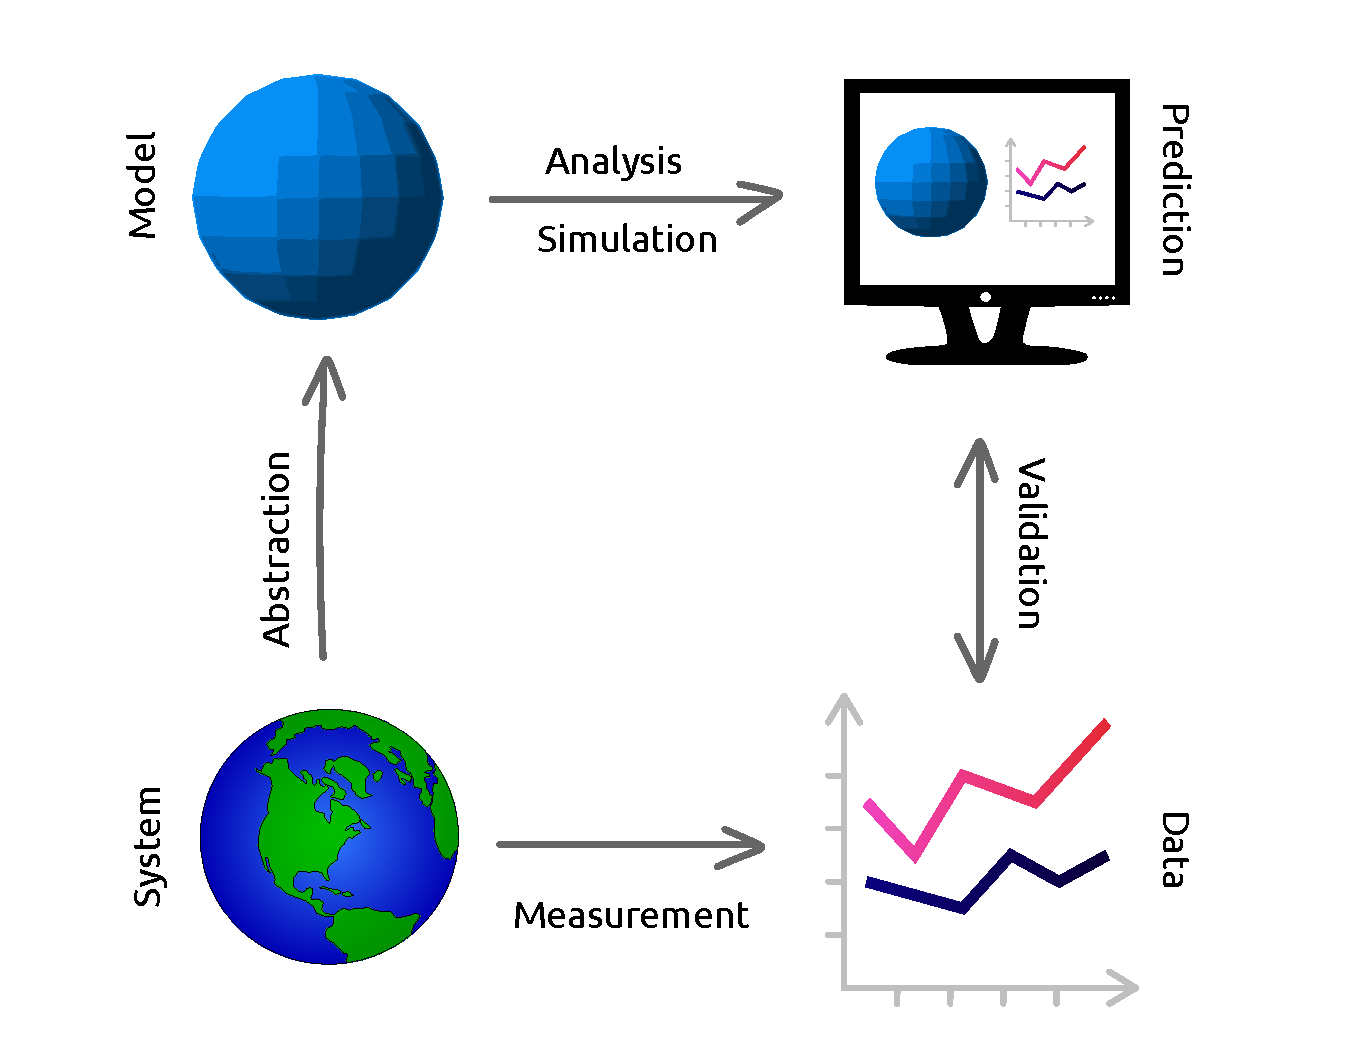
\includegraphics[height=3in]{figs/modeling_framework.pdf}}

Starting in the lower left, the {\bf system} is something in the real world we are interested in.  Often, it is something complicated, so we have to decide which details can be left out; removing details is called {\bf abstraction}.

\index{system}

The result of abstraction is a {\bf model}, which is a description of the system that includes only the features we think are essential.  A model can be represented in the form of diagrams and equations, which can be used for mathematical {\bf analysis}.  It can also be implemented in the form of a computer program, which can run {\bf simulations}.

\index{model}
\index{abstraction}
\index{analysis}

The result of analysis and simulation might be a {\bf prediction} about what the system will do, an {\bf explanation} of why it behaves the way it does, or a {\bf design} intended to achieve a purpose.

\index{prediction}
\index{explanation}
\index{design}

We can {\bf validate} predictions and test designs by taking {\bf measurements} from the real world and comparing the {\bf data} we get with the results from analysis and simulation. 

\index{validation}
\index{data}

For any physical system, there are many possible models, each one including and excluding different features, or including different levels of detail.  The goal of the modeling process is to find the model best suited to its purpose (prediction, explanation, or design).

\index{iterative modeling}

Sometimes the best model is the most detailed.  If we include more features, the model is more realistic, and we expect its predictions to be more accurate.

\index{realism}

But often a simpler model is better.  If we include only the essential features and leave out the rest, we get models that are easier to work with, and the explanations they provide can be clearer and more compelling.

\index{simplicity}

As an example, suppose someone asks you why the orbit of the Earth is elliptical.  If you model the Earth and Sun as point masses (ignoring their actual size), compute the gravitational force between them using Newton's law of universal gravitation, and compute the resulting orbit using Newton's laws of motion, you can show that the result is an ellipse.

\index{orbit}
\index{ellipse}

Of course, the actual orbit of Earth is not a perfect ellipse, because of the gravitational forces of the Moon, Jupiter, and other objects in the solar system, and because Newton's laws of motion are only approximately true (they don't take into account relativistic effects).

\index{Newton}
\index{relativity}

But adding these features to the model would not improve the explanation; more detail would only be a distraction from the fundamental cause.  However, if the goal is to predict the position of the Earth with great precision, including more details might be necessary.  

Choosing the best model depends on what the model is for.  It is usually a good idea to start with a simple model, even if it is likely to be too simple, and test whether it is good enough for its purpose.  Then you can add features gradually, starting with the ones you expect to be most essential.  This process is called {\bf iterative modeling}.

Comparing results of successive models provides a form of {\bf internal validation}, so you can catch conceptual, mathematical, and software errors.  And by adding and removing features, you can tell which ones have the biggest effect on the results, and which can be ignored.

\index{internal validation}
\index{validation!internal}
\index{external validation}
\index{validation!external}

Comparing results to data from the real world provides {\bf external validation}, which is generally the strongest test.


\section{The falling penny myth}
\label{penny}

Let's see an example of how models are used.  You might have heard that a penny dropped from the top of the Empire State Building would be going so fast when it hit the pavement that it would be embedded in the concrete; or if it hit a person, it would break their skull.

\index{Empire State Building}
\index{penny}
\index{myth}

We can test this myth by making and analyzing a model.  To get started, we'll assume that the effect of air resistance is small.  This will turn out to be a bad assumption, but bear with me.

If air resistance is negligible, the primary force acting on the penny is gravity, which causes the penny to accelerate downward.
\index{air resistance}

If the initial velocity is 0, the velocity after $t$ seconds is $a t$, and the distance the penny has dropped is
%
\[ h = a t^2 / 2 \]
%
Using algebra, we can solve for $t$:
%
\[ t = \sqrt{ 2 h / a} \]
%
Plugging in the acceleration of gravity, $a = \SI{9.8}{\meter\per\second\squared}$, and the height of the Empire State Building, $h=\SI{381}{\meter}$, we get $t = \SI{8.8}{\second}$.  Then computing $v = a t$ we get a velocity on impact of $\SI{86}{\meter\per\second}$, which is about 190 miles per hour.  That sounds like it could hurt.

Of course, these results are not exact because the model is based on simplifications.  For example, we assume that gravity is constant.  In fact, the force of gravity is different on different parts of the globe, and gets weaker as you move away from the surface.  But these differences are small, so ignoring them is probably a good choice for this scenario.
\index{gravity}

On the other hand, ignoring air resistance is not a good choice.  Once the penny gets to about \SI{18}{\meter\per\second}, the upward force of air resistance equals the downward force of gravity, so the penny stops accelerating.  After that, it doesn't matter how far the penny falls; it hits the sidewalk (or your head) at about \SI{18}{\meter\per\second}, much less than \SI{86}{\meter\per\second}, as the simple model predicts.

The statistician George Box famously said ``All models are wrong, but some are useful."  He was talking about statistical models, but his wise words apply to all kinds of models.  Our first model, which ignores air resistance, is very wrong, and probably not useful.  In the notebook for this chapter, you will see another model, which assumes that acceleration is constant until the penny reaches terminal velocity.  This model is also wrong, but it's better, and it's good enough to refute the myth.

\index{Box, George}

The television show {\it Mythbusters} has tested the myth of the falling penny more carefully; you can view the results at \url{http://modsimpy.com/myth}.  Their work is based on a mathematical model of motion, measurements to determine the force of air resistance on a penny, and a physical model of a human head.

\index{Mythbusters}


\section{Computation}
\label{computation}

There are (at least) two ways to work with mathematical models, {\bf analysis} and {\bf simulation}.  Analysis often involves algebra and other kinds of symbolic manipulation.  Simulation often involves computers.
\index{analysis}
\index{simulation}

In this book we do some analysis and a lot of simulation; along the way, I discuss the pros and cons of each.  The primary tools we use for simulation are the Python programming language and Jupyter, which is an environment for writing and running programs.

As a first example, I'll show you how I computed the results from the previous section using Python.

First I create a {\bf variable} to represent acceleration.

\index{variable}
\index{value}

\begin{python}
a = 9.8 * meter / second**2
\end{python}

A variable is a name that corresponds to a value.  In this example, the name is \py{a} and the value is the number \py{9.8} multiplied by the units \py{meter / second**2}.  This example demonstrates some of the symbols Python uses to perform mathematical operations:
\index{operator!mathematical}

\begin{tabular}{l|c}
{\bf Operation} & {\bf Symbol} \\ 
\hline 
Addition & \py{+} \\ 
Subtraction & \py{-} \\ 
Multiplication & \py{*} \\ 
Division & \py{/} \\ 
Exponentiation & \py{**}  \\ 
\end{tabular} 

Next, we compute the time it takes for the penny to drop \SI{381}{\meter}, the height of the Empire State Building.

\begin{python}
h = 381 * meter
t = sqrt(2 * h / a)
\end{python}

These lines create two more variables: \py{h} gets the height of the building in meters; \py{t} gets the time, in seconds, for the penny to fall to the sidewalk.  \py{sqrt} is a {\bf function} that computes square roots.  Python keeps track of units, so the result, \py{t}, has the correct units, seconds.
\index{unit}
\index{function}
\index{sqrt}

Finally, we compute the velocity of the penny after $t$ seconds:

\begin{python}
v = a * t
\end{python}

The result is about \SI{86}{\meter\per\second}, again with the correct units.

This example demonstrates analysis and computation using Python.  In the next chapter, we'll see an example of simulation.  

Before you go on, you might want to read the notebook for this chapter, \py{chap01.ipynb}, and work on the exercises.  For instructions on downloading and running the code, see Section~\ref{code}.


\chapter{Bike share}
\label{chap02}

This chapter presents a simple model of a bike share system and demonstrates the features of Python we'll use to develop simulations of real-world systems.  

Along the way, we'll make decisions about how to model the system.  In the next chapter we'll review these decisions and gradually improve the model.


\section{Modeling}
\label{modeling}

Imagine a bike share system for students traveling between Olin College and Wellesley College, which are about 3 miles apart in eastern Massachusetts.

\index{Wellesley College}
\index{Olin College}

Suppose the system contains 12 bikes and two bike racks, one at Olin and one at Wellesley, each with the capacity to hold 12 bikes.

\index{bike share system}

As students arrive, check out a bike, and ride to the other campus, the number of bikes in each location changes.  In the simulation, we'll need to keep track of where the bikes are.  To do that, I'll create a \py{State} object, which is defined in the ModSim library.  

\index{State object}

Before we can use the library, we have to \py{import} it:

\begin{python}
from modsim import *
\end{python}

This line of code is an {\bf import statement} that tells Python
to read the file {\tt modsim.py} and make the functions it defines available.

\index{import statement}

Functions in the \py{modsim.py} library include \py{sqrt}, which we used in the previous section, and \py{State}, which we are using now.  \py{State} creates a \py{State} object, which is a collection of {\bf state variables}.  

\index{state variable}

\begin{python}
bikeshare = State(olin=10, wellesley=2)
\end{python}

The state variables, \py{olin} and \py{wellesley}, represent the number of bikes at each location.  The initial values are 10 and 2, indicating that there are 10 bikes at Olin and 2 at Wellesley.  The \py{State} object created by \py{State} is assigned to a new variable named \py{bikeshare}.

\index{dot operator}
\index{operator!dot}

We can read the variables inside a \py{State} object using the {\bf dot operator}, like this:

\begin{python}
bikeshare.olin
\end{python}

The result is the value 10.  Similarly, for:

\begin{python}
bikeshare.wellesley
\end{python}

The result is 2.  If you forget what variables a state object has, you can just type the name:

\begin{python}
bikeshare
\end{python}

The result looks like a table with the variable names and their values:

\begin{tabular}{lr}
 & {\bf \sf value} \\ 
\hline 
{\bf \sf olin} & 10 \\ 
{\bf \sf wellesley} & 2 \\ 
\end{tabular} 

The state variables and their values make up the {\bf state} of the system.  We can update the state by assigning new values to the variables.  For example, if a student moves a bike from Olin to Wellesley, we can figure out the new values and assign them:

\index{state}

\begin{python}
bikeshare.olin = 9
bikeshare.wellesley = 3
\end{python}

Or we can use {\bf update operators}, \py{-=} and \py{+=}, to subtract 1 from \py{olin} and add 1 to \py{wellesley}:

\index{update operator}
\index{operator!update}

\begin{python}
bikeshare.olin -= 1
bikeshare.wellesley += 1
\end{python}

The result is the same either way, but the second version is more versatile.


\section{Defining functions}

So far we have used functions defined in ModSim and other libraries.  Now we're going to define our own functions.

\index{function}
\index{defining functions}

When you are developing code in Jupyter, it is often efficient to
write a few lines of code, test them to confirm they do what
you intend, and then use them to define a new function.  For
example, these lines move a bike from Olin to Wellesley:

\begin{python}
bikeshare.olin -= 1
bikeshare.wellesley += 1
\end{python}

Rather than repeat them every time a bike moves, we can define a
new function:

\begin{python}
def bike_to_wellesley():
    bikeshare.olin -= 1
    bikeshare.wellesley += 1
\end{python}

\py{def} is a special word in Python that indicates we are defining a new
function.  The name of the function is \py{bike_to_wellesley}.  The empty parentheses indicate that this function requires no additional information when it runs.  The colon indicates the beginning of an indented
{\bf code block}.
\index{def}
\index{code block}
\index{body}
\index{indentation}

The next two lines are the {\bf body} of the function.  They have to be indented; by convention, the indentation is 4 spaces.

When you define a function, it has no immediate effect.  The body
of the function doesn't run until you {\bf call} the function.
Here's how to call this function:
\index{call}

\begin{python}
bike_to_wellesley()
\end{python}

When you call the function, it runs the statements in the body, which update the variables of the {\tt bikeshare} object; you can check by displaying the new state.

When you call a function, you have to include the parentheses.  If you leave them out, like this:
\index{parentheses}

\begin{python}
bike_to_wellesley
\end{python}

Python looks up the name of the function and displays:

\begin{python}
<function __main__.bike_to_wellesley>
\end{python}

This result indicates that \py{bike_to_wellesley} is a function.  You don't have to know what \py{__main__} means, but if you see something like this, it probably means that you looked up a function but you didn't
actually call it.  So don't forget the parentheses.

Just like \py{bike_to_wellesley}, we can define a function that moves a bike from Wellesley to Olin:

\begin{python}
def bike_to_olin():
    bikeshare.wellesley -= 1
    bikeshare.olin += 1
\end{python}

And call it like this:

\begin{python}
bike_to_olin()
\end{python}

One benefit of defining functions is that you avoid repeating chunks
of code, which makes programs smaller.  Another benefit is that the
name you give the function documents what it does, which makes programs
more readable.


\section{Print statements}

As you write more complicated programs, it is easy to lose track of what is going on.  One of the most useful tools for debugging is the {\bf print statement}, which displays text in the Jupyter notebook.
\index{print statement}
\index{statement!print}

Normally when Jupyter runs the code in a cell, it displays the value of the last line of code.  For example, if you run:

\begin{python}
bikeshare.olin
bikeshare.wellesley
\end{python}

Jupyter runs both lines of code, but it only displays the value of the second line.  If you want to display more than one value, you can use print statements:

\begin{python}
print(bikeshare.olin)
print(bikeshare.wellesley)
\end{python}

When you call the \py{print} function, you can put a variable name in parentheses, as in the previous example, or you can provide a sequence of variables separated by commas, like this:

\begin{python}
print(bikeshare.olin, bikeshare.wellesley)
\end{python}

Python looks up the values of the variables and displays them; in this example, it displays two values on the same line, with a space between them.

Print statements are useful for debugging functions.  For example, we can add a print statement to \py{move_bike}, like this:

\begin{python}
def bike_to_wellesley():
    print('Moving a bike to Wellesley')
    bikeshare.olin -= 1
    bikeshare.wellesley += 1
\end{python}

Each time we call this version of the function, it displays a message, which can help us keep track of what the program is doing.

The message in this example is a {\bf string}, which is a sequence of letters and other symbols in quotes.
\index{string}


\section{If statements}

The ModSim library provides a function called \py{flip}; when you call it, you provide a value between 0 and 1; in this example, it's \py{0.7}:

\begin{python}
flip(0.7)
\end{python}

The result is one of two values: \py{True} with probability 0.7 or \py{False} with probability 0.3.  If you run \py{flip} like this 100 times, you should get \py{True} about 70 times and \py{False} about 30 times.  But the results are random, so they might differ from these expectations.
\index{flip}
\index{True}
\index{False}

\py{True} and \py{False} are special values defined by Python.  Note
that they are not strings.  There is a difference between \py{True},
which is a special value, and \py{'True'}, which is a string.
\index{string}
\index{boolean}

\py{True} and \py{False} are called {\bf boolean} values because
they are related to Boolean algebra (\url{http://modsimpy.com/boolean}).

We can use boolean values to control the behavior of the program, using
an {\bf if statement}:
\index{if statement}
\index{statement!if}

\begin{python}
if flip(0.5):
    print('heads')
\end{python}

If the result from \py{flip} is \py{True}, the program displays the string \py{'heads'}.  Otherwise it does nothing.

The punctuation for \py{if} statements is similar to the punctuation for function definitions: the first line has to end with a colon, and the lines inside the \py{if} statement have to be indented.
\index{indentation}
\index{else clause}

Optionally, you can add an {\bf else clause} to indicate what should happen if the result is \py{False}:

\begin{python}
if flip(0.5):
    print('heads')
else:
    print('tails')    
\end{python}

Now we can use \py{flip} to simulate the arrival of students who want to borrow a bike.  Suppose students arrive at the Olin station every 2 minutes, on average.  In that case, the chance of an arrival during any one-minute period is 50\%, and we can simulate it like this:

\begin{python}
if flip(0.5):
    bike_to_wellesley()
\end{python}

If students arrive at the Wellesley station every 3 minutes, on average, the chance of an arrival during any one-minute period is 33\%, and we can simulate it like this:

\begin{python}
if flip(0.33):
    bike_to_olin()
\end{python}

We can combine these snippets into a function that simulates a {\bf time step}, which is an interval of time, in this case one minute:

\index{time step}

\begin{python}
def step():
    if flip(0.5):
        bike_to_wellesley()
    
    if flip(0.33):
        bike_to_olin()
\end{python}

Then we can simulate a time step like this:

\begin{python}
step()
\end{python}

Even though there are no values in parentheses, we have to include them.


\section{Parameters}

The previous version of \py{step} is fine if the arrival probabilities never change, but in reality, these probabilities vary over time.

So instead of putting the constant values 0.5 and 0.33 in \py{step} we can replace them with {\bf parameters}.  Parameters are variables whose values are set when a function is called.

Here's a version of \py{step} that takes two parameters, \py{p1} and \py{p2}:

\index{probability}

\begin{python}
def step(p1, p2):
    if flip(p1):
        bike_to_wellesley()
    
    if flip(p2):
        bike_to_olin()
\end{python}

The values of \py{p1} and \py{p2} are not set inside this function; instead, they are provided when the function is called, like this:

\begin{python}
step(0.5, 0.33)
\end{python}

The values you provide when you call the function are called {\bf arguments}.
The arguments, \py{0.5} and \py{0.33} in this example, get assigned to the parameters, \py{p1} and \py{p2}, in order.  So running this function has the same effect as:

\begin{python}
p1 = 0.5
p2 = 0.33

if flip(p1):
    bike_to_wellesley()
    
if flip(p2):
    bike_to_olin()
\end{python}

The advantage of using parameters is that you can call the same function many times, providing different arguments each time.  

Adding parameters to a function is called {\bf generalization}, because it makes the function more general, that is, less specialized.

\index{generalization}


\section{For loops}
\label{forloop}

At some point you will get sick of running cells over and over. Fortunately, there is an easy way to repeat a chunk of code, the {\bf for loop}.  Here's an example:
\index{for loop}
\index{loop}

\begin{python}
for i in range(4):
    bike_to_wellesley()
\end{python}

The punctuation here should look familiar; the first line ends with a colon, and the lines inside the \py{for} loop are indented.  The other elements of the loop are:
\index{range}

\begin{itemize}

\item The words \py{for} and \py{in} are special words we have to use in a for loop.  

\item \py{range} is a Python function we're using here to control the number of times the loop runs.
\index{range}

\item \py{i} is a {\bf loop variable} that gets created when the for loop runs. 
\index{loop variable}

\end{itemize}

In this example we don't actually use \py{i}; we will see examples later where we use the loop variable inside the loop.

When this loop runs, it runs the statements inside the loop four times, 
which moves one bike at a time from Olin to Wellesley.


\section{TimeSeries}
\label{timeseries}

When we run a simulation, we usually want to save the results for later analysis.  The ModSim library provides a \py{TimeSeries} object for this purpose.  A \py{TimeSeries} contains a sequence of time stamps and a corresponding sequence of values.  In this example, the time stamps are integers representing minutes, and the values are the number of bikes at one location.

%TODO: index modsim library functions
\index{ModSim library}
\index{TimeSeries}

We can create a new, empty \py{TimeSeries} like this:

\begin{python}
results = TimeSeries()
\end{python}

And we can add a value to a \py{TimeSeries} like this:

\begin{python}
results[0] = bikeshare.olin
\end{python}

The number in brackets is the time stamp, also called a {\bf label}.
\index{label}

We can use a \py{TimeSeries} inside a for loop to store the results of the simulation:

\begin{python}
for i in range(10):
    step(0.3, 0.2)
    results[i] = bikeshare.olin
\end{python}

Each time through the loop, we call \py{step}, which updates \py{bikeshare}.  Then we store the number of bikes at Olin in \py{results}.  We use the loop variable, \py{i}, as the time stamp.

\index{loop}
\index{loop variable}
\index{time stamp}

When the loop exits, \py{results} contains 10 time stamps, from 0 through 9, and the number of bikes at Olin at the end of each time step.
\index{loop variable}

\py{TimeSeries} is a specialized version of \py{Series}, which is defined by Pandas, one of the libraries we'll be using extensively.  The \py{Series} object provides many functions; one example is \py{mean}, which we can call like this:

\begin{python}
results.mean()
\end{python}

You can read the documentation of \py{Series} at \url{http://modsimpy.com/series}.

\index{Pandas}
\index{Series}
\index{TimeSeries}
\index{mean}


\section{Plotting}
\label{plotting}

The ModSim library provides a function called \py{plot} we can use to plot \py{results}:

\begin{python}
plot(results)
\end{python}

\py{plot} can take an additional argument that gives the line a label; this label will appear in the legend of the plot, if we create one.

\begin{python}
plot(results, label='Olin')
\end{python}

\py{label} is an example of a {\bf keyword argument}, so called because we provide a ``keyword'', which is \py{label} in this case, along with its value.  Arguments without keywords are called {\bf positional arguments} because they are assigned to parameters according to their position.  It is good to know these terms because they appear in Python error messages.

\index{keyword argument}
\index{positional argument}
\index{argument}

Whenever you make a figure, you should label the axes.  The ModSim library provides \py{decorate}, which labels the axes and gives the figure a title and legend:

\begin{python}
decorate(title='Olin-Wellesley Bikeshare',
         xlabel='Time step (min)', 
         ylabel='Number of bikes')
\end{python}

\begin{figure}
\centerline{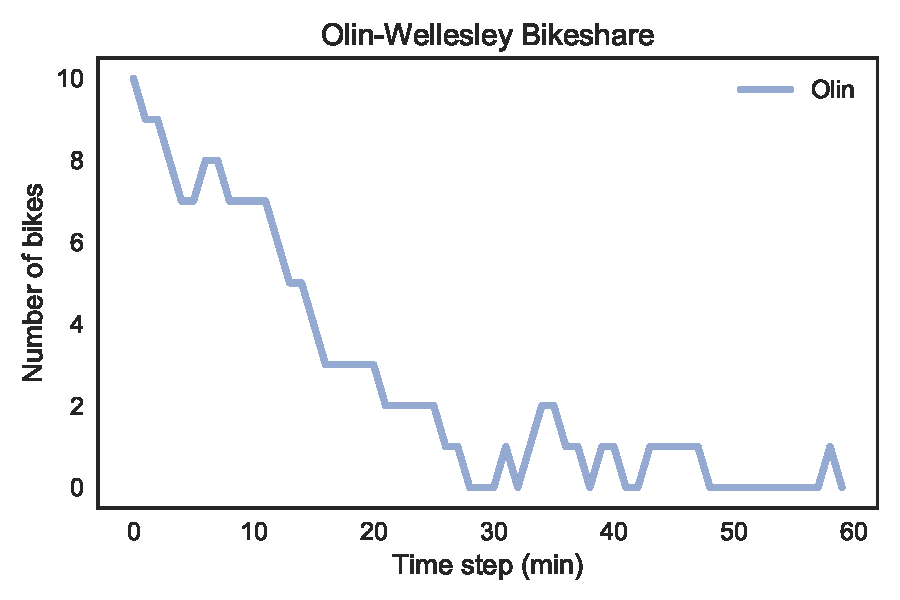
\includegraphics[height=3in]{figs/chap02-fig01.pdf}}
\caption{Simulation of a bikeshare system showing number of bikes at Olin over time.}
\label{chap02-fig01}
\end{figure}

Figure~\ref{chap02-fig01} shows the result.

\py{plot} and \py{decorate} are based on Pyplot, which is a Python library for generating figures.  You can read more about \py{plot} and the arguments it takes at \url{http://modsimpy.com/plot}.

\index{Pyplot}
\index{plot}
\index{decorate}

Before you go on, you might want to read the notebook for this chapter, \py{chap02.ipynb}, and work on the exercises.  For instructions on downloading and running the code, see Section~\ref{code}.



\chapter{Iterative modeling}
\label{chap03}

To paraphrase two Georges, ``All models are wrong, but some models are more wrong than others."  In this chapter, I demonstrate the process we use to make models less wrong.

\index{Box, George}
\index{Orwell, George}

As an example, we'll review the bikeshare model from the previous chapter, consider its strengths and weaknesses, and gradually improve it.  We'll also see ways to use the model to understand the behavior of the system and evaluate designs intended to make it work better.

\index{bikeshare}


\section{Iterative modeling}

The model we have so far is simple, but it is based on unrealistic assumptions.  Before you go on, take a minute to review the model from the previous chapters.  What assumptions is it based on?  Make a list of ways this model might be unrealistic; that is, what are the differences between the model and the real world?

Here are some of the differences on my list:

\begin{itemize}

\item In the model, a student is equally likely to arrive during any one-minute period.  In reality, this probability varies depending on time of day, day of the week, etc.

\index{probability}

\item The model does not account for travel time from one bike station to another.

\item The model does not check whether a bike is available, so it's possible for the number of bikes to be negative (as you might have noticed in some of your simulations).

\end{itemize}

Some of these modeling decisions are better than others.  For example, the first assumption might be reasonable if we simulate the system for a short period of time, like one hour.

The second assumption is not very realistic, but it might not affect the results very much, depending on what we use the model for.

\index{realism}

On the other hand, the third assumption seems problematic, and it is relatively easy to fix.  In Section~\ref{negativebikes}, we will.

This process, starting with a simple model, identifying the most important problems, and making gradual improvements, is called {\bf iterative modeling}.

\index{iterative modeling}

For any physical system, there are many possible models, based on different assumptions and simplifications.  It often takes several iterations to develop a model that is good enough for the intended purpose, but no more complicated than necessary.


\section{More than one State object}

Before we go on, I want to make a few changes to the code from the previous chapter.  First I'll generalize the functions we wrote so they take a \py{State} object as a parameter.  Then, I'll make the code more readable by adding documentation.

\index{parameter}

Here is one of the functions from the previous chapter, \py{bike_to_wellesley}:

\begin{python}
def bike_to_wellesley():
    bikeshare.olin -= 1
    bikeshare.wellesley += 1
\end{python}

When this function is called, it modifies \py{bikeshare}.  As long as there is only one \py{State} object, that's fine, but what if there is more than one bike share system in the world?  Or what if we want to run more than one simulation?

This function would be more flexible if it took a \py{State} object as a parameter.  Here's what that looks like:

\index{State object}

\begin{python}
def bike_to_wellesley(state):
    state.olin -= 1
    state.wellesley += 1
\end{python}

The name of the parameter is \py{state} rather than \py{bikeshare} as a reminder that the value of \py{state} could be any \py{State} object, not just \py{bikeshare}.

This version of \py{bike_to_wellesley} requires a \py{State} object as a parameter, so we have to provide one when we call it:

\begin{python}
bike_to_wellesley(bikeshare)
\end{python}

Again, the argument we provide gets assigned to the parameter, so this function call has the same effect as:

\begin{code}
state = bikeshare
state.olin -= 1
state.wellesley += 1
\end{code}

Now we can create as many \py{State} objects as we want:

\begin{python}
bikeshare1 = State(olin=10, wellesley=2)
bikeshare2 = State(olin=2, wellesley=10)
\end{python}

And update them independently:

\begin{python}
bike_to_wellesley(bikeshare1)
bike_to_wellesley(bikeshare2)
\end{python}

Changes in \py{bikeshare1} do not affect \py{bikeshare2}, and vice versa.  So we can simulate different bike share systems, or run multiple simulations of the same system.


\section{Documentation}
\label{documentation}

Another problem with the code we have so far is that it contains no {\bf documentation}.  Documentation is text we add to a program to help other programmers read and understand it.  It has no effect on the program when it runs.

\index{documentation}
\index{docstring}
\index{comment}

There are two forms of documentation, {\bf docstrings} and {\bf comments}.   
 A docstring is a string in triple-quotes that appears at the beginning of a function, like this:

\begin{python}
def run_simulation(state, p1, p2, num_steps):
    """Simulate the given number of time steps.
    
    state: State object
    p1: probability of an Olin->Wellesley customer arrival
    p2: probability of a Wellesley->Olin customer arrival
    num_steps: number of time steps
    """
    results = TimeSeries()    
    for i in range(num_steps):
        step(state, p1, p2)
        results[i] = state.olin
        
    plot(results, label='Olin')
\end{python}

Docstrings follow a conventional format:

\begin{itemize}

\item The first line is a single sentence that describes what the function does.

\item The following lines explain what each of the parameters are.

\end{itemize}

A function's docstring should include the information someone needs to know to {\em use} the function; it should not include details about how the function works.  That's what comments are for.

A comment is a line of text that begins with a hash symbol, \py{#}.  It usually appears inside a function to explain something that would not be obvious to someone reading the program.

\index{comment}
\index{hash symbol}

For example, here is a version of \py{bike_to_olin} with a docstring and a comment.

\begin{python}
def bike_to_olin(state):
	"""Move one bike from Wellesley to Olin.
	
	state: State object	
	"""
	# We decrease one state variable and increase the
	# other, so the total number of bikes is unchanged.
    state.wellesley -= 1
    state.olin += 1
\end{python}

At this point we have more documentation than code, which is not unusual for short functions.


\section{Negative bikes}
\label{negativebikes}

The changes we've made so far improve the quality of the code, but we haven't done anything to improve the quality of the model yet.   Let's do that now.

\index{code quality}

Currently the simulation does not check whether a bike is available when a customer arrives, so the number of bikes at a location can be negative.  That's not very realistic.  Here's an updated version of \py{bike_to_olin} that fixes the problem:

\begin{python}
def bike_to_olin(state):
    if state.wellesley == 0:
        return
    state.wellesley -= 1
    state.olin += 1
\end{python}

The first line checks whether the number of bikes at Wellesley is zero.  If so, it uses a {\bf return statement}, which causes the function to end immediately, without running the rest of the statements.  So if there are no bikes at Wellesley, we ``return" from \py{bike_to_olin} without changing the state.

\index{return statement}
\index{statement!return}

We can update \py{bike_to_wellesley} the same way.


\section{Comparison operators}

The version of \py{bike_to_olin} in the previous section uses the equals operator, \py{==}, which compares two values and returns \py{True} if they are equal and \py{False} otherwise.

It is easy to confuse the equals operators with the assignment operator, \py{=}, which assigns a value to a variable.  For example, the following statement creates a variable, \py{x}, if it doesn't already exist, and gives it the value \py{5}.

\index{equality}
\index{assignment operator}
\index{operator!assignment}

\begin{python}
x = 5
\end{python}

On the other hand, the following statement checks whether \py{x} is \py{5} and returns \py{True} or \py{False}.  It does not create \py{x} or change its value.  

\begin{python}
x == 5
\end{python}

You can use the equals operator in an \py{if} statement, like this:

\index{if statement}
\index{statement!if}

\begin{python}
if x == 5:
    print('yes, x is 5')
\end{python}

If you make a mistake and use \py{=} in an \py{if} statement, like this:

\begin{python}
if x = 5:
    print('yes, x is 5')
\end{python}

That's a {\bf syntax error}, which means that the structure of the program is invalid.  Python will print an error message and the program won't run.

\index{syntax error}
\index{error!syntax}

The equals operator is one of the {\bf comparison operators}. The others are:

\index{comparison operator}
\index{operator!comparison}

\begin{tabular}{l|c}
{\bf Operation} & {\bf Symbol} \\ 
\hline 
Less than & \py{<} \\ 
Greater than & \py{>} \\
Less than or equal & \py{<=}  \\ 
Greater than or equal & \py{>=} \\ 
Equal & \py{==} \\ 
Not equal & \py{!=} \\ 
\end{tabular} 


\section{Metrics}
\label{metrics}

Getting back to the bike share system, at this point we have the ability to simulate the behavior of the system.  Since the arrival of customers is random, the state of the system is different each time we run a simulation.  Models like this are called random or {\bf stochastic}; models that do the same thing every time they run are {\bf deterministic}.

\index{stochastic}
\index{deterministic}

Suppose we want to use our model to predict how well the bike share system will work, or to design a system that works better.  First, we have to decide what we mean by ``how well" and ``better".

From the customer's point of view, we might like to know the probability of finding an available bike.  From the system-owner's point of view, we might want to minimize the number of customers who don't get a bike when they want one, or maximize the number of bikes in use.  Statistics like these that quantify how well the system works are called {\bf metrics}.

\index{metric}

As a simple example, let's measure the number of unhappy customers.  Here's a version of \py{bike_to_olin} that keeps track of the number of customers who arrive at a station with no bikes:

\begin{python}
def bike_to_olin(state):
    if state.wellesley == 0:
        state.wellesley_empty += 1
        return
    state.wellesley -= 1
    state.olin += 1
\end{python}

If a customer arrives at the Wellesley station and finds no bike available, \py{bike_to_olin} updates \py{wellesley_empty} which counts the number of unhappy customers.

This function only works if we initialize \py{wellesley_empty} when we create the \py{State} object, like this:

\begin{python}
bikeshare = State(olin=10, wellesley=2, 
                  olin_empty=0, wellesley_empty=0)
\end{python}

Assuming we update \py{move_to_wellesley} the same way, we can run the simulation like this (see Section~\ref{documentation}):

\begin{python}
run_simulation(bikeshare, 0.4, 0.2, 60)
\end{python}

Then we can check the metrics:

\begin{python}
print(bikeshare.olin_empty, bikeshare.wellesley_empty)
\end{python}

Because the simulation is stochastic, the results are different each time it runs.

Before you go on, you might want to read the notebook for this chapter, \py{chap03.ipynb}, and work on the exercises.  For instructions on downloading and running the code, see Section~\ref{code}.


\chapter{Sweeping parameters}
\label{chap04}

In the previous chapter we defined metrics that quantify the performance of bike sharing this system.  In this chapter we see how those metrics depend on the parameters of the system, like the arrival rate of customers at bike stations.

We also discuss a program development strategy, called incremental development, that might help you write programs faster and spend less time debugging.


\section{Functions that return values}

We have seen several functions that return values; for example, when you run \py{sqrt}, it returns a number you can assign to a variable.

\index{return value}

\begin{python}
t = sqrt(2 * h / a)
\end{python}

When you run \py{State}, it returns a new \py{State} object:
 
\begin{python}
bikeshare = State(olin=10, wellesley=2)
\end{python}

Not all functions have return values.  For example, when you run \py{step}, it updates a \py{State} object, but it doesn't return a value.

To write functions that return values, we can use a second form of the \py{return} statement, like this:

\index{return statement}
\index{statement!return}

\begin{python}
def add_five(x):
    return x + 5
\end{python}

\py{add_five} takes a parameter, \py{x}, which could be any number.  It computes \py{x + 5} and returns the result.  So if we run it like this, the result is \py{8}:

\begin{python}
add_five(3)
\end{python}

As a more useful example, here's a version of \py{run_simulation} that creates a \py{State} object, runs a simulation, and then returns the \py{State} object as a result:

\begin{python}
def run_simulation():
    p1 = 0.4
    p2 = 0.2
    num_steps = 60
    
    state = State(olin=10, wellesley=2, 
                    olin_empty=0, wellesley_empty=0)
                    
    for i in range(num_steps):
        step(state, p1, p2)
        
    return state
\end{python}

If we call \py{run_simulation} like this:

\begin{python}
state = run_simulation()
\end{python}

It assigns the \py{State} object from \py{run_simulation} to \py{state}, which contains the metrics we are interested in:

\begin{python}
print(state.olin_empty, state.wellesley_empty)
\end{python}


\section{Two kinds of parameters}

This version of \py{run_simulation} always starts with the same initial condition, 10 bikes at Olin and 2 bikes at Wellesley, and the same values of \py{p1}, \py{p2}, and \py{num_steps}.  Taken together, these five values are the {\bf parameters of the model}, which are values that determine the behavior of the system.

\index{parameter!of a model}
\index{parameter!of a function}

It is easy to get the parameters of a model confused with the parameters of a function.  They are closely related ideas; in fact, it is common for the parameters of the model to appear as parameters in functions.  For example, we can write a more general version of \py{run_simulation} that takes \py{p1} and \py{p2} as function parameters:

\begin{python}
def run_simulation(p1, p2, num_steps):
    state = State(olin=10, wellesley=2, 
                    olin_empty=0, wellesley_empty=0)
                    
    for i in range(num_steps):
        step(state, p1, p2)
        
    return state
\end{python}

Now we can run it with different arrival rates, like this:

\begin{python}
state = run_simulation(0.6, 0.3, 60)
\end{python}

In this example, \py{0.6} gets assigned to \py{p1}, \py{0.3} gets assigned to \py{p2}, and \py{60} gets assigned to \py{num_steps}.

Now we can call \py{run_simulation} with different parameters and see how the metrics, like the number of unhappy customers, depend on the parameters.  But before we do that, we need a new version of a for loop.

\index{metric}


\section{Loops and arrays}
\label{array}

In Section~\ref{forloop}, we saw a loop like this:

\begin{python}
for i in range(4):
    bike_to_wellesley()
\end{python}

\py{range(4)} creates a sequence of numbers from 0 to 3.  Each time through the loop, the next number in the sequence gets assigned to the loop variable, \py{i}.

\index{loop}
\index{loop variable}
\index{variable!loop}

\py{range} only works with integers; to get a sequence of non-integer values, we can use \py{linspace}, which is defined in the ModSim library:

\begin{python}
p1_array = linspace(0, 1, 5)
\end{python}

The arguments indicate where the sequence should start and stop, and how many elements it should contain.  In this example, the sequence contains \py{5} equally-spaced numbers, starting at \py{0} and ending at \py{1}. 

\index{linspace}
\index{NumPy}
\index{array}

The result is a NumPy {\bf array}, which is a new kind of object we have not seen before.  An array is a container for a sequence of numbers.

We can use an array in a \py{for} loop like this:

\begin{python}
for p1 in p1_array:
    print(p1)
\end{python}

When this loop runs, it

\begin{enumerate}

\item Gets the first value from the array and assigns it to \py{p1}.

\item Runs the body of the loop, which prints \py{p1}.

\item Gets the next value from the array and assigns it to \py{p1}.

\item Runs the body of the loop, which prints \py{p1}.

\end{enumerate}

And so on, until it gets to the end of the array.  The result is:

\begin{result}
0.0
0.25
0.5
0.75
1.0
\end{result}

This will come in handy in the next section.


\section{Sweeping parameters}

If we know the actual values of parameters like \py{p1} and \py{p2}, we can use them to make specific predictions, like how many bikes will be at Olin after one hour.

\index{prediction}
\index{explanation}

But prediction is not the only goal; models like this are also used to explain why systems behave as they do and to evaluate alternative designs.  For example, if we observe the system and notice that we often run out of bikes at a particular time, we could use the model to figure out why that happens.  And if we are considering adding more bikes, or another station, we could evaluate the effect of various ``what if" scenarios.
\index{what if scenario}

As an example, suppose we have enough data to estimate that \py{p2} is about \py{0.2}, but we don't have any information about \py{p1}.  We could run simulations with a range of values for \py{p1} and see how the results vary.  This process is called {\bf sweeping} a parameter, in the sense that the value of the parameter ``sweeps" through a range of possible values.

\index{sweep}
\index{parameter sweep}

Now that we know about loops and arrays, we can use them like this:

\begin{python}
p1_array = linspace(0, 1, 11)
p2 = 0.2
num_steps = 60

for p1 in p1_array:
    state = run_simulation(p1, p2, num_steps)
    print(p1, state.olin_empty)
\end{python}

Each time through the loop, we run a simulation with a different value of \py{p1} and the same value of \py{p2}, \py{0.2}.  Then we print \py{p1} and the number of unhappy customers at Olin.

To save and plot the results, we can use a \py{SweepSeries} object, which is similar to a \py{TimeSeries}; the difference is that the labels in a \py{SweepSeries} are parameter values rather than time values. 

We can create an empty \py{SweepSeries} like this:

\begin{code}
sweep = SweepSeries()
\end{code}

And add values like this:

\begin{python}
for p1 in p1_array:
    state = run_simulation(p1, p2, num_steps)
    sweep[p1] = state.olin_empty
\end{python}

The result is a \py{SweepSeries} that maps from each value of \py{p1} to the resulting number of unhappy customers.  Then we can plot the results:

\begin{code}
plot(sweep, label='Olin')
\end{code}




\section{Incremental development}

When you start writing programs that are more than a few lines, you
might find yourself spending more and more time debugging.  The more
code you write before you start debugging, the harder it is to find
the problem.

\index{debugging}
\index{incremental development}

{\bf Incremental development} is a way of programming that tries
to minimize the pain of debugging.  The fundamental steps are:

\begin{enumerate}

\item Always start with a working program.  If you have an
example from a book, or a program you wrote that is similar to
what you are working on, start with that.  Otherwise, start with
something you {\em know} is correct, like {\tt x=5}.  Run the program
and confirm that it does what you expect.

\item Make one small, testable change at a time.  A ``testable''
change is one that displays something or has some
other effect you can check.  Ideally, you should know what
the correct answer is, or be able to check it by performing another
computation. 

\index{testable change}

\item Run the program and see if the change worked.  If so, go back
to Step 2.  If not, you will have to do some debugging, but if the
change you made was small, it shouldn't take long to find the problem.

\end{enumerate}

When this process works, your changes usually work the first time, or if they don't, the problem is obvious.  In practice, there are two problems with incremental development:

\begin{itemize}

\item Sometimes you have to write extra code to generate visible output that you can check.  This extra code is called {\bf scaffolding} because you use it to build the program and then remove it when you are done.  That might seem like a waste, but time you spend on scaffolding is almost always time you save on debugging.

\index{scaffolding}

\item When you are getting started, it might not be obvious how to
choose the steps that get from {\tt x=5} to the program you are trying
to write.  You will see more examples of this process as we go along, and you will get better with experience.

\end{itemize}

If you find yourself writing more than a few lines of code before you start testing, and you are spending a lot of time debugging, try incremental development.

Before you go on, you might want to read the notebook for this chapter, \py{chap04.ipynb}, and work on the exercises.  For instructions on downloading and running the code, see Section~\ref{code}.


%\part{Modeling population growth}

\chapter{World population}
\label{chap05}

In 1968 Paul Erlich published {\it The Population Bomb}, in which he predicted that world population would grow quickly during the 1970s, that agricultural production could not keep up, and that mass starvation in the next two decades was inevitable (see \url{http://modsimpy.com/popbomb}).  As someone who grew up during those decades, I am happy to report that those predictions were wrong.
  
\index{Erlich, Paul}
\index{Population Bomb}

But world population growth is still a topic of concern, and it is an open question how many people the earth can sustain while maintaining and improving our quality of life.

\index{world population}
\index{population}

In this chapter and the next, we use tools from the previous chapters to explain world population growth since 1950 and generate predictions for the next 50--100 years.

\index{prediction}

For background on world population growth, watch this video from the American Museum of Natural History \url{http://modsimpy.com/human}.

\index{American Museum of Natural History}


\section{World Population Data}
\label{worldpopdata}

The Wikipedia article on world population contains tables with estimates of world population from prehistory to the present, and projections for the future (\url{http://modsimpy.com/worldpop}).

\index{Wikipedia}
\index{Pandas}

To read this data, we will use Pandas, which provides functions for working with data.  The function we'll use is \py{read_html}, which can read a web page and extract data from any tables it contains.  Before we can use it, we have to import it.  You have already seen this import statement:

\index{\py{read_html}}
\index{import statement}
\index{statement!import}

\begin{python}
from modsim import *
\end{python}

which imports all functions from the ModSim library.  To import \py{read_html}, the statement we need is:

\begin{python}
from pandas import read_html
\end{python}

Now we can use it like this:

\begin{python}
filename = 'data/World_population_estimates.html'
tables = read_html(filename,
                   header=0, 
                   index_col=0,
                   decimal='M')
\end{python}

The arguments are:
\index{argument}

\begin{itemize}

\item \py{filename}: The name of the file (including the directory it's in) as a string.  This argument can also be a URL starting with \py{http}.

\item \py{header}: Indicates which row of each table should be considered the header, that is, the set of labels that identify the columns.  In this case it is the first row (numbered 0).

\item \py{index_col}: Indicates which column of each table should be considered the {\bf index}, that is, the set of labels that identify the rows.  In this case it is the first column, which contains the years.

\item \py{decimal}: Normally this argument is used to indicate which character should be considered a decimal point, because some conventions use a period and some use a comma.  In this case I am abusing the feature by treating \py{M} as a decimal point, which allows some of the estimates, which are expressed in millions, to be read as numbers.

\end{itemize}

The result, which is assigned to \py{tables}, is a sequence that contains one \py{DataFrame} for each table.  A \py{DataFrame} is an object, defined by Pandas, that represents tabular data.

\index{DataFrame}
\index{sequence}

To select a \py{DataFrame} from \py{tables}, we can use the bracket operator like this:

\begin{python}
table2 = tables[2]
\end{python}

This line selects the third table (numbered 2), which contains population estimates from 1950 to 2016.

\index{bracket operator}
\index{operator!bracket}

We can display the first few lines like this:

\begin{python}
table2.head()
\end{python}

The column labels are long strings, which makes them hard to work with.  We can replace them with shorter strings like this:

\index{string}
\index{columns}

\begin{python}
table2.columns = ['census', 'prb', 'un', 'maddison', 
                  'hyde', 'tanton', 'biraben', 'mj', 
                  'thomlinson', 'durand', 'clark']
\end{python}

Now we can select a column from the \py{DataFrame} using the dot operator, like selecting a state variable from a \py{State} object:

\index{dot operator}
\index{operator!dot}

\begin{python}
census = table2.census / 1e9
un = table2.un / 1e9
\end{python}

These lines select the estimates generated by the United Nations Department of Economic and Social Affairs (UN DESA) and the United States Census Bureau.

\index{United Nations}
\index{United States Census Bureau}

Each result is a Pandas \py{Series}, which is like a \py{DataFrame} with just one column.

\index{Series}

The number \py{1e9} is a shorter, less error-prone way to write \py{1000000000} or one billion.  When we divide a \py{Series} by a number, it divides all of the elements of the \py{Series}.  From here on, we'll express population estimates in terms of billions.


\section{Plotting}

Now we can plot the estimates like this:

\index{plot}

\begin{python}
plot(census, ':', label='US Census')
plot(un, '--', label='UN DESA')
\end{python}


The next two lines plot the \py{Series} objects.  The {\bf format strings} \py{':'} and \py{'--'} indicate dotted and dashed lines.  For more about format strings in Pyplot, see \url{http://modsimpy.com/plot}.

\index{format string}
\index{Pyplot}

The \py{label} argument provides the string that appears in the legend.

\index{label}
\index{legend}

\begin{figure}
\centerline{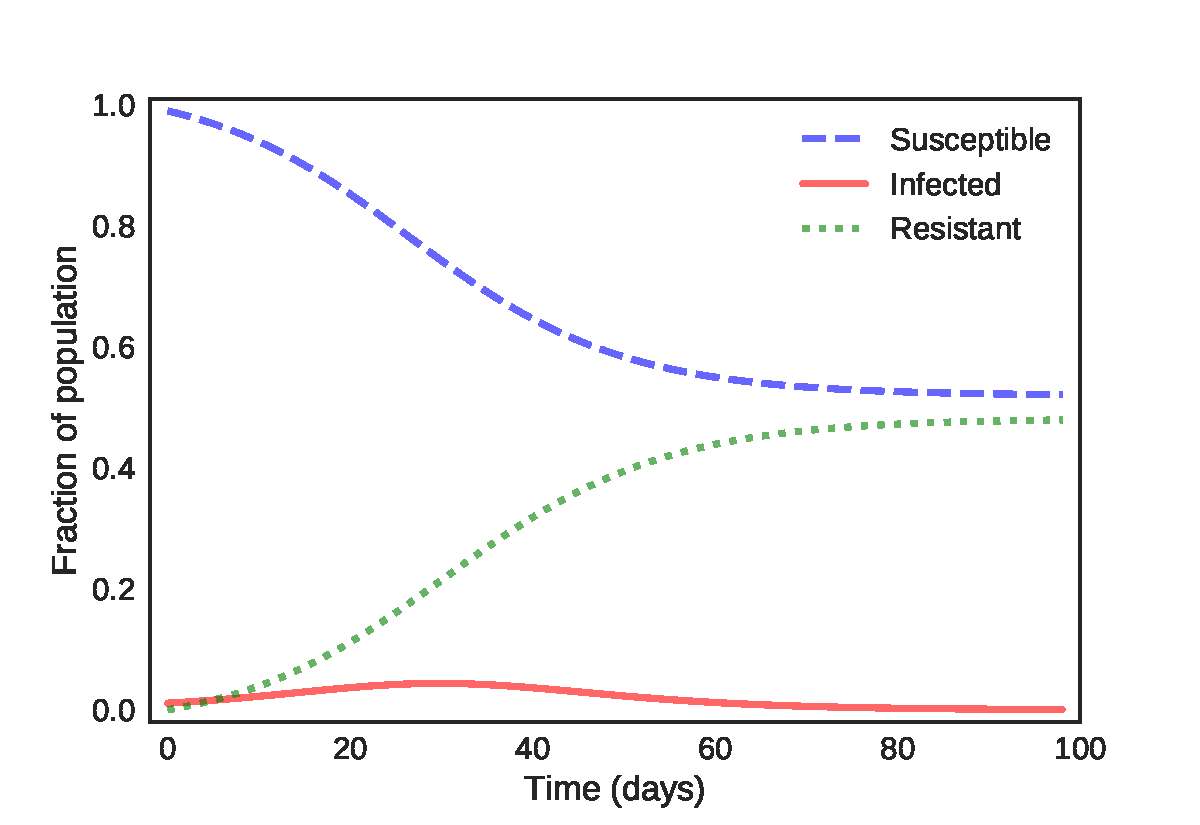
\includegraphics[height=3in]{figs/chap05-fig01.pdf}}
\caption{Estimates of world population, 1950--2016.}
\label{chap05-fig01}
\end{figure}

Figure~\ref{chap05-fig01} shows the result.  The lines overlap almost completely; for most dates the difference between the two estimates is less than 1\%.


\section{Constant growth model}

Suppose we want to predict world population growth over the next 50 or 100 years.  We can do that by developing a model that describes how populations grow, fitting the model to the data we have so far, and then using the model to generate predictions.

\index{constant growth}

In the next few sections I demonstrate this process starting with simple models and gradually improving them.

\index{iterative modeling}

Although there is some curvature in the plotted estimates, it looks like world population growth has been close to linear since 1960 or so.  So we'll start with a model that has constant growth.

To fit the model to the data, we'll compute the average annual growth from 1950 to 2016.  Since the UN and Census data are so close, we'll use the Census data.

We can select a value from a \py{Series} using the bracket operator:
\index{bracket operator}
\index{operator!bracket}

\begin{python}
census[1950]
\end{python}

So we can get the total growth during the interval like this:

\begin{python}
total_growth = census[2016] - census[1950]
\end{python}

The numbers in brackets are called {\bf labels}, because they label the rows of the \py{Series} (not to be confused with the labels we saw in the previous section, which label lines in a graph).

\index{label}

In this example, the labels 2016 and 1950 are part of the data, so it would be better not to make them part of the program.  Putting values like these in the program is called {\bf hard coding}; it is considered bad practice because if the data change in the future, we have to modify the program (see \url{http://modsimpy.com/hardcode}).

\index{hard coding}

It would be better to get the first and last labels from the \py{Series} like this:

\begin{python}
t_0 = get_first_label(census)
t_end = get_last_label(census)
elapsed_time = t_end - t_0
\end{python}

\py{get_first_label} and \py{get_last_label} are defined in \py{modsim.py}; as you might have guessed, they select the first and last labels from \py{census}.
The difference between them is the elapsed time.

The ModSim library also defines \py{get_first_value} and \py{get_last_value}, which we can use to compute \py{total_growth}:

\begin{python}
p_0 = get_first_value(census)
p_end = get_last_value(census)
total_growth = p_end - p_0
\end{python}

Finally, we can compute average annual growth.

\begin{python}
annual_growth = total_growth / elapsed_time
\end{python}

The next step is to use this estimate to simulate population growth since 1950.


\section{Simulation}

Our simulation will start with the observed population in 1950, \py{p_0}, and add \py{annual_growth} each year.  To store the results, we'll use a \py{TimeSeries} object:

\index{TimeSeries}

\begin{python}
results = TimeSeries()
\end{python}

We can set the first value in the new \py{TimeSeries} by copying the first value from \py{census}:

\begin{python}
results[t_0] = census[p_0]
\end{python}

Then we set the rest of the values by simulating annual growth:

\begin{python}
for t in linrange(t_0, t_end):
    results[t+1] = results[t] + annual_growth
\end{python}

\py{linrange} is defined in the ModSim library.  In this example it returns a NumPy array of integers from \py{t_0} to \py{t_end}, including the first but not the last.

\index{linrange}
\index{NumPy}
\index{array}

Each time through the loop, the loop variable \py{t} gets the next value from the array.  Inside the loop, we compute the population for each year by adding the population for the previous year and \py{annual_growth}.  The last time through the loop, the value of \py{t} is 2015, so the last label in \py{results} is 2016, which is what we want.

\index{loop}
\index{loop variable}

\begin{figure}
\centerline{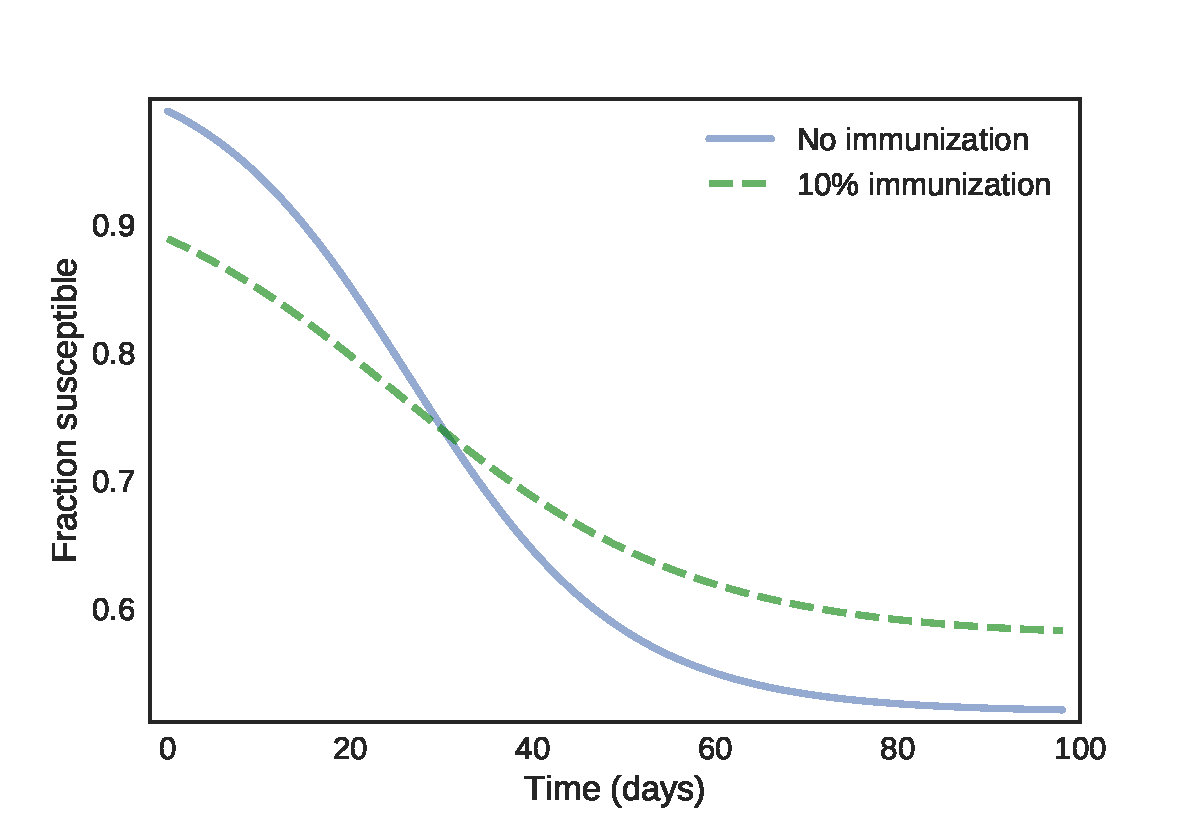
\includegraphics[height=3in]{figs/chap05-fig02.pdf}}
\caption{Estimates of world population, 1950--2016, and a constant growth model.}
\label{chap05-fig02}
\end{figure}

Figure~\ref{chap05-fig02} shows the result. The model does not fit the data particularly well from 1950 to 1990, but after that, it's pretty good.  Nevertheless, there are problems:

\begin{itemize}

\item There is no obvious mechanism that could cause population growth to be constant from year to year.  Changes in population are determined by the fraction of people who die and the fraction of people who give birth, so we expect them to depend on the current population.

\item According to this model, we would expect the population to keep growing at the same rate forever, and that does not seem reasonable.

\end{itemize}

We'll try out some different models in the next few sections, but first let's clean up the code.

Before you go on, you might want to read the notebook for this chapter, \py{chap05.ipynb}, and work on the exercises.  For instructions on downloading and running the code, see Section~\ref{code}.


\chapter{Modeling growth}
\label{chap06}
In the previous chapter we simulated a model of world population with constant growth.  In this chapter we see if we can make a better model with growth proportional to the population.

But first, we can improve the code from the previous chapter by encapsulating it in a function and using \py{System} objects.

\section{System objects}
\label{nowwithsystem}

Like a \py{State} object, a \py{System} object contains variables and their values.  The difference is:

\begin{itemize}

\item \py{State} objects contain state variables, which represent the state of the system, which get updated in the course of a simulation.

\item \py{System} objects contain {\bf system variables}, which represent parameters of the system, which usually don't get updated over the course of a simulation.

\end{itemize}  

For example, in the bike share model, state variables include the number of bikes at each location, which get updated whenever a customer moves a bike.  System variables include the number of locations, total number of bikes, and arrival rates at each location.

In the population model, the only state variable is the population.  System variables include the annual growth rate, the initial time and population, and the end time.

Suppose we have the following variables, as computed in the previous chapter (assuming that \py{census} is a \py{Series} object):

\begin{python}
t_0 = get_first_label(census)
t_end = get_last_label(census)
elapsed_time = t_end - t_0

p_0 = get_first_value(census)
p_end = get_last_value(census)
total_growth = p_end - p_0

annual_growth = total_growth / elapsed_time
\end{python}

Some of these are parameters we need to simulate the system; others are temporary values we can discard.  We can put the parameters we need into a \py{System} object like this:

\index{System object}

\begin{python}
system = System(t_0=t_0, 
                t_end=t_end,
                p_0=p_0,
                annual_growth=annual_growth)
\end{python}

\py{t0} and \py{t_end} are the first and last years; \py{p_0} is the initial population, and \py{annual_growth} is the estimated annual growth.

Next we'll wrap the code from the previous chapter in a function:

\begin{python}
def run_simulation1(system):
    results = TimeSeries()
    results[system.t_0] = system.p_0
    
    for t in linrange(system.t_0, system.t_end):
        results[t+1] = results[t] + system.annual_growth
    
    return results
\end{python}

When \py{run_simulation1} runs, it stores the results in a \py{TimeSeries} and returns it.
 
\index{TimeSeries object}

The following function plots the results along with the estimates \py{census} and \py{un}:

\begin{python}
def plot_results(census, un, timeseries, title):
    plot(census, ':', label='US Census')
    plot(un, '--', label='UN DESA')
    plot(timeseries, color='gray', label='model')
    
    decorate(xlabel='Year', 
             ylabel='World population (billion)',
             title=title)
\end{python}

\index{plot}
\index{decorate}

The \py{color} argument specifies the color of the line.  For details on color specification in Pyplot, see \url{http://modsimpy.com/color}.

\index{Pyplot}
\index{color}

Finally, we can run the simulation like this.

\begin{python}
results = run_simulation1(system)
plot_results(census, un, results, 'Constant growth model')
\end{python}

The results are the same as Figure~\ref{chap05-fig02}.

It might not be obvious that using functions and \py{System} objects is a big improvement, and for a simple model that we run only once, maybe it's not.  But as we work with more complex models, and when we run many simulations with different parameters, we'll see that the organization of the code makes a big difference.

Now let's see if we can improve the model.


\section{Proportional growth model}

The biggest problem with the constant growth model is that it doesn't make any sense.  It is hard to imagine how people all over the world could conspire to keep population growth constant from year to year.

\index{proportional growth}

On the other hand, if some fraction of the population dies each year, and some fraction gives birth, we can compute the net change in the population like this:

\begin{python}
def run_simulation2(system):
    results = TimeSeries()
    results[system.t_0] = system.p_0
    
    for t in linrange(system.t_0, system.t_end):
        births = system.birth_rate * results[t]
        deaths = system.death_rate * results[t]
        results[t+1] = results[t] + births - deaths
        
    return results
\end{python}

Now we can choose the values of \py{birth_rate} and \py{death_rate} that best fit the data.  Without trying too hard, I chose:

\begin{python}
system.death_rate = 0.01
system.birth_rate = 0.027
\end{python}

Then I ran the simulation and plotted the results:

\begin{python}
results = run_simulation2(system)
plot_results(census, un, results, 'Proportional model')
\end{python}

\begin{figure}
\centerline{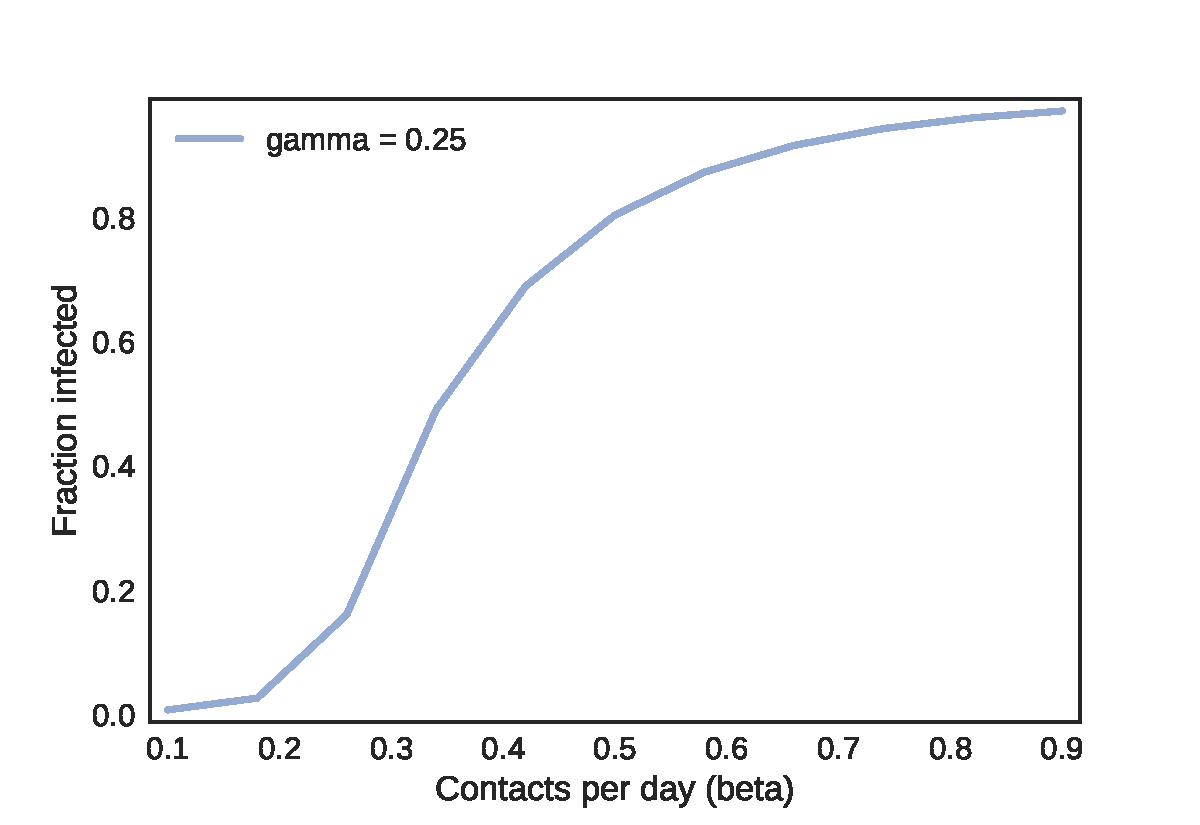
\includegraphics[height=3in]{figs/chap06-fig01.pdf}}
\caption{Estimates of world population, 1950--2016, and a proportional model.}
\label{chap06-fig01}
\end{figure}

Figure~\ref{chap06-fig01} shows the results.  The proportional model fits the data well from 1950 to 1965, but not so well after that.  Overall, the {\bf quality of fit} is not as good as the constant growth model, which is surprising, because it seems like the proportional model is more realistic.

In the next chapter we'll try one more time to find a model that makes sense and fits the data.  But first, I want to make a few more improvements to the code.


\section{Factoring out the update function}

\py{run_simulation1} and \py{run_simulation2} are nearly identical except for the body of the \py{for} loop, where we compute the population for the next year.

\index{update function}
\index{function!update}

Rather than repeat identical code, we can separate the things that change from the things that don't.  First, I'll pull out the update code from \py{run_simulation2} and make it a function:

\begin{python}
def update_func1(pop, t, system):
    births = system.birth_rate * pop
    deaths = system.death_rate * pop
    return pop + births - deaths
\end{python}

This function takes as arguments the current population, current year, and a \py{System} object; it returns the computed population for the next year.

This update function does not use \py{t}, so we could leave it out.  But we will see other functions that need it, and it is convenient if they all take the same parameters, used or not.

Now we can write a function that runs any model:

\begin{python}
def run_simulation(system, update_func):
    results = TimeSeries()
    results[system.t_0] = system.p_0
    
    for t in linrange(system.t_0, system.t_end):
        results[t+1] = update_func(results[t], t, system)
        
    return results
\end{python}

This function demonstrates a feature we have not seen before: it takes a function as a parameter!  When we call \py{run_simulation}, the second parameter is a function, like \py{update_func1}, that computes the population for the next year.

\index{function!as parameter}

Here's how we call it:

\begin{python}
results = run_simulation(system, update_func1)
\end{python}

Passing a function as an argument is the same as passing any other value.  The argument, which is \py{update_func1} in this example, gets assigned to the parameter, which is called \py{update_func}.  Inside \py{run_simulation}, we can run \py{update_func} just like any other function.

The loop in \py{run_simulation} calls \py{update_func1} once for each year between \py{t_0} and \py{t_end-1}.  The result is the same as Figure~\ref{chap06-fig01}.


\section{Combining birth and death}

While we are at it, we can also simplify the code by combining births and deaths to compute the net growth rate.  Instead of two parameters, \py{birth_rate} and \py{death_rate}, we can write the update function in terms of a single parameter that represents the difference:

\begin{python}
system.alpha = system.birth_rate - system.death_rate
\end{python}

The name of this parameter, \py{alpha}, is the conventional name for a proportional growth rate.

Here's the modified version of \py{update_func1}:

\begin{python}
def update_func2(pop, t, system):
    net_growth = system.alpha  * pop
    return pop + net_growth
\end{python}

And here's how we run it:

\begin{python}
results = run_simulation(system, update_func2)
\end{python}

Again, the result is the same as Figure~\ref{chap06-fig01}.

Before you go on, you might want to read the notebook for this chapter, \py{chap06.ipynb}, and work on the exercises.  For instructions on downloading and running the code, see Section~\ref{code}.



\chapter{Quadratic growth}
\label{chap07}

In the previous chapter we developed a population model where net growth during each time step is proportional to the current population.  This model seems more realistic than the constant growth model, but it does not fit the data as well.

There are a few things we could try to improve the model:

\begin{itemize}

\item Maybe the net growth rate varies over time.

\item Maybe net growth depends on the current population, but the relationship is quadratic, not linear.

\end{itemize}

In the notebook for this chapter, you will have a chance to try the first option.  In this chapter, we explore the second.


\section{Quadratic growth}
\label{quadratic}

It makes sense that net growth should depend on the current population, but maybe it's not a linear relationship, like this:

\begin{python}
    net_growth = system.alpha * pop
\end{python}

Maybe it's a quadratic relationship, like this:

\index{quadratic growth}

\begin{python}
    net_growth = system.alpha * pop + system.beta * pop**2
\end{python}

We can test that conjecture with a new update function:

\begin{python}
def update_func_quad(pop, t, system):
    net_growth = system.alpha * pop + system.beta * pop**2
    return pop + net_growth
\end{python}

Now we need two parameters.  I chose the following values by trial and error; we will see better ways to do it later.

\index{parameter}

\begin{python}
system.alpha = 0.025
system.beta = -0.0018
\end{python}

And here's how we run it:

\begin{python}
results = run_simulation(system, update_func_quad)
\end{python}

\begin{figure}
\centerline{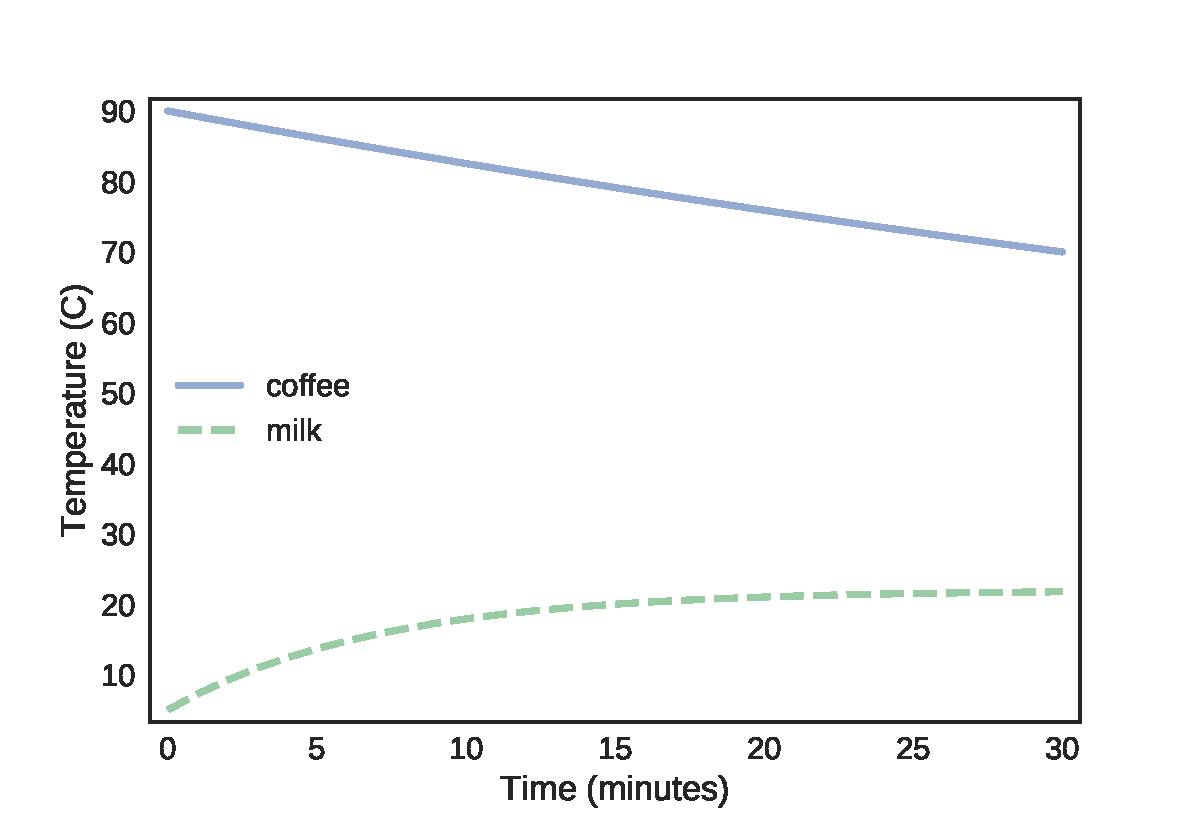
\includegraphics[height=3in]{figs/chap07-fig01.pdf}}
\caption{Estimates of world population, 1950--2016, and a quadratic model.}
\label{chap07-fig01}
\end{figure}

Figure~\ref{chap07-fig01} shows the result.  The model fits the data well over the whole range, with just a bit of space between them in the 1960s.

Of course, we should expect the quadratic model to fit better than the constant and proportional models because it has two parameters we can choose, where the other models have only one.  In general, the more parameters you have to play with, the better you should expect the model to fit.

\index{quality of fit}
\index{data}
\index{fitting data}

But fitting the data is not the only reason to think the quadratic model might be a good choice.  It also makes sense; that is, there is a legitimate reason to expect the relationship between growth and population to have this form.

To understand it, let's look at net growth as a function of population.  Here's how we compute it:

\begin{python}
pop_array = linspace(0, 15, 100)
net_growth_array = (system.alpha * pop_array + 
                    system.beta * pop_array**2)
\end{python}

\py{pop_array} contains 100 equally spaced values from 0 to 15.  \py{net_growth_array} contains the corresponding 100 values of net growth.  We can plot the results like this: 

\begin{python}
plot(pop_array, net_growth_array)
\end{python}

Previously we have used \py{plot} with \py{Series} objects.  In this example, we use two NumPy arrays, corresponding to the x and y axes.

\begin{figure}
\centerline{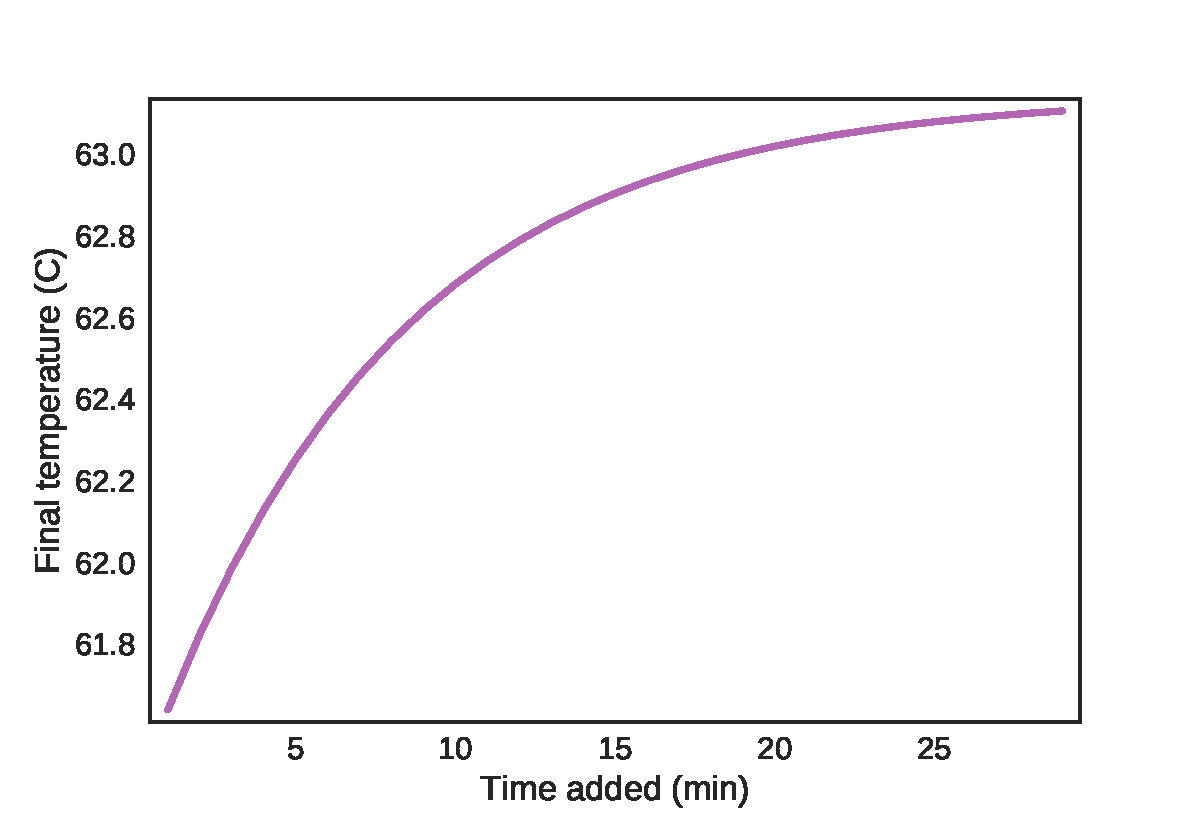
\includegraphics[height=3in]{figs/chap07-fig02.pdf}}
\caption{Net growth as a function of population.}
\label{chap07-fig02}
\end{figure}

Figure~\ref{chap07-fig02} shows the result.  Note that the x-axis is not time, as in the previous figures, but population.  We can divide this curve into four regimes of behavior:
\index{regime}

\begin{itemize}

\item When the population is less than 3-4 billion, net growth is proportional to population, as in the proportional model.  In this regime,  the population grows slowly because the population is small.

\item Between 4 billion and 10 billion, the population grows quickly because there are a lot of people.

\item Above 10 billion, population grows more slowly; this behavior models the effect of resource limitations that lower birth rates or increase death rates.

\item Above 14 billion, resources are so limited that the death rate exceeds the birth rate and net growth becomes negative.

\end{itemize}

Just below 14 billion, there is a point where net growth is 0, which means that the population does not change.  At this point, the birth and death rates are equal, so the population is in {\bf equilibrium}.

\index{equilibrium}


\section{Equilibrium}
\label{equilibrium}

To find the equilibrium point, we can find the roots, or zeros, of this equation:
%
\[ \Delta p = \alpha p + \beta p^2 \]
%
where $\Delta p$ is net population growth, $p$ is current population, and $\alpha$ and $\beta$ are the parameters of the model.  We can rewrite the right hand side like this:
%
\[ \Delta p = p (\alpha + \beta p) \]
%
which is $0$ when $p=0$ or $p=-\alpha/\beta$.  In this example, $\alpha = 0.025$ and $\beta = -0.0018$, so $-\alpha/\beta = 13.9$.

In the context of population modeling, the quadratic model is more conventionally written like this:
%
\[ \Delta p = r p (1 - p / K) \]
%
This is the same model; it's just a different way to {\bf parameterize} it.  Given $\alpha$ and $\beta$, we can compute $r=\alpha$ and $K=-\alpha/\beta$.

\index{parameterize}

In this version, it is easier to interpret the parameters: $r$ is the maximum growth rate, observed when $p$ is small, and $K$ is the equilibrium point.  $K$ is also called the {\bf carrying capacity}, since it indicates the maximum population the environment can sustain.

\index{carrying capacity}

In the next chapter we use the models we have developed to generate predictions.

\section{Dysfunctions}

When people learn about functions, there are a few things they often find confusing.  In this section I present and explain some common problems.

As an example, suppose you want a function that takes as a parameter \py{System} object with variables \py{alpha} and \py{beta}, and computes the carrying capacity, \py{-alpha/beta}.  Here's a good solution: 

\begin{python}
def carrying_capacity(system):
    K = -system.alpha / system.beta
    return K
    
sys1 = System(alpha=0.025, beta=-0.0018)
pop = carrying_capacity(sys1)
print(pop)
\end{python}

Now let's see all the ways that can go wrong.

Dysfunction \#1: Not using parameters.  In the following version, the function doesn't take any parameters; when \py{sys1} appears inside the function, it refers to the object we create outside the function.

\begin{python}
def carrying_capacity():
    K = -sys1.alpha / sys1.beta
    return K
    
sys1 = System(alpha=0.025, beta=-0.0018)
pop = carrying_capacity()
print(pop)
\end{python}

This version actually works, but it is not as versatile as it could be.  If there are several \py{System} objects, this function can only work with one of them, and only if it is named \py{sys1}.

Dysfunction \#2: Clobbering the parameters.  When people first learn about parameters, they often write functions like this:

\begin{python}
# WRONG
def carrying_capacity(system):
    system = System(alpha=0.025, beta=-0.0018)
    K = -system.alpha / system.beta
    return K
    
sys1 = System(alpha=0.03, beta=-0.002)
pop = carrying_capacity(sys1)
print(pop)
\end{python}

In this example, we have a \py{System} object named \py{sys1} that gets passed as an argument to \py{carrying_capacity}.  But when the function runs, it ignores the argument and immediately replaces it with a new \py{System} object.  As a result, this function always returns the same value, no matter what argument is passed.

When you write a function, you generally don't know what the values of the parameters will be.  Your job is to write a function that works for any valid values.  If you assign your own values to the parameters, you defeat the whole purpose of functions.


Dysfunction \#3: No return value.  Here's a version that computes the value of \py{K} but doesn't return it.

\begin{python}
# WRONG
def carrying_capacity(system):
    K = -system.alpha / system.beta
    
sys1 = System(alpha=0.025, beta=-0.0018)
pop = carrying_capacity(sys1)
print(pop)
\end{python}

A function that doesn't have a return statement always returns a special value called \py{None}, so in this example the value of \py{pop} is \py{None}.  If you are debugging a program and find that the value of a variable is \py{None} when it shouldn't be, a function without a return statement is a likely cause.
\index{None}

Dysfunction \#4: Ignoring the return value.  Finally, here's a version where the function is correct, but the way it's used is not.

\begin{python}
# WRONG
def carrying_capacity(system):
    K = -system.alpha / system.beta
    return K
    
sys1 = System(alpha=0.025, beta=-0.0018)
carrying_capacity(sys1)
print(K)
\end{python}

In this example, \py{carrying_capacity} runs and returns \py{K}, but the return value is dropped.

When you call a function that returns a value, you should do something with the result.  Often you assign it to a variable, as in the previous examples, but you can also use it as part of an expression.  For example, you could eliminate the temporary variable \py{pop} like this:

\begin{python}
print(carrying_capacity(sys1))
\end{python}

Or if you had more than one system, you could compute the total carrying capacity like this:

\begin{python}
total = carrying_capacity(sys1) + carrying_capacity(sys2)
\end{python}

Before you go on, you might want to read the notebook for this chapter, \py{chap07.ipynb}, and work on the exercises.  For instructions on downloading and running the code, see Section~\ref{code}.




\chapter{Prediction}
\label{chap08}

In the previous chapter we developed a quadratic model of world population growth from 1950 to 2016.  It is a simple model, but it fits the data well and the mechanisms it's based on are plausible.  

In this chapter we'll use the quadratic model to generate projections of future growth, and compare our results to projections from actual demographers.  Also, we'll represent the models from the previous chapters as differential equations and solve them analytically.

\index{prediction}
\index{projection}


\section{Generating projections}

We'll start with the quadratic model from Section~\ref{quadratic}, which is based on this update function:
\index{quadratic growth}

\begin{python}
def update_func_quad(pop, t, system):
    net_growth = system.alpha * pop + system.beta * pop**2
    return pop + net_growth
\end{python}

As we saw in the previous chapter, we can get the start date, end date, and initial population from \py{census}, which is a series that contains world population estimates generated by the U.S. Census:

\begin{python}
t_0 = get_first_label(census)
t_end = get_last_label(census)
p_0 = census[t_0]
\end{python}

Now we can create a \py{System} object:
\index{System object}

\begin{python}
system = System(t_0=t_0, 
                t_end=t_end,
                p_0=p_0,
                alpha=0.025,
                beta=-0.0018)
\end{python}

And run the model:

\begin{python}
results = run_simulation(system, update_func_quad)
\end{python}

We have already seen the results in Figure~\ref{chap07-fig01}.  Now, to generate a projection, the only thing we have to change is \py{t_end}:

\begin{python}
system.t_end = 2250
results = run_simulation(system, update_func_quad)
\end{python}

\begin{figure}
\centerline{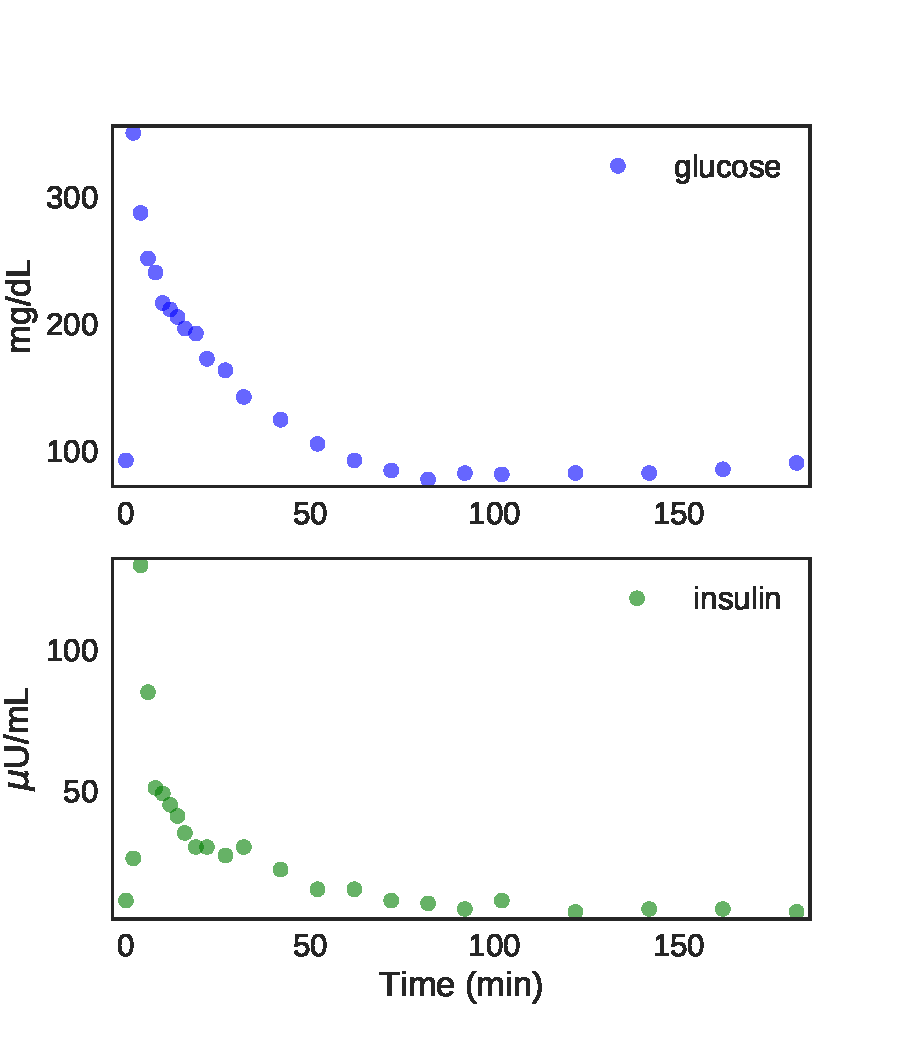
\includegraphics[height=3in]{figs/chap08-fig01.pdf}}
\caption{Quadratic model of world population growth, with projection from 2016 to 2250.}
\label{chap08-fig01}
\end{figure}

Figure~\ref{chap08-fig01} shows the result, with a projection until 2250.  According to this model, population growth will continue almost linearly for the next 50--100 years, then slow over the following 100 years, approaching 13.9 billion by 2250.

I am using the word ``projection" deliberately, rather than ``prediction", with the following distinction: ``prediction" implies something like ``this is what we should reasonably expect to happen, at least approximately"; ``projection" implies something like ``if this model is actually a good description of what is happening in this system, and if nothing in the future causes the parameters of the model to change, this is what would happen."

Using ``projection" leaves open the possibility that there are important things in the real world that are not captured in the model.  It also suggests that, even if the model is good, the parameters we estimate based on the past might be different in the future.

The quadratic model we've been working with is based on the assumption that population growth is limited by the availability of resources; in that scenario, as the population approaches carrying capacity, birth rates fall and death rates rise because resources become scarce.

\index{carrying capacity}

If that assumption is valid, we might be able to use actual population growth to estimate carrying capacity, especially if we observe the transition into the regime where the growth rate starts to fall.

But in the case of world population growth, those conditions don't apply.  Over the last 50 years, the net growth rate has leveled off, but not yet started to fall, so we don't have enough data to make a credible estimate of carrying capacity.  And resource limitations are probably {\em not} the primary reason growth has slowed.  As evidence, consider:

\begin{itemize}

\item First, the death rate is not increasing; rather, it has declined from 1.9\% in 1950 to 0.8\% now (see \url{http://modsimpy.com/mortality}).  So the decrease in net growth is due entirely to declining birth rates.

\index{mortality rate}

\item Second, the relationship between resources and birth rate is the opposite of what the model assumes; as nations develop and people become more wealthy, birth rates tend to fall.  

\index{birth rate}

\end{itemize} 

We should not take too seriously the idea that this model can estimate carrying capacity.  But the predictions of a model can be credible even if the assumptions of the model are not strictly true.  For example, population growth might behave {\em as if} it is resource limited, even if the actual mechanism is something else.

In fact, demographers who study population growth often use models similar to ours.  In the next section, we'll compare our projections to theirs.


\section{Comparing projections}

Table 3 from \url{http://modsimpy.com/worldpop} contains projections from the U.S. Census and the United Nations DESA:

\begin{python}
table3 = tables[3]
\end{python}

For some years, one agency or the other has not published a projection, so some elements of \py{table3} contain the special value \py{NaN}, which stands for ``not a number".  \py{NaN} is often used to indicate missing data.

\index{not a number}
\index{NaN}
\index{missing data}

\begin{figure}
\centerline{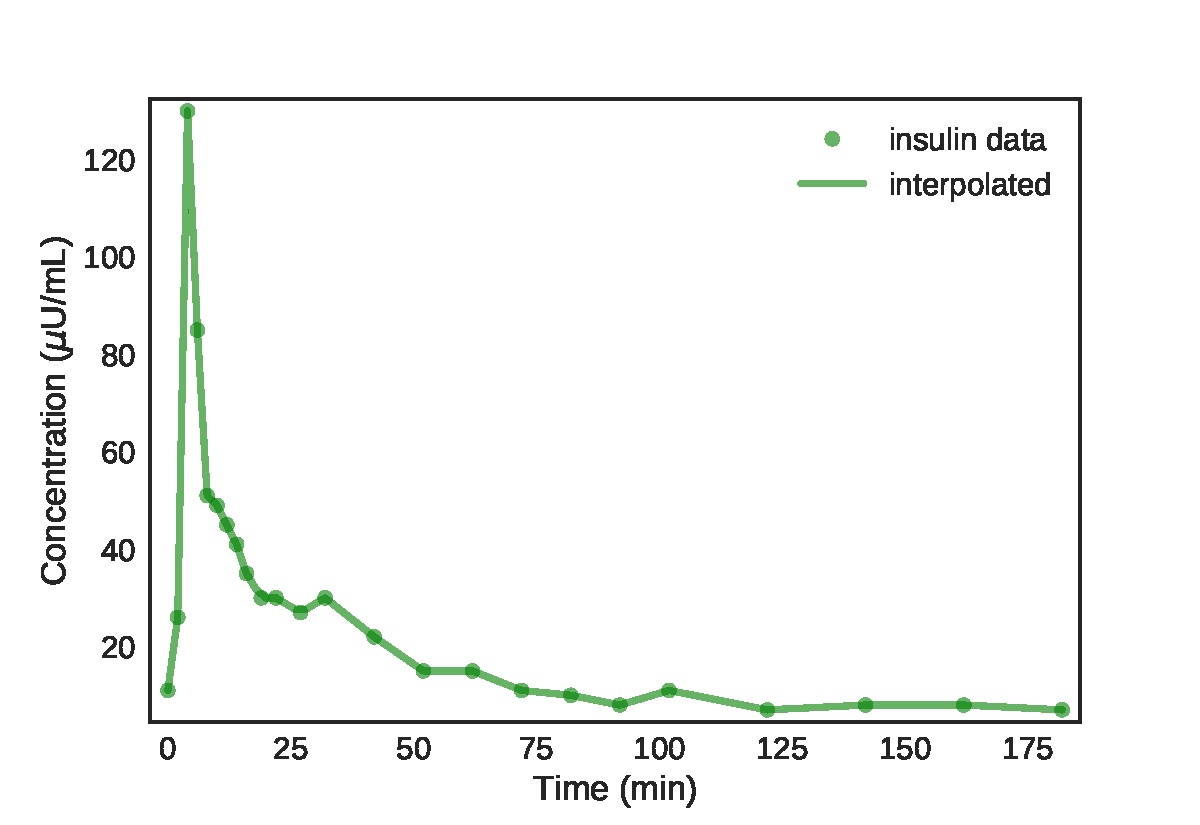
\includegraphics[height=3in]{figs/chap08-fig02.pdf}}
\caption{Projections of world population generated by the U.S. Census Bureau, the United Nations, and our quadratic model.}
\label{chap08-fig02}
\end{figure}

Pandas provides functions that deal with missing data, including \py{dropna}, which removes any elements in a series that contain \py{NaN}.  Using \py{dropna}, we can plot the projections like this:

\index{Pandas}
\index{dropna}

\begin{python}
def plot_projections(table):
    census_proj = table.census / 1e9
    un_proj = table.un / 1e9
    
    plot(census_proj.dropna(), 'b:', label='US Census')
    plot(un_proj.dropna(), 'g--', label='UN DESA')
\end{python}

The format string \py{'b:'} indicates a blue dotted line; \py{g--} indicates a green dashed line.

\index{format string}
\index{plot}

We can run our model over the same interval:

\begin{python}
system.t_end = 2100
results = run_simulation(system, update_func_quad)
\end{python}

And compare our projections to theirs.  Figure~\ref{chap08-fig02} shows the results.  Real demographers expect world population to grow more slowly than our model projects, probably because their models are broken down by region and country, where conditions are different, and they take into account expected economic development.

\index{demography}

Nevertheless, their projections are qualitatively similar to ours, and theirs differ from each other almost as much as they differ from ours.  So the results from this model, simple as it is, are not entirely crazy.

Before you go on, you might want to read the notebook for this chapter, \py{chap08.ipynb}, and work on the exercises.  For instructions on downloading and running the code, see Section~\ref{code}.


\chapter{Analysis}
\label{chap09}

In this chapter we express the models from previous chapters as difference equations and differential equations, solve the equations, and derive the functional forms of the solutions.  We also discuss the complementary roles of mathematical analysis and simulation.


\section{Recurrence relations}

The population models in the previous chapter and this one are simple enough that we didn't really need to run simulations.  We could have solved them mathematically.  For example, we wrote the constant growth model like this:

\begin{python}
model[t+1] = model[t] + annual_growth
\end{python}

In mathematical notation, we would write the same model like this:
%
\[ x_{n+1} = x_n + c \]
%
where $x_n$ is the population during year $n$, $x_0$ is a given initial population, and $c$ is constant annual growth.  This way of representing the model is a {\bf recurrence relation}; see \url{http://modsimpy.com/recur}.

\index{recurrence relation}

Sometimes it is possible to solve a recurrence relation by writing an equation that computes $x_n$, for a given value of $n$, directly; that is, without computing the intervening values from $x_1$ through $x_{n-1}$.

In the case of constant growth we can see that $x_1 = x_0 + c$, and $x_2 = x_1 + c$.  Combining these, we get $x_2 = x_0 + 2c$, then $x_3 = x_0 + 3c$, and it is not hard to conclude that in general
%
\[ x_n = x_0 + nc \]
%
So if we want to know $x_{100}$ and we don't care about the other values, we can compute it with one multiplication and one addition.

We can also write the proportional model as a recurrence relation:
%
\[ x_{n+1} = x_n + \alpha x_n \]
%
Or more conventionally as:
%
\[ x_{n+1} = x_n (1 + \alpha) \]
%
Now we can see that $x_1 = x_0 (1 + \alpha)$, and $x_2 = x_0 (1 + \alpha)^2$, and in general
%
\[ x_n = x_0 (1 + \alpha)^n \]
%
This result is a {\bf geometric progression}; see \url{http://modsimpy.com/geom}.  When $\alpha$ is positive, the factor $1+\alpha$ is greater than 1, so the elements of the sequence grow without bound.

\index{geometric progression}
\index{quadratic growth}

Finally, we can write the quadratic model like this:
%
\[ x_{n+1} = x_n + \alpha x_n + \beta x_n^2 \]
%
or with the more conventional parameterization like this:
%
\[ x_{n+1} = x_n + r x_n (1 - x_n / K) \]
%
There is no analytic solution to this equation, but we can approximate it with a differential equation and solve that, which is what we'll do in the next section.


\section{Differential equations}
\label{diffeq}

Starting again with the constant growth model
%
\[ x_{n+1} = x_n + c \]
%
If we define $\Delta x$ to be the change in $x$ from one time step to the next, we can write:
%
\[ \Delta x = x_{n+1} - x_n = c \]
%
If we define $\Delta t$ to be the time step, which is one year in the example, we can write the rate of change per unit of time like this:
%
\[ \frac{\Delta x}{\Delta t} = c \]
%
This model is {\bf discrete}, which means it is only defined at integer values of $n$ and not in between.  But in reality, people are born and die all the time, not once a year, so a {\bf continuous} model might be more realistic.

\index{discrete}
\index{continuous}
\index{time step}

We can make this model continuous by writing the rate of change in the form of a derivative:
%
\[ \frac{dx}{dt} = c \]
%
This way of representing the model is a {\bf differential equation}; see \url{http://modsimpy.com/diffeq}.

\index{differential equation}

We can solve this differential equation if we multiply both sides by $dt$:
%
\[ dx = c dt \]
%
And then integrate both sides:
%
\[ x(t) = c t + x_0 \]
%
Similarly, we can write the proportional growth model like this:
%
\[ \frac{\Delta x}{\Delta t} = \alpha x \]
%
And as a differential equation like this:
%
\[ \frac{dx}{dt} = \alpha x \]
%
If we multiply both sides by $dt$ and divide by $x$, we get
%
\[ \frac{1}{x}~dx = \alpha~dt \] 
%
Now we integrate both sides, yielding:
%
\[ \ln x = \alpha t + K \]
%
where $\ln$ is the natural logarithm and $K$ is the constant of integration.  Exponentiating both sides\footnote{The exponential function can be written $\exp(x)$ or $e^x$.  In this book I use the first form because it resembles the Python code. }, we have
%
\[ \exp(\ln(x)) = \exp(\alpha t + K) \]
%
which we can rewrite
%
\[ x = \exp(\alpha t) \exp(K) \]
%
Since $K$ is an arbitrary constant, $\exp(K)$ is also an arbitrary constant, so we can write
%
\[ x = C \exp(\alpha t) \]
%
where $C = \exp(K)$.  There are many solutions to this differential equation, with different values of $C$.  The particular solution we want is the one that has the value $x_0$ when $t=0$. 

When $t=0$, $x(t) = C$, so $C = x_0$ and the solution we want is
%
\[ x(t) = x_0 \exp(\alpha t) \]
%
If you would like to see this derivation done more carefully, you might like this video: \url{http://modsimpy.com/khan1}.

\index{logarithm}
\index{exponentiation}
\index{integration}
\index{constant of integration}


\section{Analysis and simulation}

Once you have designed a model, there are generally two ways to proceed: simulation and analysis.  Simulation often comes in the form of a computer program that models changes in a system over time, like births and deaths, or bikes moving from place to place.  Analysis often comes in the form of algebra; that is, symbolic manipulation using mathematical notation.

\index{analysis}
\index{algebra}
\index{symbolic manipulation}

Analysis and simulation have different capabilities and limitations.  Simulation is generally more versatile; it is easy to add and remove parts of a program and test many versions of a model, as we have done in the previous examples.

But there are several things we can do with analysis that are harder or impossible with simulations:

\begin{itemize}

\item With analysis we can sometimes compute, exactly and efficiently, a value that we could only approximate, less efficiently, with simulation.  For example, in Figure~\ref{chap07-fig02}, we can see that net growth goes to zero near 14 billion, and we could estimate carrying capacity using a numerical search algorithm (more about that later).  But with the analysis in Section~\ref{equilibrium}, we get the general result that $K=-\alpha/\beta$.

\item Analysis often provides ``computational shortcuts", that is, the ability to jump forward in time to compute the state of a system many time steps in the future without computing the intervening states.

\index{time step}

\item We can use analysis to state and prove generalizations about models; for example, we might prove that certain results will always or never occur.  With simulations, we can show examples and sometimes find counterexamples, but it is hard to write proofs.

\index{proof}

\item Analysis can provide insight into models and the systems they describe; for example, sometimes we can identify regimes of qualitatively different behavior and key parameters that control those behaviors.

\index{regime}

\end{itemize}

When people see what analysis can do, they sometimes get drunk with power, and imagine that it gives them a special ability to see past the veil of the material world and discern the laws of mathematics that govern the universe.  When they analyze a model of a physical system, they talk about ``the math behind it" as if our world is the mere shadow of a world of ideal mathematical entities\footnote{I am not making this up; see \url{http://modsimpy.com/plato}.}.

\index{Plato}

This is, of course, nonsense.  Mathematical notation is a language designed by humans for a purpose, specifically to facilitate symbolic manipulations like algebra.  Similarly, programming languages are designed  for a purpose, specifically to represent computational ideas and run programs.

\index{math notation}
\index{programming languages}

Each of these languages is good for the purposes it was designed for and less good for other purposes.  But they are often complementary, and one of the goals of this book is to show how they can be used together.


\section{Analysis with WolframAlpha}

Until recently, most analysis was done by rubbing graphite on wood pulp\footnote{Or ``rubbing the white rock on the black rock", a line I got from Woodie Flowers, who got it from Stephen Jacobsen.}, a process that is laborious and error-prone.  A useful alternative is symbolic computation.  If you have used services like WolframAlpha, you have used symbolic computation.

\index{symbolic computation}
\index{WolframAlpha}

For example, if you go to \url{https://www.wolframalpha.com/} and type

\begin{python}
df(t) / dt = alpha f(t)
\end{python}

WolframAlpha infers that \py{f(t)} is a function of \py{t} and \py{alpha} is a parameter; it classifies the query as a ``first-order linear ordinary differential equation", and reports the general solution:
%
\[ f(t) = c_1 \exp(\alpha t) \]
%
If you add a second equation to specify the initial condition:

\begin{python}
df(t) / dt = alpha f(t),  f(0) = p_0
\end{python}

WolframAlpha reports the particular solution:

\[ f(t) = p_0 \exp(\alpha t) \]

WolframAlpha is based on Mathematica, a powerful programming language designed specifically for symbolic computation.

\index{Mathematica}


\section{Analysis with SymPy}

Python has a library called SymPy that provides symbolic computation tools similar to Mathematica.  They are not as easy to use as WolframAlpha, but they have some other advantages.

\index{SymPy}

Before we can use SymPy, we have to import it:

\index{import statement}
\index{statement!import}

\begin{python}
from sympy import *
\end{python}

SymPy defines many functions, and some of them conflict with functions defined in \py{modsim} and the other libraries we're using.  To avoid these conflicts, I suggest that you do symbolic computation with SymPy in a separate notebook. 

SymPy defines a \py{Symbol} object that represents symbolic variable names, functions, and other mathematical entities.

\index{Symbol object}

The \py{symbols} function takes a string and returns \py{Symbol} objects.  So if we run this assignment:

\begin{python}
t = symbols('t')
\end{python}

Python understands that \py{t} is a symbol, not a numerical value.  If we now run

\begin{python}
expr = t + 1
\end{python}

Python doesn't try to perform numerical addition; rather, it creates a new \py{Symbol} that represents the sum of \py{t} and \py{1}.  We can evaluate the sum using \py{subs}, which substitutes a value for a symbol.  This example substitutes 2 for \py{t}:

\begin{python}
expr.subs(t, 2)
\end{python}

The result is 3.

Functions in SymPy are represented by a special kind of \py{Symbol}:

\begin{python}
f = Function('f')
\end{python}

Now if we write \py{f(t)}, we get an object that represents the evaluation of a function, $f$, at a value, $t$.  But again SymPy doesn't actually try to evaluate it.


\section{Differential equations in SymPy}

SymPy provides a function, \py{diff}, that can differentiate a function.  We can apply it to \py{f(t)} like this:

\index{differential equation}
\index{SymPy}

\begin{python}
dfdt = diff(f(t), t)
\end{python}

The result is a \py{Symbol} that represents the derivative of \py{f} with respect to \py{t}.  But again, SymPy doesn't try to compute the derivative yet.

\index{Symbol object}

To represent a differential equation, we use \py{Eq}:

\begin{python}
alpha = symbols('alpha')
eq1 = Eq(dfdt, alpha*f(t))
\end{python}

The result is an object that represents an equation, which is displayed like this:
%
\[ \frac{d}{d t} f{\left (t \right )} = \alpha f{\left (t \right )} \]
%
Now we can use \py{dsolve} to solve this differential equation:

\begin{python}
solution_eq = dsolve(eq1)
\end{python}

The result is the equation
%
\[ f{\left (t \right )} = C_{1} \exp(\alpha t) \]
%
This is the {\bf general solution}, which still contains an unspecified constant, $C_1$.  To get the {\bf particular solution} where $f(0) = p_0$, we substitute \py{p_0} for \py{C1}.  First, we have to create two more symbols:

\index{general solution}
\index{particular solution}

\begin{python}
C1, p_0 = symbols('C1 p_0')
\end{python}

Now we can perform the substitution:

\begin{python}
particular = solution_eq.subs(C1, p_0)
\end{python}

The result is 
%
\[ f{\left (t \right )} = p_{0} \exp(\alpha t) \]
%
This function is called the {\bf exponential growth curve}; see \url{http://modsimpy.com/expo}.

\index{exponential growth}


\section{Solving the quadratic growth model}

In the notebook for this chapter, you will see how to use the same tools to solve the quadratic growth model with parameters $r$ and $K$.  The general solution is
%
\[ f{\left (t \right )} = \frac{K \exp(C_{1} K + r t)}{\exp(C_{1} K + r t) - 1} \]
%
To get the particular solution where $f(0) = p_0$, we evaluate the general solution at $t=0$, which yields:
%
\[ f(0) = \frac{K \exp(C_{1} K)}{\exp(C_{1} K) - 1} \]
%
Then we set this expression equal to $p_0$ and solve for $C_1$.  The result is:
%
\[ C_1 = \frac{1}{K} \ln{\left (- \frac{p_{0}}{K - p_{0}} \right )} \]
%
Finally, we substitute this value of $C_1$ into the general solution, which yields:
%
\[ f(t) = \frac{K p_{0} \exp(r t)}{K + p_{0} \exp(r t) - p_{0}} \]
%
This function is called the {\bf logistic growth curve}; see \url{http://modsimpy.com/logistic}.  In the context of growth models, the logistic function is often written, equivalently,
%
\[ f(t) = \frac{K}{1 + A \exp(-rt)} \]
%
where $A = (K - p_0) / p_0$.

If you would like to see this differential equation solved by hand, you might like this video: \url{http://modsimpy.com/khan2}
\index{quadratic growth}
\index{logistic function}


\section{Summary}

The following tables summarize the results so far:

\begin{tabular}{l|l} 
\hline
Growth type         & Discrete (difference equation) \\ 
\hline 
Constant & linear: $x_n = p_0 + \alpha n$  \\ 
 
Proportional & geometric: $x_n = p_0(1+\alpha)^n$  \\ 

\end{tabular} 

\begin{tabular}{l|l} 
\hline
        & Continuous (differential equation) \\ 
\hline 
Constant & linear: $x(t) = p_0 + \alpha t$ \\ 
 
Proportional & exponential: $x(t) = p_0 \exp(\alpha t)$ \\ 
 
Quadratic & logistic: $x(t) = K / (1 + A\exp(-rt))$ \\ 
\end{tabular} 

What I've been calling the constant growth model is more commonly called ``linear growth" because the solution is a line.  Similarly, what I've called proportional is commonly called ``exponential", and what I've called quadratic is commonly called ``logistic".  I avoided these terms until now because they are based on results we had not derived yet.

\index{linear growth}
\index{exponential growth}
\index{logistic growth}

Before you go on, you might want to read the notebook for this chapter, \py{chap09sympy.ipynb}.  For instructions on downloading and running the code, see Section~\ref{code}.


\chapter{Case studies}
\label{chap10}

This chapter reviews the computational patterns we have seen so far and presents exercises where you can apply them.

\section{Computational tools}

In Chapter~\ref{chap01} we used Pint to define units and perform calculations with units:

\begin{code}
meter = UNITS.meter
second = UNITS.second
a = 9.8 * meter / second**2
\end{code}

In Chapter~\ref{chap02} we defined a \py{State} object that contains variables that represent the state of a system, usually changing over time:

\begin{code}
bikeshare = State(olin=10, wellesley=2)
\end{code}

We used update operators like \py{+=} and \py{-=} to change state variables.  We used \py{print} statements to display the values of variables.

We used the \py{flip} function to simulate random arrivals, and used \py{if} statements to check the results.

We learned to define new functions that take parameters:

\begin{code}
def step(p1, p2):
    if flip(p1):
        bike_to_wellesley()
        
    if flip(p2):
        bike_to_olin()
\end{code}

We used a \py{for} loop with the \py{range} function to execute the body of the loop a specified number of times.

\begin{code}
for i in range(4):
    step(p1, p2)
\end{code}

We learned to create a \py{TimeSeries} object and use it to store the value of a state variable as it changes over time:

\begin{code}
results = TimeSeries()

for i in range(10):
    step(0.3, 0.2)
    results[i] = bikeshare.olin
\end{code}

We used \py{plot} to plot the results, \py{decorate} to label the axes, and \py{savefig} to save the figure.

\begin{code}
plot(results, label='Olin')
decorate(xlabel='Time step (min)', 
         ylabel='Number of bikes')
savefig('chap01-fig01.pdf)
\end{code}

In Chapter~\ref{chap03} we used comparison operators to check for certain conditions and the \py{return} statement to end the execution of a function.

\begin{code}
def bike_to_olin(state):
    if state.wellesley == 0:
        state.wellesley_empty += 1
        return
    state.wellesley -= 1
    state.olin += 1
\end{code}

In Chapter~\ref{chap04} we wrote a version of \py{run_simulation} that uses a \py{return} statement to return a value:

\begin{code}
def run_simulation(p1, p2, num_steps):
    state = State(olin=10, wellesley=2, 
                  olin_empty=0, wellesley_empty=0)
                    
    for i in range(num_steps):
        step(state, p1, p2)
        
    return state
\end{code}

This version of \py{run_simulation} returns the final value of \py{state}, which contains metrics we can use to measure the performance of the system.

We used \py{linspace} to create a NumPy array of equally spaced values, and a \py{for} loop to loop through the array.  We used a \py{SweepSeries} to store results from a series of simulations, mapping from the value of a parameter to the value of a resulting metric.

\begin{code}
p1_array = linspace(0, 1, 11)
sweep = SweepSeries()

for p1 in p1_array:
    state = run_simulation(p1, p2, num_steps)
    sweep[p1] = state.olin_empty
\end{code}

In Chapter~\ref{chap05} we used Pandas to read data from a web page and store the results in a \py{DataFrame}.  We selected a column from the \py{DataFrame} to get a \py{Series}.

In Chapter~\ref{chap06} we created a \py{System} object to contain the parameters of the model, and defined another version of \py{run_simulation}:

\begin{code}
def run_simulation(system, update_func):
    results = TimeSeries()
    results[system.t_0] = system.p_0
    
    for t in linrange(system.t_0, system.t_end):
        results[t+1] = update_func(results[t], t, system)
        
    return results
\end{code}

This version takes a \py{System} object as a parameter, and an update function.  Instead of returning the final state of the system, it returns a \py{TimeSeries} that contains the state as it changes over time.

The update function takes the current state of the system, the time, and the \py{System} object as parameters, and returns the new state.  For example, here's the update function for the quadratic growth model.

\begin{code}
def update_func_quad(pop, t, system):
    net_growth = system.alpha * pop + system.beta * pop**2
    return pop + net_growth
\end{code}

In this example, the state of the system is a single number, \py{pop}.  Later we'll see examples where state is represented by a \py{State} object with more than one variable.

Chapter~\ref{chap07} introduces the quadratic growth model and 
Chapter~\ref{chap08} uses the model to generate predictions, but neither chapter introduces new computational tools.

Chapter~\ref{chap09} introduces SymPy, which we can use to create \py{Symbol} objects:

\begin{code}
t, alpha = symbols('t alpha')
f = Function('f')
\end{code}

Write differential equations:

\begin{code}
dfdt = diff(f(t), t)
eq1 = Eq(dfdt, alpha*f(t))
\end{code}

And solve them:

\begin{code}
solution_eq = dsolve(eq1)
\end{code}

That's a brief summary of the computational tools we have seen so far.


\section{Under the hood}
\label{dataframe}

So far we've been using \py{DataFrame} and \py{Series} objects without really understanding how they work.  In this section we'll review what we know so far and get into a little more detail.

Each \py{DataFrame} contains three objects: \py{index} is a sequence of labels for the rows, \py{columns} is a sequence of labels for the columns, and \py{values} is a NumPy array that contains the data.

In the \py{DataFrame} objects in this chapter, \py{index} contains years from 1950 to 2016, \py{columns} contains names of agencies and people that produce population estimates, and \py{values} is an array of estimates.

\begin{figure}
\centerline{\includegraphics[height=2.5in]{figs/dataframe.pdf}}
\caption{The elements that make up a \py{DataFrame} and a \py{Series}.}
\label{fig-dataframe}
\end{figure}

A \py{Series} is like a \py{DataFrame} with one column: it contains a string \py{name} that is like a column label, an index, and an array of values.

Figure~\ref{fig-dataframe} shows the elements of a \py{DataFrame} and \py{Series} graphically.

\index{type function}

To determine the types of these elements, we can use the Python function \py{type}:

\begin{code}
type(table2)
type(table2.index)
type(table2.columns)
type(table2.values)
\end{code}

The type of \py{table2} is \py{DataFrame}.  The type of \py{table2.index} is \py{Int64Index}, which is similar to a \py{Series}.

The type of \py{table2.columns} is \py{Index}, which might seem strange, because ``the" index is the sequence of row labels.  But the sequence of column labels is also a kind of index.

The type of \py{table2.values} is \py{ndarray}, which is the primary array type provided by NumPy; the name indicates that the array is ``n-dimensional"; that is, it can have an arbitrary number of dimensions.

In \py{census} or \py{un}, the index is an \py{Int64Index} object and the values are stored in an \py{ndarray}.  

In the ModSim library, the functions \py{get_first_label} and \py{get_last_label} provide a simple way to access the index of a \py{DataFrame} or \py{Series}:

\begin{code}
def get_first_label(series):
    return series.index[0]

def get_last_label(series):
    return series.index[-1]
\end{code}

In brackets, the number \py{0} selects the first label; the number \py{-1} selects the last label.

Several of the objects defined in \py{modsim} are modified versions of \py{Series} objects.  \py{State} and \py{System} objects are \py{Series} where the labels are variable names.  A \py{TimeSeries} is a \py{Series} where the labels are times, and a \py{SweepSeries} is a \py{Series} where the labels are parameter values.

Defining these objects wasn't necessary; we could do all the same things using \py{Series} objects.  But giving them different names makes the code easier to read and understand, and helps avoid certain kinds of errors (like getting two \py{Series} objects mixed up).

If you write simulations in Python in the future, you can continue using the objects in \py{modsim}, if you find them useful, or you can use Pandas objects directly.

\section{One queue or two?}

This chapter presents two cases studies that let you practice what you have learned so far.  The first case study is related to {\bf queueing theory}, which is the study of systems that involve waiting in lines, also known as ``queues".  

Suppose you are designing the checkout area for a new store.  There is enough room in the store for two checkout counters and a waiting area for customers.  You can make two lines, one for each counter, or one line that feeds both counters.

In theory, you might expect a single line to be better, but it has some practical drawbacks: in order to maintain a single line, you might have to install barriers, and customers might be put off by what seems to be a longer line, even if it moves faster.

So you'd like to check whether the single line is really better and by how much.  Simulation can help answer this question.

\begin{figure}
\centerline{\includegraphics[width=4.5in]{figs/queue.pdf}}
\caption{One queue, one server (left), one queue, two servers (middle), two queues, two servers (right).}
\label{fig-queue}
\end{figure}

Figure~\ref{fig-queue} shows the three scenarios we'll consider.  As we did in the bike share model, we'll assume that a customer is equally likely to arrive during any time step.  I'll denote this probability using the Greek letter lambda, $\lambda$, or the variable name \py{lam}.  The value of $\lambda$ probably varies from day to day, so we'll have to consider a range of possibilities.

Based on data from other stores, you know that it takes 5 minutes for a customer to check out, on average.  But checkout times are variable: most customers take less than 5 minutes, but some take substantially more.  A simple way to model this variability is to assume that when a customer is checking out, they always have the same probability of finishing during the next time step, regardless of how long they have been checking out.  I'll denote this probability using the Greek letter mu, $\mu$, or the variable name \py{mu}.

If we choose $\mu=1/5$ per minute, the average time for each checkout will be 5 minutes, which is consistent with the data.  Most people takes less than 5 minutes, but a few take substantially longer, which is probably not a bad model of the distribution in real stores.

Now we're ready to get started.  In the repository for this book, you'll find a notebook called \py{queue.ipynb} that contains some code to get you started and instructions.

As always, you should practice incremental development: write no more than one or two lines of code a time, and test as you go!




\section{Predicting salmon populations}

Each year the U.S. Atlantic Salmon Assessment Committee reports estimates of salmon populations in oceans and rivers in the northeastern United States.  The reports are useful for monitoring changes in these populations, but they generally do not include predictions.

The goal of this case study is to model year-to-year changes in population, evaluate how predictable these changes are, and estimate the probability that a particular population will increase or decrease in the next 10 years.

As an example, I use data from page 18 of the 2017 report, which provides population estimates for the Narraguagus and Sheepscot Rivers in Maine.

In the repository for this book, you'll find a notebook called \py{salmon.ipynb} that contains some code to get you started and instructions.

You should take my instructions as suggestions; if you want to try something different, please do!


\section{Tree growth}

This case study is based on ``Height-Age Curves for Planted Stands of Douglas Fir, with Adjustments for Density", a working paper by Flewelling, Collier, Gonyea, Marshall, and Turnblom.

% TODO: Add paper to GitHub \url{http://modsimpy.com/trees}

It provides ``site index curves", which are curves that show the expected height of the tallest tree in a stand of Douglas firs as a function of age, for a stand where the trees are the same age.

Depending on the quality of the site, the trees might grow more quickly or slowing.  So each curve is identified by a ``site index" that indicates the quality of the site.

\begin{figure}
\centerline{\includegraphics[height=3in]{figs/trees-fig01.pdf}}
\caption{Site index curves for tree growth.}
\label{trees-fig01}
\end{figure}

Figure~\ref{trees-fig01} shows site curves for three different site indices.
The goal of this case study is to explain the shape of these curves, that is, why trees grow the way they do.

As a starting place, let's assume that the ability of the tree to gain mass is limited by the area it exposes to sunlight, and that the growth rate (in mass) is proportional to that area.  In that case we can write:
%
$ m_{n+1} = m_n + \alpha A$
%
where $m_n$ is the mass of the at time step $n$, $A$ is the area exposed to sunlight, and $\alpha$ is an unknown growth parameter.

To get from $m$ to $A$, I'll make the additional assumption that mass is proportional to height raised to an unknown power:
%
$ m = \beta h^D $
%
where $h$ is height, $\beta$ is an unknown constant of proportionality, and $D$ is the dimension that relates height and mass.  I start by assuming $D=3$, but then revisit that assumption.

Finally, we'll assume that area is proportional to height squared:

$ A = \gamma h^2$

I specify height in feet, and choose units for mass and area so that $\beta=1$ and $\gamma=1$.  Putting all that together, we can write a difference equation for height:

$ h_{n+1}^D = h_n^D + \alpha h_n^2 $

With $D=3$, the solution to this equation is close to a straight line, which is not a bad model for the growth curves.  But the model implies that trees can grow forever, and we know that's not true.  As trees get taller, it gets harder for them to move water and nutrients against the force of gravity, and their growth slows.

We can model this effect by adding a factor to the model similar to what we saw in the logistic model of population growth.  Instead of assuming:

$ m_{n+1} = m_n + \alpha A $ 

Let's assume

$ m_{n+1} = m_n + \alpha A (1 - h / K) $

where $K$ is similar to the carrying capacity of the logistic model.  As $h$ approaches $K$, the factor $(1 - h/K)$ goes to 0, causing growth to level off.

In the repository for this book, you'll find a notebook called \py{trees.ipynb} that implements both models and uses them to fit the data.  There are no exercises in this case study; it is mostly meant as an example of what you can do with the tools we have so far, and a preview of what we will be able to do with the tools in the next few chapters.



\chapter{Epidemiology}
\label{chap11}

In this chapter, we develop a model of an epidemic as it spreads in a susceptible population, and use it to evaluate the effectiveness of possible interventions.

\index{epidemic}

My presentation of the SIR model in the next few chapters is based on an excellent article by David Smith and Lang Moore\footnote{Smith and Moore, ``The SIR Model for Spread of Disease," Journal of Online Mathematics and its Applications, December 2001, at \url{http://modsimpy.com/sir}.}.

\index{SIR model}


\section{The Freshman Plague}

Every year at Olin College, about 90 new students come to campus from around the country and the world.  Most of them arrive healthy and happy, but usually at least one brings with them some kind of infectious disease.  A few weeks later, predictably, some fraction of the incoming class comes down with what we call ``The Freshman Plague".

\index{Olin College}
\index{Freshman Plague}
\index{Kermack-McKendrick}

In this chapter we introduce a well-known model of infectious disease, the Kermack-McKendrick model, and use it to explain the progression of the disease over the course of the semester, predict the effect of possible interventions (like immunization) and design the most effective intervention campaign.

\index{disease}
\index{infection}
\index{design}

So far we have done our own modeling; that is, we've chosen physical systems, identified factors that seem important, and made decisions about how to represent them.  In this chapter we start with an existing model and reverse-engineer it.  Along the way, we consider the modeling decisions that went into it and identify its capabilities and limitations.


\section{The SIR model}
\label{sirmodel}

The Kermack-McKendrick model is a simple version of an {\bf SIR model}, so-named because it considers three categories of people:

\begin{itemize}

\item {\bf S}: People who are ``susceptible", that is, capable of contracting the disease if they come into contact with someone who is infected.

\item {\bf I}: People who are ``infectious", that is, capable of passing along the disease if they come into contact with someone susceptible.

\item {\bf R}: People who are ``recovered".  In the basic version of the model, people who have recovered are considered to be immune to reinfection.  That is a reasonable model for some diseases, but not for others, so it should be on the list of assumptions to reconsider later.

\end{itemize}

Let's think about how the number of people in each category changes over time.  Suppose we know that people with the disease are infectious for a period of 4 days, on average.  If 100 people are infectious at a particular point in time, and we ignore the particular time each one became infected, we expect about 1 out of 4 to recover on any particular day.

Putting that a different way, if the time between recoveries is 4 days, the recovery rate is about 0.25 recoveries per day, which we'll denote with the Greek letter gamma, $\gamma$, or the variable name \py{gamma}.

If the total number of people in the population is $N$, and the fraction currently infectious is $i$, the total number of recoveries we expect per day is $\gamma i N$.

\index{recovery rate}

Now let's think about the number of new infections.  Suppose we know that each susceptible person comes into contact with 1 person every 3 days, on average, in a way that would cause them to become infected if the other person is infected.  We'll denote this contact rate with the Greek letter beta, $\beta$.

\index{infection rate}

It's probably not reasonable to assume that we know $\beta$ ahead of time, but later we'll see how to estimate it based on data from previous outbreaks.

If $s$ is the fraction of the population that's susceptible, $s N$ is the number of susceptible people, $\beta s N$ is the number of contacts per day, and $\beta s i N$ is the number of those contacts where the other person is infectious.

\index{susceptible}

In summary:

\begin{itemize}

\item The number of recoveries we expect per day is $\gamma i N$; dividing by $N$ yields the fraction of the population that recovers in a day, which is $\gamma i$.

\item The number of new infections we expect per day is $\beta s i N$; dividing by $N$ yields the fraction of the population that gets infected in a day, which is $\beta s i$.

\end{itemize}

This model assumes that the population is closed; that is, no one arrives or departs, so the size of the population, $N$, is constant.


\section{The SIR equations}
\label{sireqn}

If we treat time as a continuous quantity, we can write differential equations that describe the rates of change for $s$, $i$, and $r$ (where $r$ is the fraction of the population that has recovered):
%
\begin{align*}
\frac{ds}{dt} &= -\beta s i \\
\frac{di}{dt} &= \beta s i - \gamma i\\
\frac{dr}{dt} &= \gamma i
\end{align*}
%
To avoid cluttering the equations, I leave it implied that $s$ is a function of time, $s(t)$, and likewise for $i$ and $r$.
\index{differential equation}

SIR models are examples of {\bf compartment models}, so-called because they divide the world into discrete categories, or compartments, and describe transitions from one compartment to another.  Compartments are also called {\bf stocks} and transitions between them are called {\bf flows}.

\index{compartment model}
\index{stock}
\index{flow}
\index{stock and flow diagram}

In this example, there are three stocks---susceptible, infectious, and recovered---and two flows---new infections and recoveries.  Compartment models are often represented visually using stock and flow diagrams (see \url{http://modsimpy.com/stock}).
Figure~\ref{stock_flow1} shows the stock and flow diagram for an SIR model.

\begin{figure}
\centerline{\includegraphics[width=4in]{figs/stock_flow1.pdf}}
\caption{Stock and flow diagram for an SIR model.}
\label{stock_flow1}
\end{figure}

Stocks are represented by rectangles, flows by arrows.  The widget in the middle of the arrows represents a valve that controls the rate of flow; the diagram shows the parameters that control the valves.


\section{Implementation}

For a given physical system, there are many possible models, and for a given model, there are many ways to represent it.  For example, we can represent an SIR model as a stock-and-flow diagram, as a set of differential equations, or as a Python program.  The process of representing a model in these forms is called {\bf implementation}.  In this section, we implement the SIR model in Python.

\index{implementation}

I'll represent the initial state of the system using a \py{State} object with state variables \py{S}, \py{I}, and \py{R}; they represent the fraction of the population in each compartment.

\index{System object}
\index{State object}
\index{state variable}

We can initialize the \py{State} object with the {\em number} of people in each compartment, assuming there is one infected student in a class of 90:

\begin{python}
init = State(S=89, I=1, R=0)
\end{python}

And then convert the numbers to fractions by dividing by the total:

\begin{python}
init /= sum(init)
\end{python}

For now, let's assume we know the time between contacts and time between recoveries:

\begin{python}
tc = 3             # time between contacts in days 
tr = 4             # recovery time in days
\end{python}

We can use them to compute the parameters of the model:

\begin{python}
beta = 1 / tc      # contact rate in per day
gamma = 1 / tr     # recovery rate in per day
\end{python}

Now we need a \py{System} object to store the parameters and initial conditions.  The following function takes the system parameters as function parameters and returns a new \py{System} object:

\index{\py{make_system}}

\begin{python}
def make_system(beta, gamma):
    init = State(S=89, I=1, R=0)
    init /= sum(init)

    t0 = 0
    t_end = 7 * 14

    return System(init=init, t0=t0, t_end=t_end,
                  beta=beta, gamma=gamma)
\end{python}

The default value for \py{t_end} is 14 weeks, about the length of a semester.


\section{The update function}

At any point in time, the state of the system is represented by a \py{State} object with three variables, \py{S}, \py{I} and \py{R}.  So I'll define an update function that takes as parameters a \py{State} object, the current time, and a \py{System} object:

\index{update function}
\index{function!update}
\index{time step}

\begin{python}
def update_func(state, t, system):
    s, i, r = state

    infected = system.beta * i * s    
    recovered = system.gamma * i
    
    s -= infected
    i += infected - recovered
    r += recovered
    
    return State(S=s, I=i, R=r)
\end{python}

The first line uses a feature we have not seen before, {\bf multiple assignment}.  The value on the right side is a \py{State} object that contains three values.  The left side is a sequence of three variable names.  The assignment does just what we want: it assigns the three values from the \py{State} object to the three variables, in order.

The local variables, \py{s}, \py{i} and \py{r}, are lowercase to distinguish them from the state variables, \py{S}, \py{I} and \py{R}.

\index{State object}
\index{state variable}
\index{local variable}

The update function computes \py{infected} and \py{recovered} as a fraction of the population, then updates \py{s}, \py{i} and \py{r}.  The return value is a \py{State} that contains the updated values.

\index{return value}

When we call \py{update_func} like this:

\begin{python}
state = update_func(init, 0, system)
\end{python}

The result is a \py{State} object with these values:

\begin{tabular}{lr}
 & {\bf \sf value} \\ 
\hline 
{\bf \sf S} & 0.985388 \\ 
{\bf \sf I} & 0.011865 \\ 
{\bf \sf R} & 0.002747 \\ 
\end{tabular} 

You might notice that this version of \py{update_func} does not use one of its parameters, \py{t}.  I include it anyway because update functions sometimes depend on time, and it is convenient if they all take the same parameters, whether they need them or not.

%TODO: figure out when to talk about integers and floats (or never)


\section{Running the simulation}

Now we can simulate the model over a sequence of time steps:

\index{time step}

\begin{python}
def run_simulation(system, update_func):
    state = system.init

    for t in linrange(system.t0, system.t_end):
        state = update_func(state, t, system)

    return state
\end{python}

The parameters of \py{run_simulation} are the \py{System} object and the update function.  The \py{System} object contains the parameters, initial conditions, and values of \py{t0} and \py{t_end}.

\index{\py{run_simulation}}

The outline of this function should look familiar; it is similar to the function we used for the population model in Section~\ref{nowwithsystem}.

We can call \py{run_simulation} like this:

\begin{python}
system = make_system(beta, gamma)
final_state = run_simulation(system, update_func)
\end{python}

The result is the final state of the system:

\begin{tabular}{lr}
 & {\bf \sf value} \\ 
\hline 
{\bf \sf S} & 0.520819 \\ 
{\bf \sf I} & 0.000676 \\ 
{\bf \sf R} & 0.478505 \\ 
\end{tabular} 

This result indicates that after 14 weeks (98 days), about 52\% of the population is still susceptible, which means they were never infected, less than 1\% are actively infected, and 48\% have recovered, which means they were infected at some point.


\section{Collecting the results}

The previous version of \py{run_simulation} only returns the final state, but we might want to see how the state changes over time.  We'll consider two ways to do that: first, using three \py{TimeSeries} objects, then using a new object called a \py{TimeFrame}.

\index{TimeFrame object}
\index{TimeSeries object}

Here's the first version:

\begin{python}
def run_simulation(system, update_func):
    S = TimeSeries()
    I = TimeSeries()
    R = TimeSeries()

    state = system.init
    t0 = system.t0
    S[t0], I[t0], R[t0] = state
    
    for t in linrange(system.t0, system.t_end):
        state = update_func(state, t, system)
        S[t+1], I[t+1], R[t+1] = state
    
    return S, I, R
\end{python}

First, we create \py{TimeSeries} objects to store the results.  Notice that the variables \py{S}, \py{I}, and \py{R} are \py{TimeSeries} objects now.

Next we initialize \py{state}, \py{t0}, and the first elements of \py{S}, \py{I} and \py{R}.  

Inside the loop, we use \py{update_func} to compute the state of the system at the next time step, then use multiple assignment to unpack the elements of \py{state}, assigning each to the corresponding \py{TimeSeries}.

\index{time step}

At the end of the function, we return the values \py{S}, \py{I}, and \py{R}.  This is the first example we have seen where a function returns more than one value.

Now we can run the function like this:

\begin{python}
system = make_system(beta, gamma)
S, I, R = run_simulation(system, update_func)
\end{python}

We'll use the following function to plot the results:

\begin{python}
def plot_results(S, I, R):
    plot(S, '--', label='Susceptible')
    plot(I, '-', label='Infected')
    plot(R, ':', label='Resistant')
    decorate(xlabel='Time (days)',
             ylabel='Fraction of population')
\end{python}

\index{plot}
\index{decorate}

And run it like this:

\begin{python}
plot_results(S, I, R)
\end{python}

\begin{figure}
\centerline{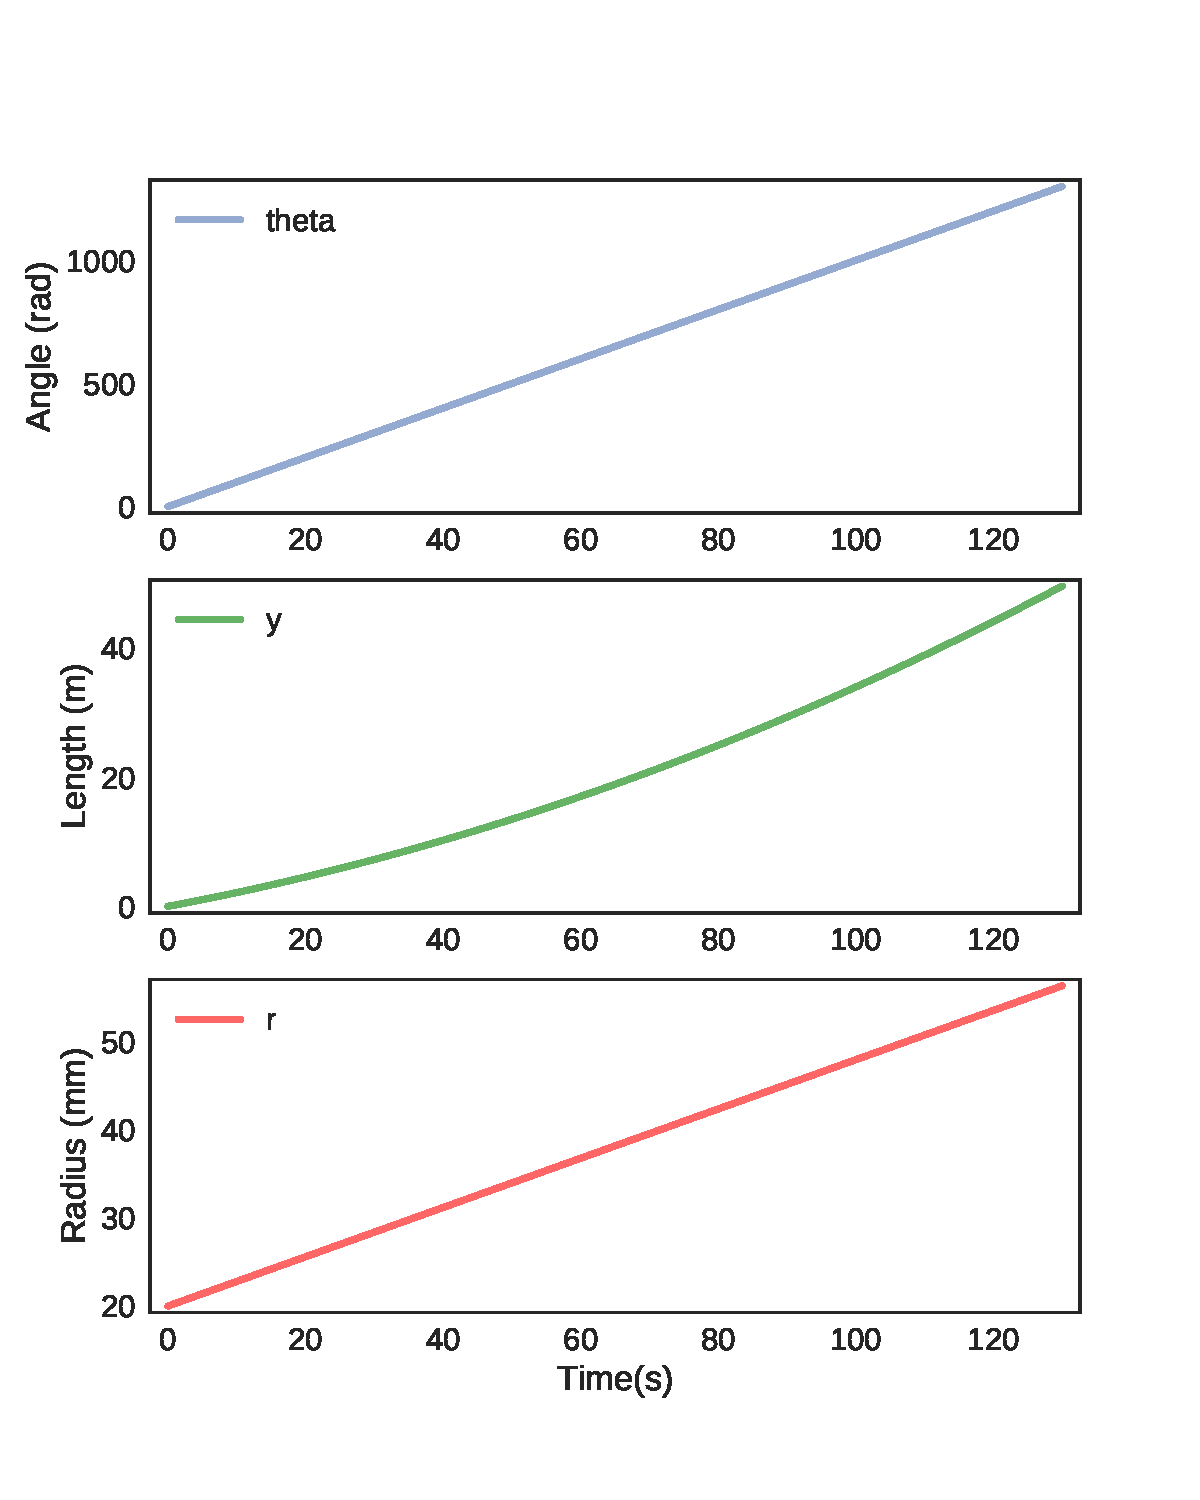
\includegraphics[height=3in]{figs/chap11-fig01.pdf}}
\caption{Time series for \py{S}, \py{I}, and \py{R} over the course of 98 days.}
\label{chap11-fig01}
\end{figure}

Figure~\ref{chap11-fig01} shows the result.  Notice that it takes about three weeks (21 days) for the outbreak to get going, and about six weeks (42 days) before it peaks.  The fraction of the population that's infected is never very high, but it adds up.  In total, almost half the population gets sick. 


\section{Now with a TimeFrame}
\label{timeframe}

If the number of state variables is small, storing them as separate \py{TimeSeries} objects might not be so bad.  But a better alternative is to use a \py{TimeFrame}, which is another object defined in the ModSim library.

\index{TimeFrame object}
\index{DataFrame object}

A \py{TimeFrame} is almost identical to a \py{DataFrame}, which we used in Section~\ref{worldpopdata}, with just a few changes I made to adapt it for our purposes.

Here's a more concise version of \py{run_simulation} using a \py{TimeFrame}:

\begin{python}
def run_simulation(system, update_func):
    frame = TimeFrame(columns=system.init.index)
    frame.row[system.t0] = system.init
    
    for t in linrange(system.t0, system.t_end):
        frame.row[t+1] = update_func(frame.row[t], system)
    
    return frame
\end{python}

The first line creates an empty \py{TimeFrame} with one column for each state variable.  Then, before the loop starts, we store the initial conditions in the \py{TimeFrame} at \py{t0}.  Based on the way we've been using \py{TimeSeries} objects, it is tempting to write:

\begin{python}
frame[system.t0] = system.init
\end{python}

But when you use the bracket operator with a \py{TimeFrame} or \py{DataFrame}, it selects a column, not a row.  For example, to select a column, we could write:

\index{bracket operator}
\index{operator~bracket}

\begin{python}
frame['S']
\end{python}

To select a row, we have to use \py{row}, like this:

\index{row}

\begin{python}
frame.row[system.t0] = system.init
\end{python}

Since the value on the right side is a \py{State}, the assignment matches up the index of the \py{State} with the columns of the \py{TimeFrame}; that is, it assigns the \py{S} value from \py{system.init} to the \py{S} column of \py{frame}, and likewise with \py{I} and \py{R}.

\index{assignment}

We can use the same feature to write the loop more concisely, assigning the \py{State} we get from \py{update_func} directly to the next row of \py{frame}.
  
\index{system variable}

Finally, we return \py{frame}.  We can call this version of \py{run_simulation} like this:

\begin{python}
results = run_simulation(system, update_func)
\end{python}

And plot the results like this:

\begin{python}
plot_results(results.S, results.I, results.R)
\end{python}

As with a \py{DataFrame}, we can use the dot operator to select columns from a \py{TimeFrame}.

\index{dot operator}
\index{operator!dot}

Before you go on, you might want to read the notebook for this chapter, \py{chap11.ipynb}, and work on the exercises.  For instructions on downloading and running the code, see Section~\ref{code}.


\chapter{Optimization}
\label{chap12}

In the previous chapter I presented the SIR model of infectious disease and used it to model the Freshman Plague at Olin.  In this chapter we'll consider metrics intended to quantify the effects of the disease and interventions intended to reduce those effects.

\section{Metrics}
\label{metrics2}

When we plot a time series, we get a view of everything that happened when the model ran, but often we want to boil it down to a few numbers that summarize the outcome.  These summary statistics are called {\bf metrics}, as we saw in Section~\ref{metrics}.

\index{metric}

In the SIR model, we might want to know the time until the peak of the outbreak, the number of people who are sick at the peak, the number of students who will still be sick at the end of the semester, or the total number of students who get sick at any point.

As an example, I will focus on the last one --- the total number of sick students --- and we will consider interventions intended to minimize it.

When a person gets infected, they move from \py{S} to \py{I}, so we can get the total number of infections by computing the difference in \py{S} at the beginning and the end:

\begin{python}
def calc_total_infected(results, system):
    return results.S[system.t0] - results.S[system.t_end]
\end{python}

In the notebook that accompanies this chapter, you will have a chance to write functions that compute other metrics.  Two functions you might find useful are \py{max} and \py{idxmax}.

\index{max}
\index{idxmax}
 
If you have a \py{Series} called \py{S}, you can compute the largest value of the series like this:

\begin{python}
largest_value = S.max()
\end{python}

And the label of the largest value like this:

\begin{python}
time_of_largest_value = S.idxmax()
\end{python}

If the \py{Series} is a \py{TimeSeries}, the label you get from \py{idxmax} is a time or date.  You can read more about these functions in the \py{Series} documentation at \url{http://modsimpy.com/series}.

\index{Series}


\section{Immunization}

Models like this are useful for testing ``what if?" scenarios.  As an example, we'll consider the effect of immunization.

\index{immunization}
\index{vaccine}
\index{Freshman Plague}

Suppose there is a vaccine that causes a student to become immune to the Freshman Plague without being infected.  How might you modify the model to capture this effect?

One option is to treat immunization as a shortcut from susceptible to recovered without going through infectious.  We can implement this feature like this:

\begin{python}
def add_immunization(system, fraction):
    system.init.S -= fraction
    system.init.R += fraction
\end{python}

\py{add_immunization} moves the given fraction of the population from \py{S} to \py{R}.  If we assume that 10\% of students are vaccinated at the beginning of the semester, and the vaccine is 100\% effective, we can simulate the effect like this:

\begin{python}
system2 = make_system(beta, gamma)
add_immunization(system2, 0.1)
results2 = run_simulation(system2, update_func)
\end{python}

For comparison, we can run the same model without immunization and plot the results.  Figure~\ref{chap12-fig01} shows \py{S} as a function of time, with and without immunization.  

\begin{figure}
\centerline{\includegraphics[height=3in]{figs/chap12-fig01.pdf}}
\caption{Time series for \py{S}, with and without immunization.}
\label{chap12-fig01}
\end{figure}

Without immunization, almost 47\% of the population gets infected at some point.  With 10\% immunization, only 31\% gets infected.  That's pretty good.

\begin{figure}
\centerline{\includegraphics[height=3in]{figs/chap12-fig02.pdf}}
\caption{Fraction of the population infected as a function of immunization rate.}
\label{chap12-fig02}
\end{figure} 

Now let's see what happens if we administer more vaccines.  This following function sweeps a range of immunization rates:

\index{sweep}

\begin{python}
def sweep_immunity(immunize_array):
    sweep = SweepSeries()

    for fraction in immunize_array:
        sir = make_system(beta, gamma)
        add_immunization(sir, fraction)
        results = run_simulation(sir, update_func)
        sweep[fraction] = calc_total_infected(results, sir)

    return sweep
\end{python}

The parameter of \py{sweep_immunity} is an array of immunization rates.  The result is a \py{SweepSeries} object that maps from each immunization rate to the resulting fraction of students ever infected.
  
\index{SweepSeries object}
\index{parameter sweep}

Figure~\ref{chap12-fig02} shows a plot of the \py{SweepSeries}.  Notice that the x-axis is the immunization rate, not time.

As the immunization rate increases, the number of infections drops steeply.  If 40\% of the students are immunized, fewer than 4\% get sick.  That's because immunization has two effects: it protects the people who get immunized (of course) but it also protects the rest of the population. 

Reducing the number of ``susceptibles" and increasing the number of ``resistants" makes it harder for the disease to spread, because some fraction of contacts are wasted on people who cannot be infected.  This phenomenon is called {\bf herd immunity}, and it is an important element of public health (see \url{http://modsimpy.com/herd}).

\index{herd immunity}

The steepness of the curve in Figure~\ref{chap12-fig02} is a blessing and a curse.  It's a blessing because it means we don't have to immunize everyone, and vaccines can protect the ``herd" even if they are not 100\% effective.

But it's a curse because a small decrease in immunization can cause a big increase in infections.  In this example, if we drop from 80\% immunization to 60\%, that might not be too bad.  But if we drop from 40\% to 20\%, that would trigger a major outbreak, affecting more than 15\% of the population.  For a serious disease like measles, just to name one, that would be a public health catastrophe.

\index{measles}

One use of models like this is to demonstrate phenomena like herd immunity and to predict the effect of interventions like vaccination.  Another use is to evaluate alternatives and guide decision making.  We'll see an example in the next section.





\section{Hand washing}

Suppose you are the Dean of Student Life, and you have a budget of just \$1200 to combat the Freshman Plague.  You have two options for spending this money:

\begin{enumerate}

\item You can pay for vaccinations, at a rate of \$100 per dose.

\item You can spend money on a campaign to remind students to wash hands frequently.

\end{enumerate}

We have already seen how we can model the effect of vaccination.  Now let's think about the hand-washing campaign.  We'll have to answer two questions:

\begin{enumerate}

\item How should we incorporate the effect of hand washing in the model?

\item How should we quantify the effect of the money we spend on a hand-washing campaign?

\end{enumerate}

For the sake of simplicity, let's assume that we have data from a similar campaign at another school showing that a well-funded campaign can change student behavior enough to reduce the infection rate by 20\%.  

In terms of the model, hand washing has the effect of reducing \py{beta}.  That's not the only way we could incorporate the effect, but it seems reasonable and it's easy to implement.

Now we have to model the relationship between the money we spend and the effectiveness of the campaign.  Again, let's suppose we have data from another school that suggests:

\begin{itemize}

\item If we spend \$500 on posters, materials, and staff time, we can change student behavior in a way that decreases the effective value of \py{beta} by 10\%.

\item If we spend \$1000, the total decrease in \py{beta} is almost 20\%.

\item Above \$1000, additional spending has little additional benefit.

\end{itemize}

In the notebook for this chapter you will see how I used a logistic curve to fit this data.  The result is the following function, which takes spending as a parameter and returns \py{factor}, which is the factor by which \py{beta} is reduced:

\index{logistic curve}

\begin{python}
def compute_factor(spending):
    return logistic(spending, M=500, K=0.2, B=0.01)
\end{python}

I use \py{compute_factor} to write \py{add_hand_washing}, which takes a \py{System} object and a budget, and modifies \py{system.beta} to model the effect of hand washing:

\begin{python}
def add_hand_washing(system, spending):
    factor = compute_factor(spending)
    system.beta *= (1 - factor)
\end{python}

Now we can sweep a range of values for \py{spending} and use the simulation to compute the effect:

\begin{python}
def sweep_hand_washing(spending_array):
    sweep = SweepSeries()
    
    for spending in spending_array:
        sir = make_system(beta, gamma)
        add_hand_washing(sir, spending)
        results, run_simulation(sir, update_func)
        sweep[spending] = calc_total_infected(results, sir)
        
    return sweep
\end{python}

Here's how we run it:

\begin{python}
spending_array = linspace(0, 1200, 20)
infected_sweep = sweep_hand_washing(spending_array)
\end{python}

\begin{figure}
\centerline{\includegraphics[height=3in]{figs/chap12-fig03.pdf}}
\caption{Fraction of the population infected as a function of hand-washing campaign spending.}
\label{chap12-fig03}
\end{figure} 

Figure~\ref{chap12-fig03} shows the result.  Below \$200, the campaign has little effect.  At \$800 it has a substantial effect, reducing total infections from 46\% to 20\%.  Above \$800, the additional benefit is small.


\section{Optimization} 

\begin{figure}
\centerline{\includegraphics[height=3in]{figs/chap12-fig04.pdf}}
\caption{Fraction of the population infected as a function of the number of doses.}
\label{chap12-fig04}
\end{figure} 

Let's put it all together.  With a fixed budget of \$1200, we have to decide how many doses of vaccine to buy and how much to spend on the hand-washing campaign.

\index{optimization}

Here are the parameters:

\begin{python}
num_students = 90
budget = 1200
price_per_dose = 100
max_doses = int(budget / price_per_dose)
\end{python}

The fraction \py{budget/price_per_dose} might not be an integer.  \py{int} is a built-in function that converts numbers to integers, rounding down.

We'll sweep the range of possible doses:

\begin{python}
dose_array = linrange(max_doses, endpoint=True)
\end{python}

In this example we call \py{linrange} with only one argument; it returns a NumPy array with the integers from 0 to \py{max_doses}.  With the argument \py{endpoint=True}, the result includes both endpoints.

\index{linrange}
\index{NumPy}
 \index{array}

Then we run the simulation for each element of \py{dose_array}:

\begin{python}
def sweep_doses(dose_array):
    sweep = SweepSeries()
    
    for doses in dose_array:
        fraction = doses / num_students
        spending = budget - doses * price_per_dose
        
        sir = make_system(beta, gamma)
        add_immunization(sir, fraction)
        add_hand_washing(sir, spending)
        
        run_simulation(sir, update_func)
        sweep[doses] = calc_total_infected(sir)

    return sweep
\end{python}

For each number of doses, we compute the fraction of students we can immunize, \py{fraction} and the remaining budget we can spend on the campaign, \py{spending}.  Then we run the simulation with those quantities and store the number of infections.

Figure~\ref{chap12-fig04} shows the result.  If we buy no doses of vaccine and spend the entire budget on the campaign, the fraction infected is around 19\%.  At 4 doses, we have \$800 left for the campaign, and this is the optimal point that minimizes the number of students who get sick.

As we increase the number of doses, we have to cut campaign spending, which turns out to make things worse.  But interestingly, when we get above 10 doses, the effect of herd immunity starts to kick in, and the number of sick students goes down again.

\index{herd immunity}

Before you go on, you might want to read the notebook for this chapter, \py{chap12.ipynb}, and work on the exercises.  For instructions on downloading and running the code, see Section~\ref{code}.



\chapter{Sweeping two parameters}
\label{chap13}

In the previous chapters I presented an SIR model of infectious disease, specifically the Kermack-McKendrick model.  We extended the model to include vaccination and the effect of a hand-washing campaign, and used the extended model to allocate a limited budget optimally, that is, to minimize the number of infections.

\index{Kermack-McKendrick model}
\index{SIR model}

But we assumed that the parameters of the model, contact rate and recovery rate, were known.  In this chapter, we explore the behavior of the model as we vary these parameters, use analysis to understand these relationships better, and propose a method for using data to estimate parameters.

\section{Sweeping beta}

Recall that $\beta$ is the contact rate, which captures both the frequency of interaction between people and the fraction of those interactions that result in a new infection.  If $N$ is the size of the population and $s$ is the fraction that's susceptible, $s N$ is the number of susceptibles, $\beta s N$ is the number of contacts per day between susceptibles and other people, and $\beta s i N$ is the number of those contacts where the other person is infectious.
\index{parameter sweep}

As $\beta$ increases, we expect the total number of infections to increase.  To quantify that relationship, I'll create a range of values for $\beta$:

\begin{python}
beta_array = linspace(0.1, 1.1, 11)
\end{python}

Then run the simulation for each value and print the results.

\begin{python}
for beta in beta_array:
    sir = make_system(beta, gamma)
    run_simulation(sir, update1)
    print(sir.beta, calc_total_infected(sir))
\end{python}

We can wrap that code in a function and store the results in a \py{SweepSeries} object:
\index{SweepSeries object}

\begin{python}
def sweep_beta(beta_array, gamma):
    sweep = SweepSeries()
    for beta in beta_array:
        system = make_system(beta, gamma)
        run_simulation(system, update1)
        sweep[system.beta] = calc_total_infected(system)
    return sweep
\end{python}

Now we can run \py{sweep_beta} like this:

\begin{python}
infected_sweep = sweep_beta(beta_array, gamma)
\end{python}

And plot the results:

\begin{python}
label = 'gamma = ' + str(gamma)
plot(infected_sweep, label=label)
\end{python}

The first line uses string operations to assemble a label for the plotted line:
\index{string}

\begin{itemize}

\item When the \py{+} operator is applied to strings, it joins them end-to-end, which is called {\bf concatenation}. 
 
\index{concatenation}

\item The function \py{str} converts any type of object to a String representation.  In this case, \py{gamma} is a number, so we have to convert it to a string before trying to concatenate it.

\index{str function}

\end{itemize}

% TODO: Make the gamma symbol appear in the line below and in the figures.

If the value of \py{gamma} is \py{0.25}, the value of \py{label} is the string \py{'gamma = 0.25'}.

\begin{figure}
\centerline{\includegraphics[height=3in]{figs/chap13-fig01.pdf}}
\caption{Fraction of students infected as a function of the parameter \py{beta}, with \py{gamma = 0.25}.}
\label{chap13-fig01}
\end{figure}

Figure~\ref{chap13-fig01} shows the results.  Remember that this figure is a parameter sweep, not a time series, so the x-axis is the parameter \py{beta}, not time.  

When \py{beta} is small, the contact rate is low and the outbreak never really takes off; the total number of infected students is near zero.  As \py{beta} increases, it reaches a threshold near 0.3 where the fraction of infected students increases quickly.  When \py{beta} exceeds 0.5, more than 80\% of the population gets sick.


\section{Sweeping gamma}

Let's see what that looks like for a few different values of \py{gamma}.  Again, we'll use \py{linspace} to make an array of values:

\index{linspace}

\begin{python}
gamma_array = linspace(0.1, 0.7, 4)
\end{python}

And run \py{sweep_beta} for each value of \py{gamma}:

\begin{python}
for gamma in gamma_array:
    infected_sweep = sweep_beta(beta_array, gamma)
    label = 'gamma = ' + str(gamma)
    plot(infected_sweep, label=label)
\end{python}

\begin{figure}
\centerline{\includegraphics[height=3in]{figs/chap13-fig02.pdf}}
\caption{Fraction of students infected as a function of the parameter \py{beta}, for several values of \py{gamma}.}
\label{chap13-fig02}
\end{figure}

Figure~\ref{chap13-fig02} shows the results.  When \py{gamma} is low, the recovery rate is low, which means people are infectious longer.  In that case, even a low contact rate (\py{beta}) results in an epidemic.

When \py{gamma} is high, \py{beta} has to be even higher to get things going.


\section{SweepFrame}
\label{sweepframe}

In the previous section, we swept a range of values for \py{gamma}, and for each value, we swept a range of values for \py{beta}.  This process is a {\bf two-dimensional sweep}.  

If we want to store the results, rather than plot them, we can use a \py{SweepFrame}, which is a kind of {\tt DataFrame} where the rows sweep one parameter, the columns sweep another parameter, and the values contain  metrics from a simulation.

\index{SweepFrame object}
\index{DataFrame object}

This function shows how it works:

\begin{python}
def sweep_parameters(beta_array, gamma_array):
    frame = SweepFrame(columns=gamma_array)
    for gamma in gamma_array:
        frame[gamma] = sweep_beta(beta_array, gamma)
    return frame
\end{python}

\py{sweep_parameters} takes as parameters an array of values for \py{beta} and an array of values for \py{gamma}.

It creates a \py{SweepFrame} to store the results, with one column for each value of \py{gamma} and one row for each value of \py{beta}.

Each time through the loop, we run \py{sweep_beta}.  The result is a \py{SweepSeries} object with one element for each value of \py{beta}.  The assignment inside the loop stores the \py{SweepSeries} as a new column in the \py{SweepFrame}, corresponding to the current value of \py{gamma}.

At the end, the \py{SweepFrame} stores the fraction of students infected for each pair of parameters, \py{beta} and \py{gamma}.

We can run \py{sweep_parameters} like this:

\begin{python}
frame = sweep_parameters(beta_array, gamma_array)
\end{python}

With the results in a \py{SweepFrame}, we can plot each column like this:

\begin{python}
for gamma in gamma_array:
    label = 'gamma = ' + str(gamma)
    plot(frame[gamma], label=label)
\end{python}

Alternatively, we can plot each row like this:

\begin{python}
for beta in [1.1, 0.9, 0.7, 0.5, 0.3]:
    label = 'β = ' + str(beta)
    plot(frame.row[beta], label=label)
\end{python}

\begin{figure}
\centerline{\includegraphics[height=3in]{figs/chap13-fig03.pdf}}
\caption{Fraction of students infected as a function of the parameter \py{gamma}, for several values of \py{beta}.}
\label{chap13-fig03}
\end{figure}

Figure~\ref{chap13-fig03} shows the results.  This example demonstrates one use of a \py{SweepFrame}: we can run the analysis once, save the results, and then generate different visualizations.

Another way to visualize the results of a two-dimensional sweep is a {\bf contour plot}, which shows the parameters on the axes and contour lines, that is, lines of constant value.  In this example, the value is the fraction of students infected.

\index{contour plot}

The ModSim library provides \py{contour}, which takes a \py{SweepFrame} as a parameter:

\begin{python}
contour(frame)
\end{python}

\begin{figure}
\centerline{\includegraphics[height=3in]{figs/chap13-fig04.pdf}}
\caption{Contour plot showing fraction of students infected as a function of the parameters \py{gamma} and \py{beta}.}
\label{chap13-fig04}
\end{figure}

Figure~\ref{chap13-fig04} shows the result.  Infection rates are lowest in the lower right, where the contact rate is and the recovery rate is high.  They increase as we move to the upper left, where the contact rate is high and the recovery rate is low.

This figure suggests that there might be a relationship between \py{beta} and \py{gamma} that determines the outcome of the model.  In fact, there is.  In the next chapter we'll explore it by running simulations, then derive it by analysis.

Before you go on, you might want to read the notebook for this chapter, \py{chap13.ipynb}, and work on the exercises.  For instructions on downloading and running the code, see Section~\ref{code}.


\chapter{Analysis} 
\label{chap14}

In the previous chapters we used simulation to predict the effect of an infectious disease in a susceptible population and to design interventions that would minimize the effect.

In this chapter we use analysis to investigate the relationship between the parameters, \py{beta} and \py{gamma}, and the outcome of the simulation.

\section{Nondimensionalization}
\label{nondim}

The figures in Section~\ref{sweepframe} suggest that there is a relationship between the parameters of the SIR model, \py{beta} and \py{gamma}, that determines the outcome of the simulation, the fraction of students infected.
Let's think what that relationship might be.

\begin{itemize}

\item When \py{beta} exceeds \py{gamma}, that means there are more contacts (that is, potential infections) than recoveries during each day (or other unit of time).  The difference between \py{beta} and \py{gamma} might be called the ``excess contact rate", in units of contacts per day.

\item As an alternative, we might consider the ratio \py{beta/gamma}, which is the number of contacts per recovery.  Because the numerator and denominator are in the same units, this ratio is {\bf dimensionless}, which means it has no units.
\index{dimensionless}

\end{itemize}

Describing physical systems using dimensionless parameters is often a useful move in the modeling and simulation game.  It is so useful, in fact, that it has a name: {\bf nondimensionalization} (see \url{http://modsimpy.com/nondim}).

\index{nondimensionalization}

So we'll try the second option first.  In the notebook for this chapter, you can explore the first option as an exercise.


\section{Exploring the results}

Suppose we have a \py{SweepFrame} with one row for each value of \py{beta} and one column for each value of \py{gamma}.  Each element in the \py{SweepFrame} is the fraction of students infected in a simulation with a given pair of parameters.

We can print the values in the \py{SweepFrame} like this:

\begin{python}
for gamma in frame.columns:
    column = frame[gamma]
    for beta in column.index:
        frac_infected = column[beta]
        print(beta, gamma, frac_infected)
\end{python}

This is the first example we've seen with one \py{for} loop inside another:
\index{loop}
\index{for loop}

\begin{itemize}

\item Each time the outer loop runs, it selects a value of \py{gamma} from the columns of the \py{DataFrame} and extracts the corresponding column.

\item Each time the inner loop runs, it selects a value of \py{beta} from the column and selects the corresponding element, which is the fraction of students infected.

\end{itemize}  

In the example from the previous chapter, \py{frame} has 4 columns, one for each value of \py{gamma}, and 11 rows, one for each value of \py{beta}.  So these loops print 44 lines, one for each pair of parameters.

The following function encapulates the previous loop and plots the fraction infected as a function of the ratio \py{beta/gamma}:

\begin{python}
def plot_sweep_frame(frame):
    for gamma in frame.columns:
        series = frame[gamma]
        for beta in series.index:
            frac_infected = series[beta]
            plot(beta/gamma, frac_infected, 'ro')
\end{python}

\begin{figure}
\centerline{\includegraphics[height=3in]{figs/chap14-fig01.pdf}}
\caption{Total fraction infected as a function of contact number.}
\label{chap14-fig01}
\end{figure}

Figure~\ref{chap14-fig01} shows that the results fall on a single curve, at least approximately.  That means that we can predict the fraction of students who will be infected based on a single parameter, the ratio \py{beta/gamma}.  We don't need to know the values of \py{beta} and \py{gamma} separately.


\section{Contact number}
\label{contact}

From Section~\ref{sirmodel}, recall that the number of new infections in a given day is $\beta s i N$, and the number of recoveries is $\gamma i N$.  If we divide these quantities, the result is $\beta s / \gamma$, which is the number of new infections per recovery (as a fraction of the population).

\index{contact number}
\index{basic reproduction number}

When a new disease is introduced to a susceptible population, $s$ is approximately 1, so the number of people infected by each sick person is $\beta / \gamma$.  This ratio is called the ``contact number" or ``basic reproduction number" (see \url{http://modsimpy.com/contact}).  By convention it is usually denoted $R_0$, but in the context of an SIR model, this notation is confusing, so we'll use $c$ instead.

The results in the previous section suggest that there is a relationship between $c$ and the total number of infections.  We can derive this relationship by analyzing the differential equations from Section~\ref{sireqn}:
%
\begin{align*}
\frac{ds}{dt} &= -\beta s i \\
\frac{di}{dt} &= \beta s i - \gamma i\\
\frac{dr}{dt} &= \gamma i
\end{align*}
%
In the same way we divided the contact rate by the infection rate to get the dimensionless quantity $c$, now we'll divide $di/dt$ by $ds/dt$ to get a ratio of rates:
%
\[ \frac{di}{ds} = -1 + \frac{1}{cs} \]
%
Dividing one differential equation by another is not an obvious move, but in this case it is useful because it gives us a relationship between $i$, $s$ and $c$ that does not depend on time.  From that relationship, we can derive an equation that relates $c$ to the final value of $s$.  In theory, this equation makes it possible to infer $c$ by observing the course of an epidemic.

Here's how the derivation goes.  We multiply both sides of the previous equation by $ds$:
%
\[ di = \left( -1 + \frac{1}{cs} \right) ds \]
%
And then integrate both sides:
%
\[ i = -s + \frac{1}{c} \log s + q \]
%
where $q$ is a constant of integration.  Rearranging terms yields:
%
\[ q = i + s - \frac{1}{c} \log s \]
%
Now let's see if we can figure out what $q$ is.  At the beginning of an epidemic, if the fraction infected is small and nearly everyone is susceptible, we can use the approximations $i(0) = 0$ and $s(0) = 1$ to compute $q$:
%
\[ q = 0 + 1 + \frac{1}{c} \log 1 \]
%
Since $\log 1 = 0$, we get $q = 1$.
\index{integration}
\index{constant of integration}

\newcommand{\sinf}{s_{\infty}}

Now, at the end of the epidemic, let's assume that $i(\infty) = 0$, and $s(\infty)$ is an unknown quantity, $\sinf$.  Now we have:
%
\[ q = 1 = 0 + \sinf - \frac{1}{c} \log \sinf \]
%
Solving for $c$, we get
%
\[ c = \frac{\log \sinf}{\sinf - 1} \]
%
By relating $c$ and $\sinf$, this equation makes it possible to estimate $c$ based on data, and possibly predict the behavior of future epidemics.

\section{Analysis and simulation}

Let's compare this analytic result to the results from simulation.
I'll create an array of values for $\sinf$
\index{linspace}

\begin{python}
s_inf_array = linspace(0.0001, 0.9999, 31)
\end{python}

And compute the corresponding values of $c$:

\begin{python}
c_array = log(s_inf_array) / (s_inf_array - 1)
\end{python}

To get the total infected, we compute the difference between $s(0)$ and $s(\infty)$, then store the results in a \py{Series}:
\index{array}
\index{series}

\begin{python}
frac_infected = 1 - s_inf_array
frac_infected_series = Series(frac_infected, index=c_array)
\end{python}

Recall from Section~\ref{dataframe} that a \py{Series} object contains an index and a corresponding sequence of values.  In this case, the index is \py{c_array} and the values are from \py{frac_infected}.

Now we can plot the results:

\begin{python}
plot(frac_infected_series)
\end{python}

\begin{figure}
\centerline{\includegraphics[height=3in]{figs/chap14-fig02.pdf}}
\caption{Total fraction infected as a function of contact number, showing results from simulation and analysis.}
\label{chap14-fig02}
\end{figure}

Figure~\ref{chap14-fig02} compares the analytic results from this section with the simulation results from Section~\ref{nondim}.  When the contact number exceeds 1, analysis and simulation agree.
When the contact number is less than 1, they do not: analysis indicates there should be no infections; in the simulations there are a small number of infections.
\index{analysis}

The reason for the discrepancy is that the simulation divides time into a discrete series of days, whereas the analysis treats time as a continuous quantity.  In other words, the two methods are actually based on different models.  So which model is better?

Probably neither.  When the contact number is small, the early progress of the epidemic depends on details of the scenario.  If we are lucky, the original infected person, ``patient zero",  infects no one and there is no epidemic.  If we are unlucky, patient zero might have a large number of close friends, or might work in the dining hall (and fail to observe safe food handling procedures).
\index{patient zero}

For contact numbers near or less than 1, we might need a more detailed model.  But for higher contact numbers the SIR model might be good enough.

\section{Estimating contact number}

Figure~\ref{chap14-fig02} shows that if we know the contact number, we can compute the fraction infected.  But we can also read the figure the other way; that is, at the end of an epidemic, if we can estimate the fraction of the population that was ever infected, we can use it to estimate the contact number.

Well, in theory we can.  In practice, it might not work very well, because of the shape of the curve.  When the contact number is near 2, the curve is quite steep, which means that small changes in $c$ yield big changes in the number of infections.  If we observe that the total fraction infected is anywhere from 20\% to 80\%, we would conclude that $c$ is near 2.

On the other hand, for larger contact numbers, nearly the entire population is infected, so the curve is nearly flat.  In that case we would not be able to estimate $c$ precisely, because any value greater than 3 would yield effectively the same results.  Fortunately, this is unlikely to happen in the real world; very few epidemics affect anything close to 90\% of the population.

So the SIR model has limitations; nevertheless, it provides insight into the behavior of infectious disease, especially the phenomenon of herd immunity.  As we saw in Chapter~\ref{chap12}, if we know the parameters of the model, we can use it to evaluate possible interventions.  And as we saw in this chapter, we might be able to use data from earlier outbreaks to estimate the parameters.

Before you go on, you might want to read the notebook for this chapter, \py{chap14.ipynb}, and work on the exercises.  For instructions on downloading and running the code, see Section~\ref{code}.



%\part{Modeling thermal systems}



\chapter{Heat}
\label{chap15}

So far the systems we have studied have been physical in the sense that they exist in the world, but they have not been physics, in the sense of what physics classes are usually about.  In the next few chapters, we'll do some physics, starting with {\bf thermal systems}, that is, systems where the temperature of objects changes as heat transfers from one to another.

\index{thermal system}

\section{The coffee cooling problem}

The coffee cooling problem was discussed by Jearl Walker in {\it Scientific American} in 1977\footnote{Walker, ``The Amateur Scientist", {\it Scientific American}, Volume 237, Issue 5, November 1977.}; since then it has become a standard example of modeling and simulation.

\index{coffee cooling problem}
\index{Walker, Jearl}

Here is my version of the problem:

\begin{quote}
Suppose I stop on the way to work to pick up a cup of coffee, which I take with milk.  Assuming that I want the coffee to be as hot as possible when I arrive at work, should I add the milk at the coffee shop, wait until I get to work, or add the milk at some point in between?
\end{quote}

To help answer this question, I made a trial run with the milk and coffee in separate containers and took some measurements\footnote{This is fiction.  I usually drink tea and bike to work.}:

\begin{itemize}

\item When served, the temperature of the coffee is \SI{90}{\celsius}.  The volume is \SI{300}{mL}.

\item The milk is at an initial temperature of \SI{5}{\celsius}, and I take about \SI{50}{mL}.

\item The ambient temperature in my car is \SI{22}{\celsius}.

\item The coffee is served in a well insulated cup.  When I arrive at work after 30 minutes, the temperature of the coffee has fallen to \SI{70}{\celsius}.

\item The milk container is not as well insulated.  After 15 minutes, it warms up to \SI{20}{\celsius}, nearly the ambient temperature.

\end{itemize}

To use this data and answer the question, we have to know something about temperature and heat, and we have to make some modeling decisions.


\section{Temperature and heat}

To understand how coffee cools (and milk warms), we need a model of temperature and heat.  {\bf Temperature} is a property of an object or a system; in SI units it is measured in degrees Celsius (\si{\celsius}).  Temperature quantifies how hot or cold the object is, which is related to the average velocity of the particles that make up the object.

\index{temperature}

When particles in a hot object contact particles in a cold object, the hot object gets cooler and the cold object gets warmer as energy is transferred from one to the other.  
The transferred energy is called {\bf heat}; in SI units it is measured in joules (\si{\joule}).

\index{heat}

Heat is related to temperature by the following equation (see \url{http://modsimpy.com/thermass}):
%
\[ Q = C~\Delta T \]
%
where $Q$ is the amount of heat transferred to an object, $\Delta T$ is resulting change in temperature, and $C$ is the {\bf thermal mass} of the object, which quantifies how much energy it takes to heat or cool it.  
In SI units, thermal mass is measured in joules per degree Celsius (\si{\joule\per\celsius}).

\index{thermal mass}

For objects made primarily from one material, thermal mass can be computed like this:
%
\[ C = m c_p \]
%
where $m$ is the mass of the object and $c_p$ is the {\bf specific heat capacity} of the material (see \url{http://modsimpy.com/specheat}).

\index{specific heat capacity}

We can use these equations to estimate the thermal mass of a cup of coffee.  The specific heat capacity of coffee is probably close to that of water, which is \SI{4.2}{\joule\per\gram\per\celsius}.  Assuming that the density of coffee is close to that of water, which is \SI{1}{\gram\per\milli\liter}, the mass of \SI{300}{\milli\liter} of coffee is \SI{300}{\gram}, and the thermal mass is \SI{1260}{\joule\per\celsius}.

\index{density}

So when a cup of coffee cools from \SI{90}{\celsius} to \SI{70}{\celsius}, the change in temperature, $\Delta T$ is \SI{20}{\celsius}, which means that \SI{25200}{\joule} of heat energy was transferred from the coffee to the surrounding environment (the cup holder and air in my car).

To give you a sense of how much energy that is, if you were able to harness all of that heat to do work (which you cannot\footnote{See \url{http://modsimpy.com/thermo}.}), you could use it to lift a cup of coffee from sea level to \SI{8571}{\meter}, just shy of the height of Mount Everest, \SI{8848}{\meter}.

\index{Mount Everest}

Assuming that the cup has less mass than the coffee, and is made from a material with lower specific heat, we can ignore the thermal mass of the cup.
For a cup with substantial thermal mass, like a ceramic mug, we might consider a model that computes the temperature of coffee and cup separately.


\section{Heat transfer}

In a situation like the coffee cooling problem, there are three ways heat transfers from one object to another (see \url{http://modsimpy.com/transfer}):

\index{heat transfer}
\index{conduction}
\index{convection}
\index{radiation}

\begin{itemize}

\item Conduction: When objects at different temperatures come into contact, the faster-moving particles of the higher-temperature object transfer kinetic energy to the slower-moving particles of the lower-temperature object.

\item Convection: When particles in a gas or liquid flow from place to place, they carry heat energy with them.  Fluid flows can be caused by external action, like stirring, or by internal differences in temperature.  For example, you might have heard that hot air rises, which is a form of ``natural convection".

\index{fluid flow}

\item Radiation: As the particles in an object move due to thermal energy, they emit electromagnetic radiation.  The energy carried by this radiation depends on the object's temperature and surface properties (see \url{http://modsimpy.com/thermrad}).

\end{itemize}

For objects like coffee in a car, the effect of radiation is much smaller than the effects of conduction and convection, so we will ignore it.

Convection can be a complex topic, since it often depends on details of fluid flow in three dimensions.  But for this problem we will be able to get away with a simple model called ``Newton's law of cooling".

\index{Newton's law of cooling}

\section{Newton's law of cooling}

Newton's law of cooling asserts that the temperature rate of change for an object is proportional to the difference in temperature between the object and the surrounding environment:
%
\[ \frac{dT}{dt} = -r (T - T_{env}) \]
%
where $T$, the temperature of the object, is a function of time, $t$; $T_{env}$ is the temperature of the environment, and $r$ is a constant that characterizes how quickly heat is transferred between the system and the environment.

Newton's so-called ``law" is really a model: it is a good approximation in some conditions and less good in others.

For example, if the primary mechanism of heat transfer is conduction, Newton's law is ``true", which is to say that $r$ is constant over a wide range of temperatures.  And sometimes we can estimate $r$ based on the material properties and shape of the object.

When convection contributes a non-negligible fraction of heat transfer, $r$ depends on temperature, but Newton's law is often accurate enough, at least over a narrow range of temperatures.  In this case $r$ usually has to be estimated experimentally, since it depends on details of surface shape, air flow, evaporation, etc.

When radiation makes up a substantial part of heat transfer, Newton's law is not a good model at all.  This is the case for objects in space or in a vacuum, and for objects at high temperatures (more than a few hundred degrees Celsius, say).

\index{radiation}

However, for a situation like the coffee cooling problem, we expect Newton's model to be quite good.


\section{Implementation}
\label{coffee_impl}

To get started, let's forget about the milk temporarily and focus on the coffee.  I'll create a \py{State} object to represent the initial temperature:

\begin{python}
init = State(T=90)
\end{python}

And a \py{System} object to contain the parameters of the system:

\index{State object}
\index{System object}

\begin{python}
coffee = System(init=init,
                volume=300,
                r=0.01,
                T_env=22,
                t_0=0,
                t_end=30,
                dt=1)
\end{python}

The values of \py{volume}, \py{T_env}, and \py{t_end} come from the statement of the problem.  I chose the value of \py{r} arbitrarily for now; we will figure out how to estimate it soon.

\index{time step}

\py{dt} is the time step we use to simulate the cooling process.
Strictly speaking, Newton's law is a differential equation, but over a short period of time we can approximate it with a difference equation:
%
\[ \Delta T = -r (T - T_{env}) dt \]
%
where $dt$ is a small time step and $\Delta T$ is the change in temperature during that time step.

Note: I use $\Delta T$ to denote a change in temperature over time, but in the context of heat transfer, you might also see $\Delta T$ used to denote the difference in temperature between an object and its environment, $T - T_{env}$.  To minimize confusion, I avoid this second use.

Now we can write an update function:

\begin{python}
def update_func(state, t, system):
    r, T_env, dt = system.r, system.T_env, system.dt
    
    T = state.T
    T += -r * (T - T_env) * dt
    
    return State(T=T)
\end{python}

Like previous update functions, this one takes a \py{State} object, a time, and a \py{System} object.

Now if we run 

\begin{python}
update_func(init, 0, coffee)
\end{python}

we see that the temperature after one minute is \SI{89.3}{\celsius}, so the temperature drops by about \SI{0.7}{\celsius\per\minute}, at least for this value of \py{r}.

Here's a version of \py{run_simulation} that simulates a series of time steps from \py{t_0} to \py{t_end}:

\index{time step}
\index{\py{run_simulation}}

\begin{python}
def run_simulation(system, update_func):
    init = system.init
    t_0, t_end, dt = system.t_0, system.t_end, system.dt
    
    frame = TimeFrame(columns=init.index)
    frame.row[t_0] = init
    ts = linrange(t_0, t_end, dt)
    
    for t in ts:
        frame.row[t+dt] = update_func(frame.row[t], t, system)
    
    return frame
\end{python}

This function is similar to previous versions of \py{run_simulation}.

One difference is that it uses \py{linrange} to make an array of values from \py{t_0} to \py{t_end} with time step \py{dt}.  The result does not include \py{t_end}, so the last value in the array is \py{t_end-dt}.

\index{linrange}
\index{NumPy}
\index{array}

We can run it like this:

\begin{python}
results = run_simulation(coffee, update_func)
\end{python}

The result is a \py{TimeFrame} object with one row per time step and just one column, \py{T}.  The temperature after 30 minutes is \SI{72.3}{\celsius}, which is a little higher than stated in the problem, \SI{70}{\celsius}.  We can adjust \py{r} and find the right value by trial and error, but we'll see a better way in the next chapter.

\index{time step}
\index{TimeFrame object}

First I want to wrap what we have so far in a function:

\begin{python}
def make_system(T_init, r, volume, t_end):
    init = State(T=T_init)
                   
    return System(init=init,
                  r=r, 
                  volume=volume,
                  temp=T_init,
                  t_0=0, 
                  t_end=t_end, 
                  dt=1,
                  T_env=22)
\end{python}

\py{make_system} takes the system parameters and packs them into a \py{System} object.  Now we can simulate the system like this:

\index{\py{make_system}}

\begin{python}
coffee = make_system(T_init=90, r=0.01, 
                     volume=300, t_end=30)
results = run_simulation(coffee, update_func)
\end{python}

Before you go on, you might want to read the notebook for this chapter, \py{chap15.ipynb}, and work on the exercises.  For instructions on downloading and running the code, see Section~\ref{code}.


\chapter{Mixing}
\label{chap16}

In the previous chapter we wrote a simulation of a cooling cup of coffee.  Given the initial temperature of the coffee, the temperature of the atmosphere, and the rate parameter, \py{r}, we can predict how the temperature of the coffee will change over time.

In general, we don't know the value of \py{r}, but we can use measurements to estimate it.  Given an initial temperature, a final temperature, and the time in between, we can find \py{r} by trial and error.

In this chapter, we'll see a better way to find \py{r}, using a {\bf bisection search}.

And then we'll get back to solving the coffee cooling problem.

\section{Finding roots}
\label{root_bisect}

The ModSim library provides a method called \py{root_bisect} that finds the roots of non-linear equations.  As a simple example, suppose you want to find the roots of the polynomial
%
\[ f(x) = (x - 1)(x - 2)(x - 3) \]
%
where {\bf root} means a value of $x$ that makes $f(x)=0$.  Because of the way I wrote the polynomial, we can see that if $x=1$, the first factor is 0; if $x=2$, the second factor is 0; and if $x=3$, the third factor is 0, so those are the roots.

\index{\py{root_bisect}}
\index{root}

I'll use this example to demonstrate \py{root_bisect}.  First, we have to write a function that evaluates $f$:

\begin{python}
def func(x):
    return (x-1) * (x-2) * (x-3)
\end{python}

Now we call \py{root_bisect} like this:

\begin{python}
res = root_bisect(func, [1.5, 2.5])
print(res.root)
\end{python}

The first argument is the function whose roots we want.  
The second argument is an interval that contains a root.  
The result is an object that contains several variables, including \py{root}, which stores the root that was found.

So how can we use \py{root_bisect} to estimate \py{r}?  

What we want is the value of \py{r} that yields a final temperature of \SI{70}{\celsius}.  To work with \py{root_bisect}, we need a function that takes \py{r} as a parameter and returns the difference between the final temperature and the goal:

\begin{python}
def error_func1(r):
    system = make_system(T_init=90, r=r, volume=300, t_end=30)
    results = run_simulation(system, update_func)
    T_final = get_last_value(results.T)
    return T_final - 70
\end{python}

I call a function like this an ``error function" because it returns the difference between what we got and what we wanted, that is, the error.  When we find the right value of \py{r}, this error will be 0.

\index{error function}
\index{function!error}

We can test \py{error_func1} like this, using our initial guess for \py{r}:

\begin{python}
error_func1(r=0.01)
\end{python}

The result is an error of \SI{2.3}{\celsius}, because the final temperature with this value of \py{r} is too high.

With \py{r=0.02}, the error is \SI{-10.9}{\celsius}, which means that the final temperature is too low.  
So we know that the correct value must be in between.

Now we can call \py{root_bisect} like this:

\begin{python}
res = root_bisect(error_func1, [0.01, 0.02])
r_coffee = res.root
\end{python}

In this example, \py{r_coffee} turns out to be about \py{0.012}, in units of \si{\per\minute} (inverse minutes).

\begin{figure}
\centerline{\includegraphics[height=3in]{figs/chap16-fig01.pdf}}
\caption{Temperature of the coffee and milk over time.}
\label{chap16-fig01}
\end{figure}

As one of the exercises for this chapter, you will use the same process to estimate \py{r_milk}.  

With the correct values of \py{r_coffee} and \py{r_milk}, the simulation results should look like Figure~\ref{chap16-fig01}, which shows the temperature of the coffee and milk over time.


\section{Mixing liquids}

When we mix two liquids, the temperature of the mixture depends on the temperatures of the ingredients, but it might not be obvious how to compute it.

\index{mixing}

Assuming there are no chemical reactions that either produce or consume heat, the total thermal energy of the system is the same before and after mixing; in other words, thermal energy is {\bf conserved}.

\index{conservation of energy}

If the temperature of the first liquid is $T_1$, the temperature of the second liquid is $T_2$, and the final temperature of the mixture is $T$, the heat transfer into the first liquid is $C_1 (T - T_1)$ and the heat transfer into the second liquid is $C_2 (T - T_2)$, where $C_1$ and $C_2$ are the thermal masses of the liquids.

In order to conserve energy, these heat transfers must add up to 0:
%
\[ C_1 (T - T_1) + C_2 (T - T_2) = 0 \]
%
We can solve this equation for T:
%
\[ T = \frac{C_1 T_1 + C_2 T_2}{C_1 + C_2} \]
%
For the coffee cooling problem, we have the volume of each liquid; if we also know the density, $\rho$, and the specific heat capacity, $c_p$, we can compute thermal mass:
%
\[ C = \rho V c_p \]
%
If the liquids have the same density and heat capacity, they drop out of the equation, and we can write:
%
\[ T = \frac{V_1 T_1 + V_2 T_2}{V_1 + V_2} \]
%
where $V_1$ and $V_2$ are the volumes of the liquids.  

As an approximation, I'll assume that milk and coffee have the same density and specific heat.
As an exercise, you can look up these quantities and see how good this assumption is.

\index{volume}
\index{density}
\index{specific heat}

The following function takes two \py{System} objects that represent the coffee and milk, and creates a new \py{System} to represent the mixture:

\begin{python}
def mix(system1, system2):
    assert system1.t_end == system2.t_end
    
    V1, V2 = system1.volume, system2.volume
    T1, T2 = system1.temp, system2.temp
    
    V_mix = V1 + V2
    T_mix = (V1 * T1 + V2 * T2) / V_mix
    
    return make_system(T_init=T_mix,
                       r=system1.r,
                       volume=V_mix,
                       t_end=30)
\end{python}

The first line is an \py{assert} statement, which is a way of checking for errors.  It compares \py{t_end} for the two systems to confirm that they have been cooling for the same time.  If not, \py{assert} displays an error message and stops the program.

\index{assert statement}
\index{statement!assert}

The next two lines extract volume and temperature from the two \py{System} objects.  Then the following two lines compute the volume and temperature of the mixture.  Finally, \py{mix} makes a new \py{System} object and returns it.

This function uses the value of \py{r} from \py{system1} as the value of \py{r} for the mixture.  If \py{system1} represents the coffee, and we are adding the milk to the coffee, this is probably a reasonable choice.  On the other hand, when we increase the amount of liquid in the coffee cup, that might change \py{r}.  So this is an assumption we might want to revisit.

Notice that \py{mix} requires the \py{System} objects to have a variable named \py{temp}.
To make sure this variable gets updated when we run a simulation, I use this function:

\begin{python}
def run_and_set(system):
    results = run_simulation(system, update_func)
    system.temp = get_last_value(results.T)
    return results
\end{python}

Now we have everything we need to solve the problem.

\section{Mix first or last?}

First I'll create objects to represent the coffee and cream:

\begin{python}
coffee = make_system(T_init=90, r=r_coffee, 
                     volume=300, t_end=30)

milk = make_system(T_init=5, r=r_milk, volume=50, t_end=30)
\end{python}

Then I'll mix them and simulate 30 minutes:

\begin{python}
mix_first = mix(coffee, milk)
mix_results = run_and_set(mix_first)
\end{python}

The final temperature is \SI{61.4}{\celsius} which is still warm enough to be enjoyable.  Would we do any better if we added the milk last?

I'll simulate the coffee and milk separately, and then mix them:

\begin{python}
coffee_results = run_and_set(coffee)
milk_results = run_and_set(milk)
mix_last = mix(coffee, milk)
\end{python}

After mixing, the temperature is \SI{63.1}{\celsius}.  So it looks like adding the milk at the end is better by about \SI{1.7}{\celsius}.  But is that the best we can do?

\section{Optimization}

Adding the milk after 30 minutes is better than adding immediately, but maybe there's something in between that's even better.  To find out, I'll use the following function, which takes the time to add the milk, \py{t_add}, as a parameter:

\index{optimization}

\begin{python}
def run_and_mix(t_add, t_total):
    coffee = make_system(T_init=90, r=r_coffee, 
                         volume=300, t_end=t_add)
    coffee_results = run_and_set(coffee)
    
    milk = make_system(T_init=5, r=r_milk, 
                       volume=50, t_end=t_add)
    milk_results = run_and_set(milk)
    
    mixture = mix(coffee, milk)
    mixture.t_end = t_total - t_add
    results = run_and_set(mixture)

    return mixture.temp
\end{python}

When \py{t_add=0}, we add the milk immediately; when \py{t_add=30}, we add it at the end.  Now we can sweep the range of values in between:

\begin{python}
sweep = SweepSeries()
for t_add in linspace(0, 30, 11):
    sweep[t_add] = run_and_mix(t_add, 30)
\end{python}

\begin{figure}
\centerline{\includegraphics[height=3in]{figs/chap16-fig02.pdf}}
\caption{Final temperature as a function of the time the milk is added.}
\label{chap16-fig02}
\end{figure}

Figure~\ref{chap16-fig02} shows the result.  Again, note that this is a parameter sweep, not a time series.  The x-axis is the time when we add the milk, not the index of a \py{TimeSeries}.

The final temperature is maximized when \py{t_add=30}, so adding the milk at the end is optimal.

In the notebook for this chapter you will have a chance to explore this solution and try some variations.  For example, suppose the coffee shop won't let me take milk in a separate container, but I keep a bottle of milk in the refrigerator at my office.  In that case is it better to add the milk at the coffee shop, or wait until I get to the office?


\section{Analysis}

Simulating Newton's law of cooling is almost silly, because we can solve the differential equation analytically.  If
%
\[ \frac{dT}{dt} = -r (T - T_{env}) \]
%
the general solution is
%
\[ T{\left (t \right )} = C_{1} \exp(-r t) + T_{env} \]
%
and the particular solution where $T(0) = T_{init}$ is
%
\[ T_{env} + \left(- T_{env} + T_{init}\right) \exp(-r t) \]
%
You can see how I got this solution using SymPy in \py{chap16sympy.ipynb} in the repository for this book.  If you would like to see it done by hand, you can watch this video: \url{http://modsimpy.com/khan3}.

\index{analysis}
\index{SymPy}

Now we can use the observed data to estimate the parameter $r$.  If we observe $T(t_{end}) = T_{end}$, we can plug $t_{end}$ and $T_{end}$ into the particular solution and solve for $r$.  The result is:
%
\[ r = \frac{1}{t_{end}} \log{\left (\frac{T_{init} - T_{env}}{T_{end} - T_{env}} \right )} \]
%
Plugging in $t_{end}=30$ and $T_{end}=70$ (and again with $T_{init}=90$ and $T_{env}=22$), the estimate for $r$ is 0.0116.

We can use the following function to compute the time series:

\index{unpack}

\begin{python}
def run_analysis(system):
    T_env, r = system.T_env, system.r
    
    T_init = system.init.T    
    ts = linspace(0, system.t_end)
    
    T_array = T_env + (T_init - T_env) * exp(-r * ts)
    
    return TimeFrame(T_array, index=ts, columns=['T'])
\end{python}

This function is similar to \py{run_simulation}; it takes a \py{System} as a parameter and returns a \py{TimeFrame} as a result.

Because \py{linrange} returns a NumPy array, \py{T_array} is also a NumPy array.  To be consistent with \py{run_simulation}, we have to put it into a \py{TimeFrame}.
    
We can run it like this:
\index{\py{run_analysis}}

\begin{python}
r_coffee2 = 0.0116
coffee2 = make_system(T_init=90, r=r_coffee2, 
                      volume=300, t_end=30)
results = run_analysis(coffee2)
\end{python}

The final temperature is \SI{70}{\celsius}, as it should be.  In fact, the results are identical to what we got by simulation, with a small difference due to rounding.

Before you go on, you might want to read the notebook for this chapter, \py{chap16.ipynb}, and work on the exercises.  For instructions on downloading and running the code, see Section~\ref{code}.


%%\part{Pharmacokinetics}

\chapter{Pharmacokinetics}
\label{chap17}

{\bf Pharmacokinetics} is the study of how drugs and other substances move around the body, react, and are eliminated.  In this chapter, we implement one of the most widely used pharmacokinetic models: the so-called {\bf minimal model} of glucose and insulin in the blood stream.

\index{pharmacokinetics}

%We will use this model to fit data collected from a patient, and use the %parameters of the fitted model to quantify the patient's ability to %produce insulin and process glucose.

\index{glucose}
\index{insulin}

My presentation in this chapter follows Bergman (2005) ``Minimal Model" (abstract at \url{http://modsimpy.com/bergman},
PDF at \url{http://modsimpy.com/minmod}).


\section{The glucose-insulin system}

{\bf Glucose} is a form of sugar that circulates in the blood of animals; it is used as fuel for muscles, the brain, and other organs.  The concentration of blood sugar is controlled by the hormone system, and especially by {\bf insulin}, which is produced by the pancreas and has the effect of reducing blood sugar.

\index{pancreas}

In people with normal pancreatic function, the hormone system maintains {\bf homeostasis}; that is, it keeps the concentration of blood sugar in a range that is neither too high or too low.

But if the pancreas does not produce enough insulin, or if the cells that should respond to insulin become insensitive, blood sugar can become elevated, a condition called {\bf hyperglycemia}.  Long term, severe hyperglycemia is the defining symptom of {\bf diabetes mellitus}, a serious disease that affects almost 10\% of the population in the U.S. (see \url{http://modsimpy.com/cdc}).

\index{hyperglycemia}
\index{diabetes}

One of the most-used tests for hyperglycemia and diabetes is the frequently sampled intravenous glucose tolerance test (FSIGT), in which glucose is injected into the blood stream of a fasting subject (someone who has not eaten recently); then blood samples are collected at intervals of 2--10 minutes for 3 hours.  The samples are analyzed to measure the concentrations of glucose and insulin.

\index{FSIGT}

By analyzing these measurements, we can estimate several parameters of the subject's response; the most important is a parameter denoted $S_I$, which quantifies the effect of insulin on the rate of reduction in blood sugar.


\section{The glucose minimal model}

The ``minimal model" was proposed by Bergman, Ider, Bowden, and Cobelli\footnote{Bergman RN, Ider YZ, Bowden CR, Cobelli C., ``Quantitative estimation of insulin sensitivity", Am J Physiol. 1979 Jun;236(6):E667-77.  Abstract at \url{http://modsimpy.com/insulin}.}.
It consists of two parts: the glucose model and the insulin model.  I will present an implementation of the glucose model; as a case study, you will have the chance to implement the insulin model.

\index{minimal model}

The original model was developed in the 1970s; since then, many variations and extensions have been proposed.  Bergman's comments on the development of the model provide insight into their process:

\begin{quote}
We applied the principle of Occam's Razor, i.e.~by asking
what was the simplest model based upon known physiology
that could account for the insulin-glucose relationship
revealed in the data. Such a model must be simple
enough to account totally for the measured glucose (given
the insulin input), yet it must be possible, using mathematical
techniques, to estimate all the characteristic parameters
of the model from a single data set (thus avoiding
unverifiable assumptions).
\end{quote}

The most useful models are the ones that achieve this balance: including enough realism to capture the essential features of the system without so much complexity that they are impractical.  In this example, the practical limit is the ability to estimate the parameters of the model using data, and to interpret the parameters meaningfully.

\index{Occam's Razor}

Bergman discusses the features he and his colleagues thought were essential:

\begin{quote}
(1) Glucose, once elevated by injection, returns to basal level due to
two effects: the effect of glucose itself to normalize its own
concentration [...] as well as the catalytic effect of insulin to allow
glucose to self-normalize (2) Also, we discovered
that the effect of insulin on net glucose disappearance
must be sluggish --- that is, that insulin acts slowly because
insulin must first move from plasma to a remote compartment [...] to exert its action on glucose disposal.
\end{quote}

To paraphrase the second point, the effect of insulin on glucose disposal, as seen in the data, happens more slowly than we would expect if it depended primarily on the concentration of insulin in the blood.  Bergman's group hypothesized that insulin must move relatively slowly from the blood to a ``remote compartment" where it has its effect.

\index{compartment model}

At the time, the remote compartment was a modeling abstraction that might, or might not, represent something physical.  Later, according to Bergman, it was ``shown to be interstitial fluid", that is, the fluid that surrounds tissue cells.  In the history of mathematical modeling, it is common for hypothetical entities, added to models to achieve particular effects, to be found later to correspond to physical entities.

\index{interstitial fluid}

The glucose model consists of two differential equations:
%
\[ \frac{dG}{dt} = -k_1 \left[ G(t) - G_b \right] - X(t) G(t)  \]
%
\[ \frac{dX}{dt} = k_3 \left[I(t) - I_b \right] - k_2 X(t) \]
%
where

\begin{itemize}

\item $G$ is the concentration of blood glucose as a function of time and $dG/dt$ is its rate of change.

\item $X$ is the concentration of insulin in the tissue fluid as a function of time, and $dX/dt$ is its rate of change.

\item $I$ is the concentration of insulin in the blood as a function of time, which is taken as an input into the model, based on measurements.

\item $G_b$ is the basal concentration of blood glucose and $I_b$ is the basal concentration of blood insulin, that is, the concentrations at equilibrium.  Both are constants estimated from measurements at the beginning or end of the test.

\item $k_1$, $k_2$, and $k_3$ are positive-valued parameters that control the rates of appearance and disappearance for glucose and insulin. 

\end{itemize}

We can interpret the terms in the equations one by one:

\begin{itemize}

\item $-k_1 \left[ G(t) - G_b \right]$ is the rate of glucose disappearance due to the effect of glucose itself.  When $G(t)$ is above basal level, $G_b$, this term is negative; when $G(t)$ is below basal level this term is positive.  So in the absence of insulin, this term tends to restore blood glucose to basal level.

\item $-X(t) G(t)$ models the interaction of glucose and insulin in tissue fluid, so the rate increases as either $X$ or $G$ increases.  This term does not require a rate parameter because the units of $X$ are unspecified; we can consider $X$ to be in whatever units make the parameter of this term 1.

\item $k_3 \left[ I(t) - I_b \right]$ is the rate at which insulin diffuses between blood and tissue fluid.  When $I(t)$ is above basal level, insulin diffuses from the blood into the tissue fluid.  When $I(t)$ is below basal level, insulin diffuses from tissue to the blood.

\item $-k_2 X(t)$ is the rate of insulin disappearance in tissue fluid as it is consumed or broken down.

\end{itemize}

The initial state of the model is $X(0) = I_b$ and $G(0) = G_0$, where $G_0$ is a constant that represents the concentration of blood sugar immediately after the injection.  In theory we could estimate $G_0$ based on measurements, but in practice it takes time for the injected glucose to spread through the blood volume.  Since $G_0$ is not measurable, it is treated as a {\bf free parameter} of the model, which means that we are free to choose it to fit the data.

\index{free parameter}


\section{Data}

To develop and test the model, I use data from Pacini and Bergman\footnote{``MINMOD: A computer program to calculate insulin sensitivity and pancreatic responsivity from the frequently sampled intravenous glucose tolerance test", {\em Computer Methods and Programs in Biomedicine} 23: 113-122, 1986.}.  The dataset is in a file in the repository for this book, which we can read into a \py{DataFrame}:

\index{data}
\index{DataFrame object}

\begin{python}
data = pd.read_csv('data/glucose_insulin.csv',
                   index_col='time')
\end{python}

\py{data} has two columns: \py{glucose} is the concentration of blood glucose in \si{\milli\gram/\deci\liter}; \py{insulin} is concentration of insulin in the blood in \si{\micro U\per\milli\liter} (a medical ``unit", denoted \si{U}, is an amount defined by convention in context).  The index is time in \si{\minute}.

\index{concentration}

\begin{figure}
\centerline{\includegraphics[width=3.5in]{figs/chap17-fig01.pdf}}
\caption{Glucose and insulin concentrations measured by FSIGT.}
\label{chap17-fig01}
\end{figure}

Figure~\ref{chap17-fig01} shows glucose and insulin concentrations over \SI{182}{\minute} for a subject with normal insulin production and sensitivity.


\section{Interpolation}
\label{interpolate}

Before we are ready to implement the model, there's one problem we have to solve.  In the differential equations, $I$ is a function that can be evaluated at any time, $t$.  But in the \py{DataFrame}, we only have measurements at discrete times.  This is a job for interpolation!

\index{interpolation}

\begin{figure}
\centerline{\includegraphics[height=3in]{figs/chap17-fig02.pdf}}
\caption{Insulin concentrations measured by FSIGT and an interpolated function.}
\label{chap17-fig02}
\end{figure}

The ModSim library provides a function named \py{interpolate}, which is a wrapper for the SciPy function \py{interp1d}.  It takes any kind of \py{Series} as a parameter, including \py{TimeSeries} and \py{SweepSeries}, and returns a function.  That's right, I said it returns a {\em function}.

\index{function!as return value}
\index{Series}
\index{interpolate}
\index{interp1d}
\index{SciPy}

So we can call \py{interpolate} like this:

\begin{python}
I = interpolate(data.insulin)
\end{python}

Then we can call the new function, \py{I}, like this:

\begin{python}
I(18)
\end{python}

The result is 31.66, which is a linear interpolation between the actual measurements at \py{t=16} and \py{t=19}.  We can also pass an array as an argument to \py{I}:

\begin{python}
ts = linrange(t_0, t_end, endpoint=True)
I(ts)
\end{python}

The result is an array of interpolated values for equally-spaced values of \py{t}, shown in Figure~\ref{chap17-fig02}.

\index{linrange}
\index{NumPy}

\py{interpolate} can take additional arguments, which it passes along to \py{interp1d}.  You can read about these options at \url{http://modsimpy.com/interp}.

In the next chapter, we will use interpolated data to run the simulation of the glucose-insulin system.

Before you go on, you might want to read the notebook for this chapter, \py{chap17.ipynb}, and work on the exercises.  For instructions on downloading and running the code, see Section~\ref{code}.


\chapter{The glucose model}
\label{chap18}

In this chapter, we implement the glucose minimal model described in the previous chapter.  We'll start with \py{run_simulation}, which solves differential equations using discrete time steps.  This method works well enough for many applications, but it is not very accurate.  In this chapter we explore a better option: using an {\bf ODE solver}.


\section{Implementation}
\label{glucose}

To get started, let's assume that the parameters of the model are known.  We'll implement the model and use it to generate time series for \py{G} and \py{X}.  Then we'll see how to find the parameters that generate the series that best fits the data.

Taking advantage of estimates from prior work, we'll start with these values:

\begin{python}
params = Params(G0 = 290,
                k1 = 0.03,
                k2 = 0.02,
                k3 = 1e-05)
\end{python}

A \py{Params} object is similar to a \py{System} or \py{State} object; it is useful for holding a collection of parameters.

\index{State object}
\index{System object}
\index{Params object}

% TODO: I introduce Params here because I use it with leastsq, but since we aren't
% using leastsq here any more, we have the option of postponing Params

We can pass \py{params} and \py{data} to \py{make_system}:

\begin{python}
def make_system(params, data):
    G0, k1, k2, k3 = params
    
    Gb = data.glucose[0]
    Ib = data.insulin[0]
    I = interpolate(data.insulin)
    
    t_0 = get_first_label(data)
    t_end = get_last_label(data)

    init = State(G=G0, X=0)
    
    return System(params,
                  init=init, Gb=Gb, Ib=Ib, I=I,
                  t_0=t_0, t_end=t_end, dt=2)
\end{python}

\py{make_system} uses the measurements at \py{t=0} as the basal levels, \py{Gb} and \py{Ib}.
It gets \py{t_0} and \py{t_end} from the data.
And it uses the parameter \py{G0} as the initial value for \py{G}.
Then it packs everything into a \py{System} object.

Here's the update function:

\index{update function}
\index{function!update}

\begin{python}
def update_func(state, t, system):
    G, X = state
    k1, k2, k3 = system.k1, system.k2, system.k3 
    I, Ib, Gb = system.I, system.Ib, system.Gb
    dt = system.dt
        
    dGdt = -k1 * (G - Gb) - X*G
    dXdt = k3 * (I(t) - Ib) - k2 * X
    
    G += dGdt * dt
    X += dXdt * dt

    return State(G=G, X=X)
\end{python}

As usual, the update function takes a \py{State} object, a time, and a \py{System} object as parameters.  The first line uses multiple assignment to extract the current values of \py{G} and \py{X}.  

The following lines unpack the parameters we need from the \py{System} object.

Computing the derivatives \py{dGdt} and \py{dXdt} is straightforward; we just translate the equations from math notation to Python.

\index{derivative}

Then, to perform the update, we multiply each derivative by the discrete time step \py{dt}, which is \SI{2}{\minute} in this example.  
The return value is a \py{State} object with the new values of \py{G} and \py{X}.

\index{time step}

Before running the simulation, it is a good idea to run the update function with the initial conditions:

\begin{python}
update_func(system.init, system.t_0, system)
\end{python}

If it runs without errors and there is nothing obviously wrong with the results, we are ready to run the simulation.  We'll use this version of \py{run_simulation}, which is very similar to previous versions:

\index{\py{run_simulation}}

\begin{python}
def run_simulation(system, update_func):
    init = system.init
    t_0, t_end, dt = system.t_0, system.t_end, system.dt
    
    frame = TimeFrame(columns=init.index)
    frame.row[t_0] = init
    ts = linrange(t_0, t_end, dt)
    
    for t in ts:
        frame.row[t+dt] = update_func(frame.row[t], t, system)
    
    return frame
\end{python}

We can run it like this:

\begin{python}
results = run_simulation(system, update_func)
\end{python}

\begin{figure}
\centerline{\includegraphics[width=3.5in]{figs/chap18-fig01.pdf}}
\caption{Results from simulation of the glucose minimal model.}
\label{chap18-fig01}
\end{figure}

Figure~\ref{chap18-fig01} shows the results.  The top plot shows simulated glucose levels from the model along with the measured data.  The bottom plot shows simulated insulin levels in tissue fluid, which is in unspecified units, and not to be confused with measured insulin levels in the blood.

With the parameters I chose, the model fits the data well, except for the first few data points, where we don't expect the model to be accurate.


\section{Solving differential equations}
\label{slopefunc}

So far we have solved differential equations by rewriting them as difference equations.  In the current example, the differential equations are:
%
\[ \frac{dG}{dt} = -k_1 \left[ G(t) - G_b \right] - X(t) G(t)  \]
%
\[ \frac{dX}{dt} = k_3 \left[I(t) - I_b \right] - k_2 X(t) \]
%
If we multiply both sides by $dt$, we have:
%
\[ dG = \left[ -k_1 \left[ G(t) - G_b \right] - X(t) G(t) \right] dt  \]
%
\[ dX = \left[ k_3 \left[I(t) - I_b \right] - k_2 X(t) \right] dt \]
%
When $dt$ is very small, or more precisely {\bf infinitesimal}, this equation is exact.  But in our simulations, $dt$ is \SI{2}{\minute}, which is not very small.  In effect, the simulations assume that the derivatives $dG/dt$ and $dX/dt$ are constant during each \SI{2}{\minute} time step.

\index{time step}

This method, evaluating derivatives at discrete time steps and assuming that they are constant in between, is called {\bf Euler's method} (see \url{http://modsimpy.com/euler}).

\index{Euler's method}

Euler's method is good enough for some simple problems, but it is not very accurate.  Other methods are more accurate, but many of them are substantially more complicated.

One of the best simple methods is called {\bf Ralston's method}.  The ModSim library provides a function called \py{run_ode_solver} that implements it.

The ``ODE" in \py{run_ode_solver} stands for ``ordinary differential equation".  The equations we are solving are ``ordinary'' because all the derivatives are with respect to the same variable; in other words, there are no partial derivatives.  

\index{ordinary differential equation}

To use \py{run_ode_solver}, we have to provide a ``slope function", like this:

\index{slope function}
\index{function!slope}
\index{unpack}

\begin{python}
def slope_func(state, t, system):
    G, X = state
    k1, k2, k3 = system.k1, system.k2, system.k3 
    I, Ib, Gb = system.I, system.Ib, system.Gb
    
    dGdt = -k1 * (G - Gb) - X*G
    dXdt = k3 * (I(t) - Ib) - k2 * X
    
    return dGdt, dXdt
\end{python}

\py{slope_func} is similar to \py{update_func}; in fact, it takes the same parameters in the same order.  But \py{slope_func} is simpler, because all we have to do is compute the derivatives, that is, the slopes.  We don't have to do the updates; \py{run_ode_solver} does them for us.

\index{\py{run_ode_solver}}

Now we can call \py{run_ode_solver} like this:

\begin{python}
results2, details = run_ode_solver(system, slope_func)
\end{python}

\py{run_ode_solver} is similar to \py{run_simulation}: it takes a \py{System} object and a slope function as parameters.  It returns two values: a \py{TimeFrame} with the solution and a \py{ModSimSeries} with additional information.

A \py{ModSimSeries} is like a \py{System} or \py{State} object; it contains a set of variables and their values.  The \py{ModSimSeries} from \py{run_ode_solver}, which we assign to \py{details}, contains information about how the solver ran, including a success code and diagnostic message.  

The \py{TimeFrame}, which we assign to \py{results}, has one row for each time step and one column for each state variable.  In this example, the rows are time from 0 to 182 minutes; the columns are the state variables, \py{G} and \py{X}.
 
\index{TimeFrame object}

\begin{figure}
\centerline{\includegraphics[height=3in]{figs/chap18-fig02.pdf}}
\caption{Results from Euler's method (simulation) and Ralston's method (ODE solver).}
\label{chap18-fig02}
\end{figure}

Figure~\ref{chap18-fig02} shows the results from \py{run_simulation} and \py{run_ode_solver}.  The difference between them is barely visible.

We can compute the percentage differences like this:

\begin{python}
diff = results.G - results2.G
percent_diff = diff / results2.G * 100
\end{python}

The largest percentage difference is less than 2\%, which is small enough that it probably doesn't matter in practice.  Later, we will see examples where Ralston's method is substantially more accurate.

Before you go on, you might want to read the notebook for this chapter, \py{chap18.ipynb}, and work on the exercises.  For instructions on downloading and running the code, see Section~\ref{code}.


\chapter{Case studies}
\label{chap19}

This chapter reviews the computational patterns we have seen so far and presents exercises where you can apply them.

\section{Computational tools}

In Chapter~\ref{chap11} we saw an update function that uses multiple assignment to unpack a \py{State} object and assign the state variables to local variables.

\begin{python}
def update_func(state, t, system):
    s, i, r = state

    infected = system.beta * i * s    
    recovered = system.gamma * i
    
    s -= infected
    i += infected - recovered
    r += recovered
    
    return State(S=s, I=i, R=r)
\end{python}

And in \py{run_simulation} we used multiple assignment again to assign state variables to a row in a \py{TimeFrame}:

\begin{python}
def run_simulation(system, update_func):
    frame = TimeFrame(columns=system.init.index)
    frame.row[system.t_0] = system.init
    
    for t in linrange(system.t_0, system.t_end):
        frame.row[t+1] = update_func(frame.row[t], system)
    
    return frame
\end{python}

In Chapter~\ref{chap12} we used the functions \py{max} and \py{idxmax} to compute metrics:

\begin{python}
largest_value = S.max()
time_of_largest_value = S.idxmax()
\end{python}

And we saw the logistic function, a general function which is useful for modeling relationships between variables, like the effectiveness of an intervention as a function of expenditure.

In Chapter~\ref{chap13} we used a \py{SweepFrame} object to sweep two parameters:

\begin{python}
def sweep_parameters(beta_array, gamma_array):
    frame = SweepFrame(columns=gamma_array)
    for gamma in gamma_array:
        frame[gamma] = sweep_beta(beta_array, gamma)
    return frame
\end{python}

And we used \py{contour} to generate a contour plot of a two-dimensional sweep.

In Chapter~\ref{chap15} we used \py{linrange} to create an array of equally spaced values.  \py{linrange} is similar to \py{linspace}: the difference is that \py{linrange} lets you specify the space between values, and it computes the number of values; \py{linspace} lets you specify the number of values, and it computes the space between them.

Here's a version of \py{run_simulation} that uses \py{linrange}:

\begin{python}
def run_simulation(system, update_func):
    init = system.init
    t_0, t_end, dt = system.t_0, system.t_end, system.dt
    
    frame = TimeFrame(columns=init.index)
    frame.row[t_0] = init
    ts = linrange(t_0, t_end, dt)
    
    for t in ts:
        frame.row[t+dt] = update_func(frame.row[t], t, system)
    
    return frame
\end{python}

In Chapter~\ref{chap16} we used \py{root_bisect} to find the value of a parameter that yields a particular result.  We defined an error function:

\index{\py{root_bisect}}

\begin{python}
    system = make_system(T_init=90, r=r, volume=300, t_end=30)
    results = run_simulation(system, update_func)
    T_final = get_last_value(results.T)
    return T_final - 70
\end{python}

And passed it to \py{root_bisect} with an initial interval, like this:

\begin{python}
res = root_bisect(error_func1, [0.01, 0.02])
r_coffee = res.root
\end{python}

In Chapter~\ref{chap17} we used \py{interpolate}, which returns a function:

\begin{python}
I = interpolate(data.insulin)
\end{python}

We can call \py{I} like any other function, passing as an argument either a single value or a NumPy array:

\begin{python}
I(18)

ts = linrange(t_0, t_end)
I(ts)
\end{python}

In Chapter~\ref{chap18} we used a \py{Params} object, which is a collection of parameters.

\begin{python}
params = Params(G0 = 290,
                k1 = 0.03,
                k2 = 0.02,
                k3 = 1e-05)
\end{python}

Chapter~\ref{chap18} also introduces \py{run_ode_solver} which computes numerical solutions to differential equations.

\py{run_ode_solver} uses a slope function, which is similar to an update function:

\begin{python}
    G, X = state
    k1, k2, k3 = system.k1, system.k2, system.k3 
    I, Ib, Gb = system.I, system.Ib, system.Gb
    
    dGdt = -k1 * (G - Gb) - X*G
    dXdt = k3 * (I(t) - Ib) - k2 * X
    
    return dGdt, dXdt
\end{python}

And we can call it like this:

\begin{python}
results, details = run_ode_solver(system, slope_func)
\end{python}

The rest of this chapter presents case studies you can use to practice these tools.


\section{The insulin minimal model}

Along with the glucose minimal model in Chapter~\ref{chap17}, Berman et al.~developed an insulin minimal model, in which the concentration of insulin, $I$, is governed by this differential equation:
%
\[ \frac{dI}{dt} = -k I(t) + \gamma \left[ G(t) - G_T \right] t \]
%
where

\begin{itemize}

\item $k$ is a parameter that controls the rate of insulin disappearance independent of blood glucose.   

\item $G(t)$ is the measured concentration of blood glucose at time $t$.

\item $G_T$ is the glucose threshold; when blood glucose is above this level, it triggers an increase in blood insulin. 

\item $\gamma$ is a parameter that controls the rate of increase (or decrease) in blood insulin when glucose is above (or below) $G_T$.

% TODO: explain why t is there

\end{itemize}

The initial condition is $I(0) = I_0$.  As in the glucose minimal model, we treat the initial condition as a parameter which we'll choose to fit the data.

\index{insulin minimal model}
\index{differential equation}

The parameters of this model can be used to estimate $\phi_1$ and $\phi_2$, which are values that ``describe the sensitivity to glucose of the first and second phase pancreatic responsivity".  They are related to the parameters as follows:
%
\[ \phi_1 = \frac{I_{max} - I_b}{k (G_0 - G_b)}\]
%
\[ \phi_2 = \gamma \times 10^4 \]
%
where $I_{max}$ is the maximum measured insulin level, and $I_b$ and $G_b$ are the basal levels of insulin and glucose.

%TODO: Clarify whether G0 here is the parameter we estimated in the previous
% model, or the maximum observed value of G.

In the repository for this book, you will find a notebook, \py{insulin.ipynb}, which contains starter code for this case study.   Use it to implement the insulin model, find the parameters that best fit the data, and estimate these values.


\section{Low-Pass Filter}

The following circuit diagram\footnote{From \url{http://modsimpy.com/divider}} shows a low-pass filter built with one resistor and one capacitor.  

\centerline{\includegraphics[height=1.2in]{figs/RC_Divider.pdf}}

A ``filter" is a circuit takes a signal, $V_{in}$, as input and produces a signal, $V_{out}$, as output.  In this context, a ``signal" is a voltage that changes over time.

A filter is ``low-pass" if it allows low-frequency signals to pass from $V_{in}$ to $V_{out}$ unchanged, but it reduces the amplitude of high-frequency signals.

By applying the laws of circuit analysis, we can derive a differential equation that describes the behavior of this system.  By solving the differential equation, we can predict the effect of this circuit on any input signal.

Suppose we are given $V_{in}$ and $V_{out}$ at a particular instant in time.  By Ohm's law, which is a simple model of the behavior of resistors, the instantaneous current through the resistor is:
%
\[ I_R = (V_{in} - V_{out}) / R \]
%
where $R$ is resistance in ohms (\si{\ohm}).

Assuming that no current flows through the output of the circuit, Kirchhoff's current law implies that the current through the capacitor is:
%
\[ I_C = I_R \]
%
According to a simple model of the behavior of capacitors, current through the capacitor causes a change in the voltage across the capacitor:
%
\[ I_C = C \frac{d V_{out}}{dt} \]
%
where $C$ is capacitance in farads (\si{\farad}).  Combining these equations yields a differential equation for $V_{out}$:
%
\[ \frac{d V_{out}}{dt} = \frac{V_{in} - V_{out}}{R C} \]
%
In the repository for this book, you will find a notebook, \py{filter.ipynb}, which contains starter code for this case study.   Follow the instructions to simulate the low-pass filter for input signals like this:
%
\[ V_{in}(t) = A \cos (2 \pi f t) \]
%
where $A$ is the amplitude of the input signal, say \SI{5}{\volt}, and $f$ is the frequency of the signal in \si{\hertz}.

In the repository for this book, you will find a notebook, \py{filter.ipynb}, which contains starter code for this case study.  Read the notebook, run the code, and work on the exercises.



\section{Thermal behavior of a wall}

This case study is based on a paper by Gori, et~al\footnote{Gori, Marincioni, Biddulph, Elwell, ``Inferring the thermal resistance and effective thermal mass distribution of a wall from in situ measurements to characterise heat transfer at both the interior and exterior surfaces", {\it Energy and Buildings}, Volume 135, pages 398-409, \url{http://modsimpy.com/wall2}.
    
The authors put their paper under a Creative Commons license, and make their data available at \url{http://modsimpy.com/wall }.  I thank them for their commitment to open, reproducible science, which made this case study possible.} that models the thermal behavior of a brick wall, with the goal of understanding the ``performance gap between the expected energy use of buildings and their measured energy use".

The following figure shows the scenario and their model of the wall:

\vspace{0.1in}
\centerline{\includegraphics[height=1.4in]{figs/wall_model.pdf}}

On the interior and exterior surfaces of the wall, they measure temperature and heat flux over a period of three days.  They model the wall using two thermal masses connected to the surfaces, and to each other, by thermal resistors.

The primary methodology of the paper is a Bayesian method for inferring the parameters of the system (two thermal masses and three thermal resistances).

The primary result is a comparison of two models: the one shown here with two thermal masses, and a simpler model with only one thermal mass.  They find that the two-mass model is able to reproduce the measured fluxes substantially better.

For this case study we will implement their model and run it with the estimated parameters from the paper, and then use \py{fit_leastsq} to see if we can find parameters that yield lower errors.

In the repository for this book, you will find a notebook, \py{wall.ipynb} with the code and results for this case study.


\chapter{Projectiles}
\label{chap20}

So far the differential equations we've worked with have been {\bf first order}, which means they involve only first derivatives.   In this chapter, we turn our attention to second order ODEs, which can involve both first and second derivatives.  

\index{first order ODE}
\index{second order ODE}

We'll revisit the falling penny example from Chapter~\ref{chap01}, and use \py{run_ode_solver} to find the position and velocity of the penny as it falls, with and without air resistance.


\section{Newton's second law of motion}

First order ODEs can be written
%
\[ \frac{dy}{dx} = G(x, y) \]
%
where $G$ is some function of $x$ and $y$ (see \url{http://modsimpy.com/ode}).  Second order ODEs can be written
%
\[ \frac{d^2y}{dx^2} = H(x, y, \frac{dy}{dt}) \]
%
where $H$ is a function of $x$, $y$, and $dy/dx$.

In this chapter, we will work with one of the most famous and useful second order ODE, Newton's second law of motion:
%
\[ F = m a \]
%
where $F$ is a force or the total of a set of forces, $m$ is the mass of a moving object, and $a$ is its acceleration.

\index{Newton's second law of motion}
\index{differential equation}
\index{acceleration}
\index{velocity}
\index{position}

Newton's law might not look like a differential equation, until we realize that acceleration, $a$, is the second derivative of position, $y$, with respect to time, $t$.  With the substitution
%
\[ a = \frac{d^2y}{dt^2} \]
%
Newton's law can be written
%
\[ \frac{d^2y}{dt^2} = F / m \]
%
And that's definitely a second order ODE.  In general, $F$ can be a function of time, position, and velocity.

Of course, this ``law" is really a model in the sense that it is a simplification of the real world.  Although it is often approximately true:

\begin{itemize}

\item It only applies if $m$ is constant.  If mass depends on time, position, or velocity, we have to use a more general form of Newton's law (see \url{http://modsimpy.com/varmass}).

\index{variable mass}

\item It is not a good model for very small things, which are better described by another model, quantum mechanics.

\index{quantum mechanics}

\item And it is not a good model for things moving very fast, which are better described by yet another model, relativistic mechanics.

\index{relativity}

\end{itemize}

However, for medium-sized things with constant mass, moving at medium-sized speeds, Newton's model is extremely useful.  If we can quantify the forces that act on such an object, we can predict how it will move.


\section{Dropping pennies}

As a first example, let's get back to the penny falling from the Empire State Building, which we considered in Section~\ref{penny}.  We will implement two models of this system: first without air resistance, then with.

\index{falling penny}
\index{air resistance}

Given that the Empire State Building is \SI{381}{\meter} high, and assuming that the penny is dropped from a standstill, the initial conditions are:

\index{State object}

\begin{python}
init = State(y=381 * m, 
             v=0 * m/s)
\end{python}

where \py{y} is height above the sidewalk and \py{v} is velocity.  The units \py{m} and \py{s} are from the \py{UNITS} object provided by Pint:

\index{unit}
\index{Pint}

\begin{python}
m = UNITS.meter
s = UNITS.second
\end{python}

The only system parameter is the acceleration of gravity:

\begin{python}
g = 9.8 * m/s**2
\end{python}

In addition, we'll specify the duration of the simulation and the step size:

\begin{python}
t_end = 10 * s
dt = 0.1 * s
\end{python}

With these parameters, the number of time steps is 100, which is good enough for many problems.  Once we have a solution, we will increase the number of steps and see what effect it has on the results.

We need a \py{System} object to store the parameters:

\index{System object}

\begin{python}
system = System(init=init, g=g, t_end=t_end, dt=dt)
\end{python}

Now we need a slope function, and here's where things get tricky.  As we have seen, \py{run_ode_solver} can solve systems of first order ODEs, but Newton's law is a second order ODE.  However, if we recognize that

\index{slope function}
\index{function!slope}

\begin{enumerate}

\item Velocity, $v$, is the derivative of position, $dy/dt$, and

\item Acceleration, $a$, is the derivative of velocity, $dv/dt$,

\end{enumerate}

we can rewrite Newton's law as a system of first order ODEs:
%
\[ \frac{dy}{dt} = v \]
%
\[ \frac{dv}{dt} = a \]
%
And we can translate those equations into a slope function:

\index{system of equations}
\index{unpack}

\begin{python}
def slope_func(state, t, system):
    y, v = state

    dydt = v
    dvdt = -system.g
    
    return dydt, dvdt
\end{python}

The first parameter, \py{state}, contains the position and velocity of the penny.  The last parameter, \py{system}, contains the system parameter \py{g}, which is the magnitude of acceleration due to gravity.

\index{State object}

The second parameter, \py{t}, is time.  It is not used in this slope function because none of the factors of the model are time dependent (see Section~\ref{glucose}).  I include it anyway because this function will be called by \py{run_ode_solver}, which always provides the same arguments, whether they are needed or not.

\index{time dependent}

The rest of the function is a straightforward translation of the differential equations, with the substitution $a = -g$, which indicates that acceleration due to gravity is in the direction of decreasing $y$.  \py{slope_func} returns a sequence containing the two derivatives.

Before calling \py{run_ode_solver}, it is a good idea to test the slope function with the initial conditions:

\begin{python}
dydt, dvdt = slope_func(system.init, 0, system)
\end{python}

The result is \SI{0}{\meter\per\second} for velocity and \SI{9.8}{\meter\per\second\squared} for acceleration.  Now we call \py{run_ode_solver} like this:

\begin{python}
results, details = run_ode_solver(system, slope_func)
\end{python}

\py{results} is a \py{TimeFrame} with two columns: \py{y} contains the height of the penny; \py{v} contains its velocity.
 
\index{TimeFrame object}
\index{\py{run_ode_solver}}

We can plot the results like this:

\begin{python}
def plot_position(results):
    plot(results.y)
    decorate(xlabel='Time (s)',
             ylabel='Position (m)')
\end{python}

\begin{figure}
\centerline{\includegraphics[height=3in]{figs/chap20-fig01.pdf}}
\caption{Height of the penny versus time, with no air resistance.}
\label{chap20-fig01}
\end{figure}

Figure~\ref{chap20-fig01} shows the result.  Since acceleration is constant, velocity increases linearly and position decreases quadratically; as a result, the height curve is a parabola.

\index{parabola}

The last value of \py{results.y} is \SI{-109}{\meter}, which means we ran the simulation too long.  One way to solve this problem is to use the results to estimate the time when the penny hits the sidewalk.

The ModSim library provides \py{crossings}, which takes a \py{TimeSeries} and a value, and returns a sequence of times when the series passes through the value.  We can find the time when the height of the penny is \py{0} like this:

\begin{python}
t_crossings = crossings(results.y, 0)
\end{python}

The result is an array with a single value, \SI{8.818}{s}.  Now, we could run the simulation again with \py{t_end = 8.818}, but there's a better way.

\section{Events}
\label{events}

As an option, \py{run_ode_solver} can take an {\bf event function}, which detects an ``event", like the penny hitting the sidewalk, and ends the simulation.

Event functions take the same parameters as slope functions, \py{state}, \py{t}, and \py{system}.  They should return a value that passes through \py{0} when the event occurs.  Here's an event function that detects the penny hitting the sidewalk:

\begin{python}
def event_func(state, t, system):
    y, v = state
    return y
\end{python}

The return value is the height of the penny, \py{y}, which passes through \py{0} when the penny hits the sidewalk.

We pass the event function to \py{run_ode_solver} like this:

\begin{python}
results, details = run_ode_solver(system, slope_func,
                                  events=event_func)
\end{python}

Then we can get the flight time and final velocity like this:

\begin{code}
t_sidewalk = get_last_label(results) * s
v_sidewalk = get_last_value(results.v)
\end{code}

Before you go on, you might want to read the notebook for this chapter, \py{chap20.ipynb}, and work on the exercises.  For instructions on downloading and running the code, see Section~\ref{code}.



\chapter{Air resistance}
\label{chap21}

In the previous chapter we simulated a penny falling in a vacuum, that is, without air resistance.  But the computational framework we used is very general; it is easy to add additional forces, including drag.

In this chapter, I present a model of drag force and add it to the simulation.


\section{Drag force}
\label{drag}

As an object moves through a fluid, like air, the object applies force to the air and, in accordance with Newton's third law of motion, the air applies an equal and opposite force to the object (see \url{http://modsimpy.com/newton}).

\index{air resistance}
\index{drag force}
\index{force!drag}
\index{drag equation}

The direction of this {\bf drag force} is opposite the direction of travel, and its magnitude is given by the drag equation (see \url{http://modsimpy.com/drageq}):
%
\[ F_d = \frac{1}{2}~\rho~v^2~C_d~A \]
%
where

\begin{itemize}

\item $F_d$ is force due to drag, in newtons (\si{\newton}).

\item $\rho$ is the density of the fluid in \si{\kg\per\meter\cubed}.
\index{density}

\item $v$ is the magnitude of velocity in \si{\meter\per\second}.
\index{velocity}

\item $A$ is the {\bf reference area} of the object, in \si{\meter\squared}.  In this context, the reference area is the projected frontal area, that is, the visible area of the object as seen from a point on its line of travel (and far away).

\index{reference area}

\item $C_d$ is the {\bf drag coefficient}, a dimensionless quantity that depends on the shape of the object (including length but not frontal area), its surface properties, and how it interacts with the fluid.

\index{drag coefficient}

\end{itemize}

For objects moving at moderate speeds through air, typical drag coefficients are between 0.1 and 1.0, with blunt objects at the high end of the range and streamlined objects at the low end (see \url{http://modsimpy.com/dragco}).

For simple geometric objects we can sometimes guess the drag coefficient with reasonable accuracy; for more complex objects we usually have to take measurements and estimate $C_d$ from data.

Of course, the drag equation is itself a model, based on the assumption that $C_d$ does not depend on the other terms in the equation: density, velocity, and area.  For objects moving in air at moderate speeds (below 45 mph or \SI{20}{\meter\per\second}), this model might be good enough, but we should remember to revisit this assumption.

For the falling penny, we can use measurements to estimate $C_d$.   In particular, we can measure {\bf terminal velocity}, $v_{term}$, which is the speed where drag force equals force due to gravity:
%
\[ \frac{1}{2}~\rho~v_{term}^2~C_d~A = m g \]
%
where $m$ is the mass of the object and $g$ is acceleration due to gravity.  Solving this equation for $C_d$ yields:
%
\[ C_d = \frac{2~m g}{\rho~v_{term}^2~A} \]
%
According to {\it Mythbusters}, the terminal velocity of a penny is between 35 and 65 mph (see \url{http://modsimpy.com/mythbust}).  Using the low end of their range, 40 mph or about \SI{18}{\meter\per\second}, the estimated value of $C_d$ is 0.44, which is close to the drag coefficient of a smooth sphere.

\index{Mythbusters}
\index{terminal velocity}

Now we are ready to add air resistance to the model.


\section{Implementation}
\label{penny_drag}

As the number of system parameters increases, and as we need to do more work to compute them, we will find it useful to define a \py{Params} object to contain the quantities we need to make a \py{System} object.  \py{Params} objects are similar to \py{System} and \py{State} objects; in fact, all three have the same capabilities.  I have given them different names to document the different roles they play.

% TODO: This is not actually the first use of Params

\index{Params object}

Here's the \py{Params} object for the falling penny:

\begin{python}
params = Params(height = 381 * m,
                v_init = 0 * m / s,
                g = 9.8 * m/s**2,
                mass = 2.5e-3 * kg,
                diameter = 19e-3 * m,
                rho = 1.2 * kg/m**3,
                v_term = 18 * m / s)
\end{python}

The mass and diameter are from \url{http://modsimpy.com/penny}.  The density of air depends on temperature, barometric pressure (which depends on altitude), humidity, and composition (\url{http://modsimpy.com/density}).  I chose a value that might be typical in Boston, Massachusetts at \SI{20}{\celsius}.

\index{System object}
\index{\py{make_system}}

Here's a version of \py{make_system} that takes a \py{Params} object and returns a \py{System}:

\index{unpack}

\begin{python}
def make_system(params):
    diameter, mass = params.diameter, params.mass
    g, rho = params.g, params.rho, 
    v_init, v_term = params.v_init, params.v_term
    height = params.height
    
    area = np.pi * (diameter/2)**2
    C_d = 2 * mass * g / (rho * area * v_term**2)
    init = State(y=height, v=v_init)
    t_end = 30 * s
    dt = t_end / 100
    
    return System(params, area=area, C_d=C_d, 
                  init=init, t_end=t_end, dt=dt)
\end{python}

The first argument of \py{System} is \py{params}, so the result contains all of the parameters in \py{params}, \py{area}, \py{C_d}, and the rest.

It might not be obvious why we need \py{Params} objects, but they will turn out to be useful soon.

We can make a \py{System} like this:

\begin{python}
system = make_system(params)
\end{python}

Now here's a version of the slope function that includes drag:

\index{slope function}
\index{function!slope}
\index{unpack}

\begin{python}
def slope_func(state, t, system):
    y, v = state
    rho, C_d, g = system.rho, system.C_d, system.g
    area, mass = system.area, system.mass
    
    f_drag = rho * v**2 * C_d * area / 2
    a_drag = f_drag / mass
    
    dydt = v
    dvdt = -g + a_drag
    
    return dydt, dvdt
\end{python}

\py{f_drag} is force due to drag, based on the drag equation.  \py{a_drag} is acceleration due to drag, based on Newton's second law.

\index{gravity}

To compute total acceleration, we add accelerations due to gravity and drag. \py{g} is negated because it is in the direction of decreasing \py{y}, and \py{a_drag} is positive because it is in the direction of increasing \py{y}.  In the next chapter we will use \py{Vector} objects to keep track of the direction of forces and add them up in a less error-prone way.

To stop the simulation when the penny hits the sidewalk, we'll use the event function from Section~\ref{events}:

\begin{python}
def event_func(state, t, system):
    y, v = state
    return y
\end{python}

Now we can run the simulation like this:

\index{\py{run_ode_solver}}

\begin{python}
results, details = run_ode_solver(system, slope_func,
                                  events=event_func)
\end{python}

\begin{figure}
\centerline{\includegraphics[height=3in]{figs/chap21-fig01.pdf}}
\caption{Height of the penny versus time, with air resistance.}
\label{chap21-fig01}
\end{figure}

Figure~\ref{chap21-fig01} shows the result.  It only takes a few seconds for the penny to accelerate up to terminal velocity; after that, velocity is constant, so height as a function of time is a straight line.

\index{terminal velocity}

Before you go on, you might want to read the notebook for this chapter, \py{chap21.ipynb}, and work on the exercises.  For instructions on downloading and running the code, see Section~\ref{code}.



\chapter{Projectiles in 2-D}
\label{chap22}

In the previous chapter we modeled objects moving in one dimension, with and without drag.  Now let's move on to two dimensions, and baseball!

In this chapter we model the flight of a baseball including the effect of air resistance.  In the next chapter we use this model to solve an optimization problem.


\section{Baseball}
\label{baseball}

To model the flight of a baseball, we have to make some modeling decisions.  To get started, we ignore any spin that might be on the ball, and the resulting Magnus force (see \url{http://modsimpy.com/magnus}).  Under this assumption, the ball travels in a vertical plane, so we'll run simulations in two dimensions, rather than three.

\index{Magnus force}

Air resistance has a substantial effect on most projectiles in air, so we will include a drag force.

\index{air resistance}

To model air resistance, we'll need the mass, frontal area, and drag coefficient of a baseball.  Mass and diameter are easy to find (see \url{http://modsimpy.com/baseball}).  Drag coefficient is only a little harder; according to {\it The Physics of Baseball}\footnote{Adair, {\it The Physics of Baseball}, Third Edition, Perennial, 2002.}, the drag coefficient of a baseball is approximately 0.33 (with no units).

\index{drag coefficient}

However, this value {\em does} depend on velocity.  At low velocities it might be as high as 0.5, and at high velocities as low as 0.28.  Furthermore, the transition between these regimes typically happens exactly in the range of velocities we are interested in, between \SI{20}{\meter\per\second} and \SI{40}{\meter\per\second}.

Nevertheless, we'll start with a simple model where the drag coefficient does not depend on velocity; as an exercise at the end of the chapter, you will have a chance to implement a more detailed model and see what effect is has on the results.

But first we need a new computational tool, the \py{Vector} object.


\section{Vectors}

Now that we are working in two dimensions, we will find it useful to work with {\bf vector quantities}, that is, quantities that represent both a magnitude and a direction.  We will use vectors to represent positions, velocities, accelerations, and forces in two and three dimensions. 

\index{Vector object}
\index{array}
\index{NumPy}

The ModSim library provides a \py{Vector} object that represents a vector quantity.  A \py{Vector} object is a like a NumPy array; it contains elements that represent the {\bf components} of the vector.  For example, in a \py{Vector} that represents a position in space, the components are the $x$ and $y$ coordinates (and a $z$ coordinate in 3-D).  A \py{Vector} object can also have units, like the quantities we've seen in previous chapters.  

\index{unit}

You can create a \py{Vector} by specifying its components.  The following \py{Vector} represents a point \SI{3}{\meter} to the right (or east) and \SI{4}{\meter} up (or north) from an implicit origin:

\index{component}

\begin{python}
A = Vector(3, 4) * m
\end{python}

You can access the components of a \py{Vector} by name using the dot operator: for example, \py{A.x} or \py{A.y}.  You can also access them by index using brackets: for example, \py{A[0]} or \py{A[1]}.

Similarly, you can get the magnitude and angle using the dot operator, \py{A.mag} and \py{A.angle}.  {\bf Magnitude} is the length of the vector: if the \py{Vector} represents position, magnitude is the distance from the origin; if it represents velocity, magnitude is speed, that is, how fast the object is moving, regardless of direction.

\index{angle}
\index{magnitude}

The {\bf angle} of a \py{Vector} is its direction, expressed as the angle in radians from the positive $x$ axis.  In the Cartesian plane, the angle \SI{0}{\radian} is due east, and the angle \SI{\pi}{\radian} is due west. 

\index{radian}

\py{Vector} objects support most mathematical operations, including addition and subtraction:

\begin{python}
B = Vector(1, 2) * m
A + B
A - B
\end{python}

For the definition and graphical interpretation of these operations, see \url{http://modsimpy.com/vecops}.

\index{vector operation}

When you add and subtract \py{Vector} objects, the ModSim library uses NumPy and Pint to check that the operands have the same number of dimensions and units.  The notebook for this chapter shows examples for working with \py{Vector} objects.

\index{dimensions}

One note on working with angles: in mathematics, we almost always represent angle in radians, and most Python functions expect angles in radians.  But people often think more naturally in degrees.  It can be awkward, and error-prone, to use both units in the same program.  Fortunately, Pint makes it possible to represent angles using quantities with units.

\index{degree}

As an example, I'll get the \py{degree} unit from \py{UNITS}, and create a quantity that represents 45 degrees:

\begin{python}
degree = UNITS.degree
angle = 45 * degree
\end{python}

If we need to convert to radians we can use the \py{to} function
\index{\py{to}}

\begin{python}
radian = UNITS.radian
rads = angle.to(radian)
\end{python}

If you are given an angle and velocity, you can make a \py{Vector} using \py{pol2cart}, which converts from polar to Cartesian coordinates.  To demonstrate, I'll extract the angle and magnitude of \py{A}:

\index{pol2cart}

\begin{python}
mag = A.mag
angle = A.angle
\end{python}

And then make a new \py{Vector} with the same components:

\begin{python}
x, y = pol2cart(angle, mag)
Vector(x, y)
\end{python}

Another way to represent the direction of \py{A} is a {\bf unit vector}, which is a vector with magnitude 1 that points in the same direction as \py{A}.  You can compute a unit vector by dividing a vector by its magnitude:

\index{unit vector}
\index{hat function}

\begin{python}
A / A.mag
\end{python}

We can do the same thing using the \py{hat} function, so named because unit vectors are conventionally decorated with a hat, like this: $\hat{A}$.

\begin{python}
A.hat()
\end{python}

Now let's get back to the game.


\section{Simulating baseball flight}

Let's simulate the flight of a baseball that is batted from home plate at an angle of \SI{45}{\degree} and initial speed \SI{40}{\meter \per \second}.
Using the center of home plate as the origin, the x-axis is parallel to the ground; the y-axis is vertical.  The initial height is about \SI{1}{\meter}.

As in Section~\ref{penny_drag}, I'll create a \py{Params} object that contains the parameters of the system:

\index{Params object}

\begin{python}
t_end = 10 * s
dt = t_end / 100

params = Params(x = 0 * m, 
                y = 1 * m,
                g = 9.8 * m/s**2,
                mass = 145e-3 * kg,
                diameter = 73e-3 * m,
                rho = 1.2 * kg/m**3,
                C_d = 0.33,
                angle = 45 * degree,
                velocity = 40 * m / s,
                t_end=t_end, dt=dt)
\end{python}

The mass, diameter, and drag coefficient of the baseball are from the sources in Section~\ref{baseball}.  The acceleration of gravity, \py{g}, is a well-known quantity, and the density of air, \py{rho}, is based on a temperature of \SI{20}{\celsius} at sea level (see \url{http://modsimpy.com/tempress}).
 I chose the value of \py{t_end} to run the simulation long enough for the ball to land on the ground.

\index{density}

The following function uses the \py{Params} object to make a \py{System} object.  This two-step process makes the code more readable and makes it easier to work with functions like \py{root_bisect}.

\index{System object}
\index{\py{make_system}}

\begin{python}
def make_system(params):
    angle, velocity = params.angle, params.velocity
    
    # convert angle to degrees
    theta = np.deg2rad(angle)
    
    # compute x and y components of velocity
    vx, vy = pol2cart(theta, velocity)
    
    # make the initial state
    R = Vector(params.x, params.y)
    V = Vector(vx, vy)
    init = State(R=R, V=V)
    
    # compute area from diameter
    diameter = params.diameter
    area = np.pi * (diameter/2)**2
    
    return System(params, init=init, area=area)
\end{python}

\py{make_system} uses \py{np.deg2rad} to convert \py{angle} to radians and \py{pol2cart} to compute the $x$ and $y$ components of the initial velocity.  

Then it makes \py{Vector} objects to represent the initial position, \py{R}, and velocity \py{V}.  These vectors are stored as state variables in \py{init}.

\py{make_system} also computes \py{area}, then creates a \py{System} object with all of the variables from \py{params} plus \py{init} and \py{area}.

\index{deg2rad}
\index{State object}

Next we need a function to compute drag force:

\begin{python}
def drag_force(V, system):
    rho, C_d, area = system.rho, system.C_d, system.area
    
    mag = -rho * V.mag**2 * C_d * area / 2
    direction = V.hat()
    f_drag = direction * mag
    return f_drag
\end{python}

This function takes \py{V} as a \py{Vector} and returns \py{f_drag} as a \py{Vector}.
It uses the drag equation to compute the magnitude of the drag force, and the \py{hat} function to compute the direction.  \py{-V.hat()} computes a unit vector pointing in the opposite direction of \py{V}.

\index{unit vector}
\index{slope function}
\index{function!slope}

Now we're ready for a slope function:

\begin{python}
def slope_func(state, t, system):
    R, V = state
    mass, g = system.mass, system.g
    
    a_drag = drag_force(V, system) / mass
    a_grav = Vector(0, -g)
    
    A = a_grav + a_drag
    
    return V, A
\end{python}

As usual, the parameters of the slope function are a \py{State} object, time, and a \py{System} object.  In this example, we don't use \py{t}, but we can't leave it out because when \py{run_ode_solver} calls the slope function, it always provides the same arguments, whether they are needed or not.

The \py{State} object contains two state variables, \py{R} and \py{V}, that represent position and velocity as \py{Vector} objects.

\index{state variable}

The return values from the slope function are the derivatives of these quantities.  The derivative of position is velocity, so the first return value is \py{V}, which we extracted from the \py{State} object.  The derivative of velocity is acceleration, and that's what we have to compute.

\index{acceleration}
\index{velocity}
\index{position}

The total acceleration of the baseball is the sum of accelerations due to gravity and drag.  These quantities have both magnitude and direction, so they are represented by \py{Vector} objects.

We already saw how \py{a_drag} is computed.  \py{a_grav} is a \py{Vector} with magnitude \py{g} pointed in the negative \py{y} direction.

Using vectors to represent forces and accelerations makes the code concise, readable, and less error-prone.  In particular, when we add \py{a_grav} and \py{a_drag}, the directions are likely to be correct, because they are encoded in the \py{Vector} objects.  And the units are certain to be correct, because otherwise Pint would report an error.

\index{Pint}

As always, we can test the slope function by running it with the initial conditions:

\begin{python}
slope_func(system.init, 0, system)
\end{python}

We can use an event function to stop the simulation when the ball hits the ground.

\begin{python}
def event_func(state, t, system):
    R, V = state
    return R.y
\end{python}

The event function takes the same parameters as the slope function, and returns the y coordinate of \py{R}.  When the y coordinate passes through 0, the simulation stops.

Now we're ready to run the simulation:

\begin{python}
results, details = run_ode_solver(system, slope_func,
                                   events=event_func)
\end{python}

\py{results} is a \py{TimeFrame} object with one column for each of the state variables, \py{R} and \py{V}.

\index{TimeFrame object}

We can get the flight time like this:

\begin{python}
flight_time = get_last_label(results) * s
\end{python}

And the final \py{x} coordinate like this:

\begin{python}
R_final = get_last_value(results.R)
x_dist = R_final.x
\end{python}


\section{Trajectories}

We can plot the $x$ and $y$ components of position like this:

\begin{python}
x = results.R.extract('x')
y = results.R.extract('y')

x.plot()
y.plot()
\end{python}

The \py{extract} function loops through the \py{Vector} objects in \py{R} and extracts one coordinate from each.  The result is a \py{TimeSeries}.

\index{extract function}
\index{TimeSeries}

\begin{figure}
\centerline{\includegraphics[height=3in]{figs/chap22-fig01.pdf}}
\caption{Simulated baseball flight, $x$ and $y$ components of position as a function of time.}
\label{chap22-fig01}
\end{figure}

Figure~\ref{chap22-fig01} shows the result.  As expected, the $x$ component increases as the ball moves away from home plate.  The $y$ position climbs initially and then descends, falling to \SI{0}{\meter} near \SI{5.0}{\second}.

\index{monotonic}

Another way to view the same data is to plot the $x$ component on the x-axis and the $y$ component on the y-axis, so the plotted line follows the trajectory of the ball through the plane:

\begin{python}
x = results.R.extract('x')
y = results.R.extract('y')
plot(x, y, label='trajectory')
\end{python}

\begin{figure}
\centerline{\includegraphics[height=3in]{figs/chap22-fig02.pdf}}
\caption{Simulated baseball flight, trajectory plot.}
\label{chap22-fig02}
\end{figure}

Figure~\ref{chap22-fig02} shows this way of visualizing the results, which is called a {\bf trajectory plot} (see \url{http://modsimpy.com/trajec}).

\index{trajectory plot}

A trajectory plot can be easier to interpret than a time series plot, because it shows what the motion of the projectile would look like (at least from one point of view).  Both plots can be useful, but don't get them mixed up!  If you are looking at a time series plot and interpreting it as a trajectory, you will be very confused.

Before you go on, you might want to read the notebook for this chapter, \py{chap22.ipynb}, and work on the exercises.  For instructions on downloading and running the code, see Section~\ref{code}.


\chapter{Optimization}
\label{chap23}

In the previous chapter we developed a model of the flight of a baseball, including gravity and a simple version of drag, but neglecting spin, Magnus force, and the dependence of the coefficient of drag on velocity.

In this chapter we apply that model to an optimization problem.

\section{The Manny Ramirez problem}
\label{manny}

Manny Ramirez is a former member of the Boston Red Sox (an American baseball team) who was notorious for his relaxed attitude and taste for practical jokes.  Our objective in this chapter is to solve the following Manny-inspired problem:

{\it What is the minimum effort required to hit a home run in Fenway Park?}

Fenway Park is a baseball stadium in Boston, Massachusetts.  One of its most famous features is the ``Green Monster", which is a wall in left field that is unusually close to home plate, only 310 feet away.  To compensate for the short distance, the wall is unusually high, at 37 feet (see \url{http://modsimpy.com/wally}).

\index{Ramirez, Manny}
\index{Fenway Park}
\index{baseball}
\index{Green Monster}
\index{velocity}

We want to find the minimum velocity at which a ball can leave home plate and still go over the Green Monster.  We'll proceed in the following steps:

\begin{enumerate}

\item For a given velocity, we'll find the optimal {\bf launch angle}, that is, the angle the ball should leave home plate to maximize its height when it reaches the wall.

\index{launch angle}

\item Then we'll find the minimal velocity that clears the wall, given that it has the optimal launch angle.

\end{enumerate}

We'll use the same model as in the previous chapter, with this \py{Params} object:

\begin{python}
t_end = 20 * s
dt = t_end / 100

params = Params(x = 0 * m, 
                y = 1 * m,
                g = 9.8 * m/s**2,
                mass = 145e-3 * kg,
                diameter = 73e-3 * m,
                rho = 1.2 * kg/m**3,
                C_d = 0.3,
                angle = 45 * degree,
                velocity = 40 * m / s,
                t_end=t_end,
                dt=dt)
\end{python}
  
\index{Params object}

This version of \py{make_system}:

\begin{python}
def make_system(params):
    angle, velocity = params.angle, params.velocity
    
    # convert angle to degrees
    theta = np.deg2rad(angle)
    
    # compute x and y components of velocity
    vx, vy = pol2cart(theta, velocity)
    
    # make the initial state
    R = Vector(params.x, params.y)
    V = Vector(vx, vy)
    init = State(R=R, V=V)
    
    # compute area from diameter
    diameter = params.diameter
    area = np.pi * (diameter/2)**2
    
    return System(params, init=init, area=area)
\end{python}
    
This slope function:

\begin{python}
def slope_func(state, t, system):
    R, V = state
    mass, g = system.mass, system.g
    
    a_drag = drag_force(V, system) / mass
    a_grav = Vector(0, -g)
    
    A = a_grav + a_drag
    
    return V, A
\end{python}

And this event function:

\begin{python}
def event_func(state, t, system):
    R, V = state
    return R.y
\end{python}


\section{Finding the range}

Suppose we want to find the launch angle that maximizes {\bf range}, that is, the distance the ball travels in the air before landing.   We'll use a function in the ModSim library, \py{maximize}, which takes a function and finds its maximum.

The function we pass to \py{maximize} should take launch angle and a \py{params} object, and return range:

\begin{python}
def range_func(angle, params):  
    params = Params(params, angle=angle)
    system = make_system(params)
    results, details = run_ode_solver(system, slope_func,
                                       events=event_func)
    x_dist = get_last_value(results.R).x
    print(angle, x_dist)
    return x_dist
\end{python}

\py{range_func} makes a new \py{Params} object with the given value of \py{angle}.  Then it makes a \py{System} object, calls \py{run_ode_solver}, and returns the final value of \py{x} from the results.  

We can call \py{range_func} directly like this:

\begin{python}
range_func(45, params)
\end{python}

And we can sweep a sequence of angles like this:

\index{parameter sweep}
\index{SweepSeries object}

\begin{python}
angles = linspace(20, 80, 21)
sweep = SweepSeries()

for angle in angles:
    x_dist = range_func(angle, params)
    print(angle, x_dist)
    sweep[angle] = x_dist
\end{python}

\begin{figure}
\centerline{\includegraphics[height=3in]{figs/chap23-fig01.pdf}}
\caption{Distance from home plate as a function of launch angle, with fixed velocity.}
\label{chap23-fig01}
\end{figure}

Figure~\ref{chap23-fig01} shows the results.  It looks like the optimal angle is between \SI{40}{\degree} and \SI{45}{\degree}.

%TODO: Draw a vertical line to show this

We can find the optimal angle more precisely and more efficiently using \py{maximize}, like this:

\begin{python}
res = maximize(range_func, [0, 90], params)
\end{python}

The first parameter is the function we want to maximize.  The second is the range of values we want to search; in this case it's the range of angles from \SI{0}{\degree} to \SI{90}{\degree}.  The third argument can be any object; it gets passed along as an argument when \py{maximize} calls \py{range_func}.

The return value from \py{maximize} is an \py{ModSimSeries} that contains the results, including \py{x}, which is the angle that yielded the highest range, and \py{fun}, which is the value of \py{range_func} when it's evaluated at \py{x}, that is, range when the baseball is launched at the optimal angle.

\index{ModSimSeries}

For these parameters, the optimal angle is about \SI{42}{\degree}, which yields a range of \SI{103}{\meter}.

\py{maximize} uses a golden section search, which you can read about at \url{http://modsimpy.com/minimize}).

% TODO: update this link to point to Golden section search


\section{Finishing off the problem}

In the notebook for this chapter, \py{chap22.ipynb}, you'll have to chance to finish off the Manny Ramirez problem.  There are a few things you'll have to do:

\begin{itemize}

\item In the previous section the ``optimal" launch angle is the one that maximizes range, but that's not what we want.  Rather, we want the angle that maximizes the height of the ball when it gets to the wall (310 feet from home plate).  So you'll have to write a height function to compute it, and then use \py{maximize} to find the revised optimum.

\item Once you can find the optimal angle for any velocity, you have to find the minimum velocity that gets the ball over the wall.  You'll write a function that takes a velocity as a parameter, computes the optimal angle for that velocity, and returns the height of the ball, at the wall, using the optimal angle.

\item Finally, you'll use \py{root_bisect} to find the velocity that makes the optimal height at the wall just barely 37 feet.
  
\index{\py{root_bisect}}

\end{itemize}

The notebook provides some additional hints, but at this point you should have everything you need.  Good luck!

If you enjoy this exercise, you might be interested in this paper: ``How to hit home runs: Optimum baseball bat swing parameters for maximum range trajectories", by Sawicki, Hubbard, and Stronge, at \url{http://modsimpy.com/runs}.


\chapter{Rotation}
\label{chap24}

In this chapter we model systems that involve rotating objects.  In general, rotation is complicated:  in three dimensions, objects can rotate around three axes; objects are often easier to spin around some axes than others; and they may be stable when spinning around some axes but not others.

\index{rotation}

If the configuration of an object changes over time, it might become easier or harder to spin, which explains the surprising dynamics of gymnasts, divers, ice skaters, etc.

And when you apply a twisting force to a rotating object, the effect is often contrary to intuition.  For an example, see this video on gyroscopic precession \url{http://modsimpy.com/precess}.

\index{gyroscopic precession}

In this chapter, we will not take on the physics of rotation in all its glory.  Rather, we will focus on simple scenarios where all rotation and all twisting forces are around a single axis.  In that case, we can treat some vector quantities as if they were scalars (in the same way that we sometimes treat velocity as a scalar with an implicit direction).

\index{scalar}

This approach makes it possible to simulate and analyze many interesting systems, but you will also encounter systems that would be better approached with the more general toolkit.

The fundamental ideas in this chapter and the next are {\bf angular velocity}, {\bf angular acceleration}, {\bf torque}, and {\bf moment of inertia}.  If you are not already familiar with these concepts, I will define them as we go along, and I will point to additional reading.

At the end of the next chapter, you will use these tools to simulate the behavior of a yo-yo (see \url{http://modsimpy.com/yoyo}).  But we'll work our way up to it gradually, starting with toilet paper.



\section{The physics of toilet paper}
\label{paper}

As a simple example of a system with rotation, we'll simulate the manufacture of a roll of toilet paper.  Starting with a cardboard tube at the center, we will roll up \SI{47}{\meter} of paper, the typical length of a roll of toilet paper in the U.S. (see \url{http://modsimpy.com/paper}).

\index{toilet paper}

\begin{figure}
\centerline{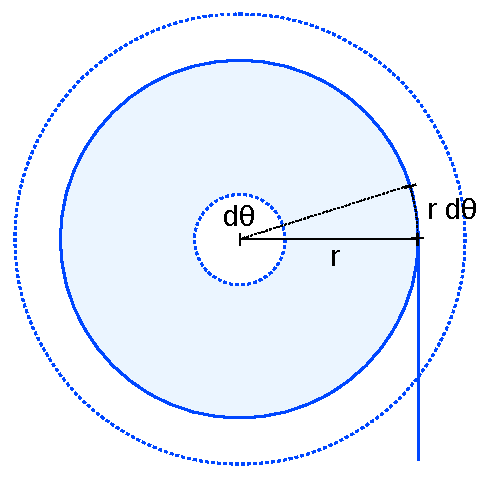
\includegraphics[height=2.5in]{figs/paper_roll.pdf}}
\caption{Diagram of a roll of toilet paper, showing change in paper length as a result of a small rotation, $d\theta$.}
\label{paper_roll}
\end{figure}

Figure~\ref{paper_roll} shows a diagram of the system: $r$ represents the radius of the roll at a point in time.  Initially, $r$ is the radius of the cardboard core, $R_{min}$.  When the roll is complete, $r$ is $R_{max}$.

I'll use $\theta$ to represent the total rotation of the roll in radians.  In the diagram, $d\theta$ represents a small increase in $\theta$, which corresponds to a distance along the circumference of the roll of $r~d\theta$.

\index{radian}

Finally, I'll use $y$ to represent the total length of paper that's been rolled.  Initially, $\theta=0$ and $y=0$.  For each small increase in $\theta$, there is a corresponding increase in $y$:
%
\[ dy = r~d\theta \]
%
If we divide both sides by a small increase in time, $dt$, we get a differential equation for $y$ as a function of time.
%
\[ \frac{dy}{dt} = r \frac{d\theta}{dt} \]
%
As we roll up the paper, $r$ increases, too.  Assuming that $r$ increases by a fixed amount per revolution, we can write
%
\[ dr = k~d\theta \]
%
Where $k$ is an unknown constant we'll have to figure out.  Again, we can divide both sides by $dt$ to get a differential equation in time:
%
\[ \frac{dr}{dt} = k \frac{d\theta}{dt} \]
%
Finally, let's assume that $\theta$ increases at a constant rate of \SI{10}{\radian\per\second} (about 95 revolutions per minute):
%
\[ \frac{d\theta}{dt} = 10  \]
%
This rate of change is called an {\bf angular velocity}.  Now we have a system of three differential equations we can use to simulate the system.

\index{angular velocity}
\index{differential equation}


\section{Implementation}
\label{papersim}

At this point we have a pretty standard process for writing simulations like this.  First, we'll get the units we need from Pint:
\index{Pint}

\begin{python}
radian = UNITS.radian
m = UNITS.meter
s = UNITS.second
\end{python}

And create a \py{Params} object with the parameters of the system:

\index{Params object}

\begin{python}
params = Params(Rmin = 0.02 * m,
                Rmax = 0.055 * m,
                L = 47 * m,
                omega = 10 * radian / s,
                t_end = 130 * s,
                dt = 1*s)
\end{python}

\py{Rmin} and \py{Rmax} are the initial and final values for the radius, \py{r}.  \py{L} is the total length of the paper. \py{t_end} is the length of the simulation in time, and \py{dt} is the time step for the ODE solver.

We use the \py{Params} object to make a \py{System} object:

\index{System object}
\index{\py{make_system}}

\begin{python}
def make_system(params):
    init = State(theta = 0 * radian,
                 y = 0 * m,
                 r = params.Rmin)
    
    k = estimate_k(params)

    return System(params, init=init, k=k)
\end{python}

The initial state contains three variables, \py{theta}, \py{y}, and \py{r}.

\py{estimate_k} computes the parameter, \py{k}, that relates \py{theta} and \py{r}.  Here's how it works:

\begin{python}
def estimate_k(params):
    Rmin, Rmax, L = params.Rmin, params.Rmax, params.L
    
    Ravg = (Rmax + Rmin) / 2
    Cavg = 2 * pi * Ravg
    revs = L / Cavg
    rads = 2 * pi * revs
    k = (Rmax - Rmin) / rads
    return k
\end{python}

\py{Ravg} is the average radius, half way between \py{Rmin} and \py{Rmax}, so \py{Cavg} is the circumference of the roll when \py{r} is \py{Ravg}.

\py{revs} is the total number of revolutions it would take to roll up length \py{L} if \py{r} were constant at \py{Ravg}.  And \py{rads} is just \py{revs} converted to radians.

Finally, \py{k} is the change in \py{r} for each radian of revolution.  For these parameters, \py{k} is about \py{2.8e-5} \si{\meter\per\radian}.

Now we can use the differential equations from Section~\ref{paper} to write a slope function:

\index{slope function}
\index{Function!slope}

\begin{python}
def slope_func(state, t, system):
    theta, y, r = state
    k, omega = system.k, system.omega
    
    dydt = r * omega
    drdt = k * omega
    
    return omega, dydt, drdt
\end{python}

\begin{figure}[t]
\centerline{\includegraphics[height=4.5in]{figs/chap24-fig01.pdf}}
\caption{Results from paper rolling simulation, showing rotation, length, and radius over time.}
\label{chap24-fig01}
\end{figure}

As usual, the slope function takes a \py{State} object, a time, and a \py{System} object.  The \py{State} object contains hypothetical values of \py{theta}, \py{y}, and \py{r} at time \py{t}.  The job of the slope function is to compute the time derivatives of these values.  The derivative of \py{theta} is angular velocity, which is often denoted \py{omega}.

\index{State object}

We'd like to stop the simulation when the length of paper on the roll is \py{L}.  We can do that with an event function that passes through 0 when \py{y} equals \py{L}:

\begin{python}
def event_func(state, t, system):
    theta, y, r = state
    return y - system.L
\end{python}

Now we can run the simulation like this:

\begin{python}
results, details = run_ode_solver(system, slope_func,
                                   events=event_func)
\end{python}


Figure~\ref{chap24-fig01} shows the results.  \py{theta} grows linearly over time, as we should expect.  As a result, \py{r} also grows linearly.  But since the derivative of \py{y} depends on \py{r}, and \py{r} is increasing, \py{y} grows with increasing slope.

Because this system is so simple, it is almost silly to simulate it.  As we'll see in the next section, it is easy enough to solve the differential equations analytically.  But it is often useful to start with a simple simulation as a way of exploring and checking assumptions.

In order to get the simulation working, we have to get the units right, which can help catch conceptual errors early.  And by plugging in realistic parameters, we can detect errors that cause unrealistic results.  For example, in this system we can check:

\begin{itemize}

\item The total time for the simulation is about 2 minutes, which seems plausible for the time it would take to roll \SI{47}{\meter} of paper.

\item The final value of \py{theta} is about \SI{1250}{\radian}, which corresponds to about 200 revolutions, which also seems plausible.

\item The initial and final values for \py{r} are consistent with \py{Rmin} and \py{Rmax}, as we intended when we chose \py{k}.

\end{itemize}

But now that we have a working simulation, it is also useful to do some analysis.


\section{Analysis}
\label{paper_analysis}

The differential equations in Section~\ref{paper} are simple enough that we can just solve them.  Since angular velocity is constant:
%
\[ \frac{d\theta}{dt} = \omega  \]
%
We can find $\theta$ as a function of time by integrating both sides:
%
\[ \theta(t) = \omega t + C_1 \]
%
With the initial condition $\theta(0)=0$,  we find $C_1=0$.  Similarly,
%
\begin{equation}
\frac{dr}{dt} = k \omega                    \label{eqn1}
\end{equation}
%
So
%
\[ r(t) = k \omega t + C_2 \]
%
With the initial condition $r(0)=R_{min}$,  we find $C_2=R_{min}$.  Then we can plug the solution for $r$ into the equation for $y$:
%
\begin{align}
\frac{dy}{dt} & = r \omega                    \label{eqn2}   \\
              & = \left[ k \omega t + R_{min} \right] \omega \nonumber
\end{align}
%
%
Integrating both sides yields:
%
\[ y(t) = \left[ k \omega t^2 / 2 + R_{min} t \right] \omega + C_3\]
%
So $y$ is a parabola, as you might have guessed.  With initial condition $y(0)=0$, we find $C_3=0$.

\index{analysis}
\index{integration}

We can also use these equations to find the relationship between $y$ and $r$, independent of time, which we can use to compute $k$.  Using a move we saw in Section~\ref{contact}, I'll divide Equations~\ref{eqn1} and \ref{eqn2}, yielding
%
\[ \frac{dr}{dy} = \frac{k}{r}\]
%
Separating variables yields
%
\[ r~dr = k~dy\]
%
Integrating both sides yields
%
\[ r^2 / 2 = k y + C \]
%
When $y=0$, $r=R_{min}$, so
%
\[ C = \frac{1}{2} R_{min}^2 \]
%
Solving for $y$, we have
%
\begin{equation}
y = \frac{1}{2k} (r^2 - R_{min}^2)                 \label{eqn3}
\end{equation}
%
When $y=L$, $r=R_{max}$; substituting in those values yields
%
\[ L = \frac{1}{2k} (R_{max}^2 - R_{min}^2) \]
%
Solving for $k$ yields
%
\begin{equation}
k =  \frac{1}{2L} (R_{max}^2 - R_{min}^2)           \label{eqn4}
\end{equation}
%
Plugging in the values of the parameters yields \py{2.8e-5} \si{\meter\per\radian}, the same as the ``estimate" we computed in Section~\ref{papersim}.  In this case the estimate turns out to be exact.

Before you go on, you might want to read the notebook for this chapter, \py{chap24.ipynb}, and work on the exercises.  For instructions on downloading and running the code, see Section~\ref{code}.


\chapter{Torque}
\label{chap25}

In the previous chapter we modeled a scenario with constant angular velocity.  In this chapter we make it more complex; we'll model a teapot, on a turntable, revolving with constant angular acceleration and deceleration.

\section{Angular acceleration}

\index{angular acceleration}
\index{torque}

Just as linear acceleration is the derivative of velocity, {\bf angular acceleration} is the derivative of angular velocity.  And just as linear acceleration is caused by force, angular acceleration is caused by the rotational version of force, {\bf torque}.  If you are not familiar with torque, you can read about it at \url{http://modsimpy.com/torque}.

In general, torque is a vector quantity, defined as the {\bf cross product} of $\vec{r}$ and $\vec{F}$, where $\vec{r}$ is the {\bf lever arm}, a vector from the point of rotation to the point where the force is applied, and $\vec{F}$ is the vector that represents the magnitude and direction of the force.

\index{vector}
\index{lever arm}
\index{cross product}

However, for the problems in this chapter, we only need the {\em magnitude} of torque; we don't care about the direction.  In that case, we can compute
%
\[ \tau = r F \sin \theta \]
%
where $\tau$ is torque, $r$ is the length of the lever arm, $F$ is the magnitude of force, and $\theta$ is the angle between $\vec{r}$ and $\vec{F}$.  

\index{magnitude}

Since torque is the product of a length and a force, it is expressed in newton meters (\si{\newton\meter}).


\section{Moment of inertia}

In the same way that linear acceleration is related to force by Newton's second law of motion, $F=ma$, angular acceleration is related to torque by another form of Newton's law:
%
\[ \tau = I \alpha \]
%
Where $\alpha$ is angular acceleration and $I$ is {\bf moment of inertia}.  Just as mass is what makes it hard to accelerate an object\footnote{That might sound like a dumb way to describe mass, but its actually one of the fundamental definitions.}, moment of inertia is what makes it hard to spin an object.

\index{mass}
\index{moment of inertia}

In the most general case, a 3-D object rotating around an arbitrary axis, moment of inertia is a tensor, which is a function that takes a vector as a parameter and returns a vector as a result.

\index{tensor}

Fortunately, in a system where all rotation and torque happens around a single axis, we don't have to deal with the most general case.  We can treat moment of inertia as a scalar quantity.

\index{scalar}

For a small object with mass $m$, rotating around a point at distance $r$, the moment of inertia is $I = m r^2$.  For more complex objects, we can compute $I$ by dividing the object into small masses, computing moments of inertia for each mass, and adding them up.

However, for most simple shapes, people have already done the calculations; you can just look up the answers.  For example, see \url{http://modsimpy.com/moment}.


\section{Teapots and turntables}

Tables in Chinese restaurants often have a rotating tray or turntable
that makes it easy for customers to share dishes. These turntables are
supported by low-friction bearings that allow them to turn easily and
glide. However, they can be heavy, especially when they are loaded with
food, so they have a high moment of inertia.

\index{teapot}
\index{turntable}

Suppose I am sitting at a table with a pot of tea on the turntable
directly in front of me, and the person sitting directly opposite asks
me to pass the tea. I push on the edge of the turntable with \SI{1}{\newton} of force until it has turned \SI{0.5}{\radian}, then let go. The turntable glides until it comes to a stop \SI{1.5}{\radian} from the starting position. How much force should I apply for a second push so the teapot glides to a
stop directly opposite me?

\index{force}
\index{Newton}
\index{friction}

We'll answer this question in these steps:

\begin{enumerate}

\item
  I'll use the results from the first push to estimate the coefficient
  of friction for the turntable.

\item
  As an exercise, you'll use that coefficient of friction to estimate the force needed to rotate the turntable through the remaining angle.

\end{enumerate}

Our simulation will use the following parameters:

\begin{enumerate}

\item
  The radius of the turntable is \SI{0.5}{\meter}, and its weight is \SI{7}{\kg}.
  
\item
  The teapot weights \SI{0.3}{\kg}, and it sits \SI{0.4}{\meter} from the center of the turntable.

\end{enumerate}

\begin{figure}
\centerline{\includegraphics[height=2.5in]{figs/teapot.pdf}}
\caption{Diagram of a turntable with a teapot.}
\label{teapot}
\end{figure}

Figure~\ref{teapot} shows the scenario, where $F$ is the force I apply to the turntable at the perimeter, perpendicular to the moment arm, $r$, and $\tau$ is the resulting torque. The blue circle near the bottom is the teapot.

Here's a \py{Params} object with the parameters of the scenario:

\begin{python}
params = Params(radius_disk=0.5*m,
                mass_disk=7*kg,
                radius_pot=0.4*m,
                mass_pot=0.3*kg,
                force=1*N,
                torque_friction=0.2*N*m,
                theta_end=0.5*radian,
                t_end=20*s)
\end{python}

\index{Params object}

\py{make_system} creates the initial state, \py{init}, and
computes the total moment of inertia for the turntable and the teapot.

\begin{python}
def make_system(params):
    mass_disk, mass_pot = params.mass_disk, params.mass_pot
    radius_disk, radius_pot = params.radius_disk, params.radius_pot
    
    init = State(theta=0*radian, omega=0*radian/s)
    
    I_disk = mass_disk * radius_disk**2 / 2
    I_pot = mass_pot * radius_pot**2
    
    return System(params, init=init, I=I_disk+I_pot)
\end{python}

%\index{make_system}

In the initial state,
\py{theta} represents the angle of the table in \si{\radian}; \py{omega} represents the angular velocity in \si{\radian\per\second}.

\py{I_disk} is the moment of inertia of the turntable, which is based on the moment of inertia for a horizontal disk revolving around a vertical axis through its center:
%
\[ I_{disk} = m r^2 / 2 \]
%
\py{I_pot} is the moment of inertia of the teapot, which I treat as a point mass with:
%
\[ I_{point} = m r^2 \]
%
In SI units, moment of inertia is expressed in \si{\kilogram\meter\squared}.  

Now we can make a \py{System} object:

\begin{python}
system1 = make_system(params)
\end{python}

\index{System object}

Here's a slope that takes the current state, which contains angle and angular velocity, and returns the derivatives, angular velocity and angular acceleration:

\begin{python}
def slope_func(state, t, system):
    theta, omega = state
    radius_disk, force = system.radius_disk, system.force
    torque_friction, I = system.torque_friction, system.I
    
    torque = radius_disk * force - torque_friction
    alpha = torque / I
    
    return omega, alpha 
\end{python}

\index{slope function}

In this scenario, the force I apply to the turntable is always perpendicular to the lever arm, so $\sin \theta = 1$ and the torque due to force is $\tau = r F$.

\py{torque_friction} represents the torque due to friction.  Because the turntable is rotating in the direction of positive \py{theta}, friction acts in the direction of negative \py{theta}.

\index{friction}

Now we are ready to run the simulation, but first there's a problem we have to address.

When I stop pushing on the turntable, the angular acceleration changes
abruptly. We could implement the slope function with an \py{if}
statement that checks the value of \py{theta} and sets
\py{force} accordingly. And for a coarse model like this one, that
might be fine. But we will get more accurate results if we simulate the
system in two phases:

\begin{enumerate}
\item
  During the first phase, force is constant, and we run until
  \py{theta} is 0.5 radians.
\item
  During the second phase, force is 0, and we run until \py{omega}
  is 0.
\end{enumerate}

Then we can combine the results of the two phases into a single
\py{TimeFrame}.

\index{two-phase simulation}

Here's the event function I'll use for Phase 1; it stops the simulation when \py{theta} reaches \py{theta_end}, which is when I stop pushing:

\begin{python}
def event_func1(state, t, system):
    theta, omega = state
    return theta - system.theta_end 
\end{python}

Now we can run the first phase.

\begin{python}
results1, details1 = run_ode_solver(system1, slope_func,
                                      events=event_func1)
\end{python}

%\index{run_ode_solver}

\begin{figure}
\centerline{\includegraphics[height=4.0in]{figs/chap25-fig01.pdf}}
\caption{Angle and angular velocity of a turntable with applied force and friction.}
\label{chap25-fig01}
\end{figure}

Before we run the second phase, we have to extract the final time and
state of the first phase.

\begin{python}
t_0 = get_last_label(results1) * s
init2 = results1.last_row()
\end{python}

Now we can make a \py{System} object for Phase 2, with the initial state from Phase 1, and with \py{force=0}.

%\index{get_last_label}
%\index{get_last_value}

\begin{python}
system2 = System(system1, t_0=t_0, init=init2, force=0*N)
\end{python}

For the second phase, we need an event function that stops when the turntable stops; that is, when angular velocity is 0.

\begin{python}
def event_func2(state, t, system):
    theta, omega = state
    return omega
\end{python}

Now we can run the second phase.

\begin{python}
results2, details2 = run_ode_solver(system2, slope_func,
                                      events=event_func2)
\end{python}

Pandas provides \py{combine_first}, which combines
\py{results1} and \py{results2}.

\index{Pandas}

\begin{python}
results = results1.combine_first(results2)
\end{python}

Figure~\ref{chap25-fig01} shows the results.  Angular velocity, \py{omega}, increases linearly while I am pushing, and decreases linearly after I let go.  The angle, \py{theta}, is the integral of angular velocity, so it forms a parabola during each phase.

In the next section, we'll use this simulation to estimate the torque due to friction.


\section{Estimating friction}

Let's take the code from the previous section and wrap it in a function.

\index{function}

\begin{python}
def run_two_phases(force, torque_friction, params):
    # put the parameters into the Params object
    params = Params(params, force=force, 
                    torque_friction=torque_friction)

    # run phase 1
    system1 = make_system(params)
    results1, details1 = run_ode_solver(system1, slope_func, 
                                          events=event_func1)

    # get the final state from phase 1
    t_0 = results1.last_label() * s
    init2 = results1.last_row()
    
    # run phase 2
    system2 = System(system1, t_0=t_0, init=init2, force=0*N)
    results2, details2 = run_ode_solver(system2, slope_func, 
                                          events=event_func2)
    
    # combine and return the results
    results = results1.combine_first(results2)
    return TimeFrame(results)
\end{python}

We can use \py{run_two_phases} to write an error function we can use, with \py{root_bisect}, to find the torque due to friction that yields the observed results from the first push, a total rotation of \SI{1.5}{\radian}.

\index{\py{root_bisect}}
\index{error function}

\begin{python}
def error_func1(torque_friction, params):
    force = 1 * N
    results = run_two_phases(force, torque_friction, params)
    theta_final = results.last_row().theta
    print(torque_friction, theta_final)
    return theta_final - 1.5 * radian
\end{python}

Now we can use \py{root_bisect} to estimate torque due to friction.

\index{torque}
\index{friction}
\index{\py{root_bisect}}

\begin{python}
res = root_bisect(error_func1, [0.5, 2], params)
force = res.root
\end{python}

The result is \SI{0.166}{\newton\meter}, a little less than the initial guess.

Now that we know the torque due to friction, we can compute the force needed to rotate the turntable through the remaining angle, that is, from \SI{1.5}{\radian} to \SI{3.14}{\radian}.

In the notebook for this chapter, \py{chap25.ipynb}, you will have a chance to finish off the exercise.  For instructions on downloading and running the code, see Section~\ref{code}.


\chapter{Case studies}
\label{chap26}

\section{Computational tools}

In Chapter~\ref{chap20} we rewrote a second order differential equation as a system of first order equations, and solved them using a slope function like this:

\begin{python}
def slope_func(state, t, system):
    y, v = state
    g = system.g    

    dydt = v
    dvdt = -g
    
    return dydt, dvdt
\end{python}

We used the \py{crossings} function to search for zero-crossings in the simulation results.

Then we used an event function like this:

\begin{python}
def event_func(state, t, system):
    y, v = state
    return y
\end{python}

To stop the simulation when an event occurs.  Notice that the event function takes the same parameters as the slope function.

In Chapter~\ref{chap21} we developed a model of air resistance and used a  \py{Params} object, which is a collection of parameters:

\begin{python}
params = Params(height = 381 * m,
                v_init = 0 * m / s,
                g = 9.8 * m/s**2,
                mass = 2.5e-3 * kg,
                diameter = 19e-3 * m,
                rho = 1.2 * kg/m**3,
                v_term = 18 * m / s)
\end{python}

And we saw a new way to create a \py{System} object, copying the variables from a \py{Params} object and adding or changing variables:

\begin{python}
    return System(params, area=area, C_d=C_d, 
                  init=init, t_end=t_end)
\end{python}

We also used the \py{gradient} function to estimate acceleration, given velocity:

\begin{python}
a = gradient(results.v)
\end{python}

Chapter~\ref{chap22} introduces \py{Vector} objects, which can represent vector quantities, like position, velocity, force, and acceleration, in 2 or 3 dimensions.

\begin{python}
A = Vector(3, 4) * m
\end{python}

It also introduces trajectory plots, which show the path of an object in two dimensions:

\begin{python}
x = results.R.extract('x')
y = results.R.extract('y')

plot(x, y, label='trajectory')
\end{python}

In Chapter~\ref{chap23} we define a range function that computes the distance a baseball flies as a function of launch angle:

\begin{python}
def range_func(angle, params):  
    params = Params(params, angle=angle)
    system = make_system(params)
    results, details = run_ode_solver(system, slope_func,
                                       events=event_func)
    x_dist = get_last_value(results.R).x
    return x_dist
\end{python}

Then we use \py{maximize} to find the launch angle that maximizes range:

\begin{python}
bounds = [0, 90] * degree
res = maximize(range_func, bounds, params)
\end{python}

With that, your toolkit is complete.  Chapter~\ref{chap24} and Chapter~\ref{chap25} introduce the physics of rotation, but no new computational tools.


\section{Bungee jumping}
\label{bungee}

Suppose you want to set the world record for the highest ``bungee dunk", which is a stunt in which a bungee jumper dunks a cookie in a cup of tea at the lowest point of a jump.  An example is shown in this video: \url{http://modsimpy.com/dunk}.

Since the record is \SI{70}{\meter}, let's design a jump for \SI{80}{\meter}.  We'll start with the following modeling assumptions:

\begin{itemize}

\item  Initially the bungee cord hangs from a crane with the attachment point \SI{80}{\meter} above a cup of tea.

\item Until the cord is fully extended, it applies no force to the jumper.  It turns out this might not be a good assumption; we will revisit it.

\item After the cord is fully extended, it obeys Hooke's Law; that is, it applies a force to the jumper proportional to the extension of the cord beyond its resting length.  See \url{http://modsimpy.com/hooke}. 

\item The mass of the jumper is \SI{75}{\kilogram}.

\item The jumper is subject to drag force so that their terminal velocity is \SI{60}{\meter \per \second}.

\end{itemize}

Our objective is to choose the length of the cord, \py{L}, and its spring constant, \py{k}, so that the jumper falls all the way to the tea cup, but no farther!

In the repository for this book, you will find a notebook, \py{bungee.ipynb}, which contains starter code and exercises for this case study.


\section{Bungee dunk revisited}

In the previous case study, we assume that the cord applies no force to the jumper until it is stretched.
It is tempting to say that the cord has no effect because it falls along with the jumper, but that intuition is incorrect.  As the cord falls, it transfers energy to the jumper.

\index{bungee jump}
\index{bungee cord}

At \url{http://modsimpy.com/bungee} you'll find a paper\footnote{Heck, Uylings, and Kędzierska, ``Understanding the physics of bungee jumping", Physics Education, Volume 45, Number 1, 2010.} that explains this phenomenon and derives the acceleration of the jumper, $a$, as a function of position, $y$, and velocity, $v$:
%
\[ a = g + \frac{\mu v^2/2}{\mu(L+y) + 2L} \] 
%
where $g$ is acceleration due to gravity, $L$ is the length of the cord, and $\mu$ is the ratio of the mass of the cord, $m$, and the mass of the jumper, $M$.

If you don't believe that their model is correct, this video might convince you: \url{http://modsimpy.com/drop}.

In the repository for this book, you will find a notebook, \py{bungee2.ipynb}, which contains starter code and exercises for this case study.
How does the behavior of the system change as we vary the mass of the cord?
When the mass of the cord equals the mass of the jumper, what is the net effect on the lowest point in the jump?



\section{Spider-Man}

In this case study we'll develop a model of Spider-Man swinging from a
springy cable of webbing attached to the top of the Empire State
Building.  Initially, Spider-Man is at the top of a nearby building, as
shown in Figure~\ref{spiderman}.

\index{Spider-man}
\index{Empire State Building}

\begin{figure}
\centerline{\includegraphics[height=2.8in]{figs/spiderman.pdf}}
\caption{Diagram of the initial state for the Spider-Man case study.}
\label{spiderman}
\end{figure}

The origin, \texttt{O}, is at the base of the Empire State Building. The
vector \py{H} represents the position where the webbing is attached
to the building, relative to \py{O}. The vector \py{P} is the
position of Spider-Man relative to \py{O}. And \py{L} is the
vector from the attachment point to Spider-Man.

\index{vector}

By following the arrows from \py{O}, along \py{H}, and along
\py{L}, we can see that

\begin{code}
H + L = P
\end{code}

So we can compute \py{L} like this:

\begin{code}
L = P - H
\end{code}

The goals of this case study are:

\begin{enumerate}

\item
  Implement a model of this scenario to predict Spider-Man's trajectory.
\index{trajectory}

\item
  Choose the right time for Spider-Man to let go of the webbing in order
  to maximize the distance he travels before landing.
\index{range}

\item
  Choose the best angle for Spider-Man to jump off the building, and let
  go of the webbing, to maximize range.
\index{optimization}  
  
\end{enumerate}

We'll use the following parameters:
\index{parameter}

\begin{enumerate}

\item According to the Spider-Man Wiki\footnote{\url{http://modsimpy.com/spider}}, Spider-Man weighs \SI{76}{\kg}.

\item
  Let's assume his terminal velocity is \SI{60}{\meter\per\second}.
\index{terminal velocity}

\item
  The length of the web is \SI{100}{\meter}.

\item
  The initial angle of the web is \SI{45}{\degree} to the left of straight
  down.

\item
  The spring constant of the web is \SI{40}{\newton\per\meter} when the cord is stretched, and 0 when it's compressed.

\end{enumerate}

In the repository for this book, you will find a notebook, \py{spiderman.ipynb}, which contains starter code.   Read through the notebook and run the code.  It uses \py{minimize}, which is a SciPy function that can search for an optimal set of parameters (as contrasted with \py{minimize_scalar}, which can only search along a single axis).


\section{Kittens}

Let's simulate a kitten unrolling toilet paper.  As reference material, see this video: \url{http://modsimpy.com/kitten}.

\index{kitten}

The interactions of the kitten and the paper roll are complex.  To keep things simple, let's assume that the kitten pulls down on the free end of the roll with constant force.  Also, we will neglect the friction between the roll and the axle.  

\begin{figure}
\centerline{\includegraphics[height=2.5in]{figs/kitten.pdf}}
\caption{Diagram of a roll of toilet paper, showing a force, lever arm, and the resulting torque.}
\label{kitten}
\end{figure}

Figure~\ref{kitten} shows the paper roll with $r$, $F$, and $\tau$.  As a vector quantity, the direction of $\tau$ is into the page, but we only care about its magnitude for now.

Here's the \py{Params} object with the parameters we'll need:

\index{Params object}

\begin{python}
params = Params(Rmin = 0.02 * m,
                Rmax = 0.055 * m,
                Mcore = 15e-3 * kg,
                Mroll = 215e-3 * kg,
                L = 47 * m,
                tension = 2e-4 * N,
                t_end = 180 * s)
\end{python}

As before, \py{Rmin} is the minimum radius and \py{Rmax} is the maximum.  \py{L} is the length of the paper.  \py{Mcore} is the mass of the cardboard tube at the center of the roll; \py{Mroll} is the mass of the paper.  \py{tension} is the force applied by the kitten, in \si{\newton}.  I chose a value that yields plausible results.

At \url{http://modsimpy.com/moment} you can find moments of inertia for simple geometric shapes.  I'll model the cardboard tube at the center of the roll as a ``thin cylindrical shell", and the paper roll as a ``thick-walled cylindrical tube with open ends".

\index{cylinder}

The moment of inertia for a thin shell is just $m r^2$, where $m$ is the mass and $r$ is the radius of the shell.

For a thick-walled tube the moment of inertia is
%
\[ I = \frac{\pi \rho h}{2} (r_2^4 - r_1^4) \]
%
where $\rho$ is the density of the material, $h$ is the height of the tube, $r_2$ is the outer diameter, and $r_1$ is the inner diameter.

Since the outer diameter changes as the kitten unrolls the paper, we have to compute the moment of inertia, at each point in time, as a function of the current radius, \py{r}.  Here's the function that does it:

\index{unpack}

\begin{python}
def moment_of_inertia(r, system):
    Mcore, Rmin = system.Mcore, system.Rmin
    rho_h = system.rho_h
    
    Icore = Mcore * Rmin**2   
    Iroll = pi * rho_h / 2 * (r**4 - Rmin**4)
    return Icore + Iroll
\end{python}

\py{rho_h} is the product of density and height, $\rho h$, which is the mass per area.  \py{rho_h} is computed in \py{make_system}:

\index{density}
\index{\py{make_system}}

\begin{python}
def make_system(params):
    L, Rmax, Rmin = params.L, params.Rmax, params.Rmin
    Mroll = params.Mroll
    
    init = State(theta = 0 * radian,
                 omega = 0 * radian/s,
                 y = L)
    
    area = pi * (Rmax**2 - Rmin**2)
    rho_h = Mroll / area
    k = (Rmax**2 - Rmin**2) / 2 / L / radian    
    
    return System(params, init=init, area=area, 
                  rho_h=rho_h, k=k)
\end{python}

\py{make_system} also computes \py{k} using Equation~\ref{eqn4}.

In the repository for this book, you will find a notebook, \py{kitten.ipynb}, which contains starter code for this case study.   Use it to implement this model and check whether the results seem plausible.


\section{Simulating a yo-yo}

Suppose you are holding a yo-yo with a length of string wound around its axle, and you drop it while holding the end of the string stationary.  As gravity accelerates the yo-yo downward, tension in the string exerts a force upward.  Since this force acts on a point offset from the center of mass, it exerts a torque that causes the yo-yo to spin.

\index{yo-yo}
\index{torque}
\index{lever arm}

\begin{figure}
\centerline{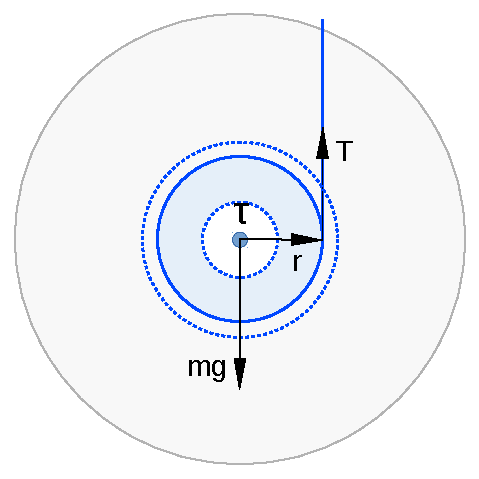
\includegraphics[height=2.5in]{figs/yoyo.pdf}}
\caption{Diagram of a yo-yo showing forces due to gravity and tension in the string, the lever arm of tension, and the resulting torque.}
\label{yoyo}
\end{figure}

Figure~\ref{yoyo} is a diagram of the forces on the yo-yo and the resulting torque.  The outer shaded area shows the body of the yo-yo.  The inner shaded area shows the rolled up string, the radius of which changes as the yo-yo unrolls.

\index{system of equations}

In this model, we can't figure out the linear and angular acceleration independently; we have to solve a system of equations:
%
\begin{align*}
\sum F &= m a \\
\sum \tau &= I \alpha
\end{align*}
%
where the summations indicate that we are adding up forces and torques.

As in the previous examples, linear and angular velocity are related because of the way the string unrolls:
%
\[ \frac{dy}{dt} = -r \frac{d \theta}{dt} \]
%
In this example, the linear and angular accelerations have opposite sign.  As the yo-yo rotates counter-clockwise, $\theta$ increases and $y$, which is the length of the rolled part of the string, decreases.

Taking the derivative of both sides yields a similar relationship between linear and angular acceleration:
%
\[ \frac{d^2 y}{dt^2} = -r \frac{d^2 \theta}{dt^2} \]
%
Which we can write more concisely:
%
\[ a = -r \alpha \]
%
This relationship is not a general law of nature; it is specific to scenarios like this where one object rolls along another without stretching or slipping.

\index{rolling}

Because of the way we've set up the problem, $y$ actually has two meanings: it represents the length of the rolled string and the height of the yo-yo, which decreases as the yo-yo falls.  Similarly, $a$ represents acceleration in the length of the rolled string and the height of the yo-yo.

We can compute the acceleration of the yo-yo by adding up the linear forces:
%
\[ \sum F = T - mg = ma \]
%
Where $T$ is positive because the tension force points up, and $mg$ is negative because gravity points down.

Because gravity acts on the center of mass, it creates no torque, so the only torque is due to tension:
%
\[ \sum \tau = T r = I \alpha \]
%
Positive (upward) tension yields positive (counter-clockwise) angular acceleration.

\index{SymPy}

Now we have three equations in three unknowns, $T$, $a$, and $\alpha$, with $I$, $m$, $g$, and $r$ as known quantities.  It is simple enough to solve these equations by hand, but we can also get SymPy to do it for us:

\begin{python}
T, a, alpha, I, m, g, r = symbols('T a alpha I m g r')
eq1 = Eq(a, -r * alpha)
eq2 = Eq(T - m*g, m * a)
eq3 = Eq(T * r, I * alpha)
soln = solve([eq1, eq2, eq3], [T, a, alpha])
\end{python}

The results are
%
\begin{align*}
T      &= m g I / I^*   \\
a      &= -m g r^2 / I^* \\
\alpha &= m g r / I^*    \\
\end{align*}
%
where $I^*$ is the augmented moment of inertia, $I + m r^2$.
To simulate the system, we don't really need $T$; we can plug $a$ and $\alpha$ directly into the slope function.

In the repository for this book, you will find a notebook, \py{yoyo.ipynb}, which contains the derivation of these equations and starter code for this case study.   Use it to implement and test this model.


%\section{Rigid pendulum}

%\section{LRC circuit}

% Pendulum:

% Springy pendulum

% Stiff problem as k increases

% Add drag

% Rigid pendulum: solve those constraints

% Generalized coordinates


\backmatter
\printindex

%\afterpage{\blankpage}


\end{document}

\end{itemize}


\section{Under the hood}

Throughout this book, we'll use functions defined in the ModSim library.  You don't have to know how they work, but you might be curious.  So at the end of some chapters I'll provide additional information.  If you are an experienced programmer, you might be interested by the design decisions I made.  If you are a beginner, and you feel like you have your hands full already, feel free to skip these sections.

\index{modsim}

Most of the functions in \py{modsim} are based on other Python libraries; the libraries we have used so far include:

\begin{itemize}

\item {\bf Pint}, which provides units like meters and seconds, as we saw in Section~\ref{penny}.

\item {\bf NumPy}, which provides mathematical operations like \py{sqrt}, which we saw in Section~\ref{computation}.

\item {\bf Pandas}, which provides the \py{Series} object, which is the basis of the \py{State} object in Section~\ref{modeling}.

\item {\bf Pyplot}, which provides plotting functions, as we saw in Section~\ref{plotting}.

\end{itemize}

You could use these libraries directly, and when you have more experience, you probably will.  But the functions in \py{modsim} are meant to be easier to use; they provide some additional capabilities, including error checking; and by hiding details you don't need to know about, they let you focus on more important things.

However, there are drawbacks.  One is that it can be hard to understand the error messages.  I'll have more to say about this in later chapters, but for now I have a suggestion.  When you are getting started, you should practice making errors.

\index{debugging}

For each new function you learn, you should deliberately make as many mistakes as possible so you can see what happens.  When you see what the errors messages are, you will understand what they mean.  And that should help later, when you make errors accidentally.


